%%%%%%%%%%%%%%%%%%%%%%%%%%%%%%%%%%%%%%%%%%%%%%%%%%%%%%%%%%%%%%%
%% OXFORD THESIS TEMPLATE

% Use this template to produce a standard thesis that meets the Oxford University requirements for DPhil submission
%
% Originally by Keith A. Gillow (gillow@maths.ox.ac.uk), 1997
% Modified by Sam Evans (sam@samuelevansresearch.org), 2007
% Modified by John McManigle (john@oxfordechoes.com), 2015
% Modified by Ulrik Lyngs (ulrik.lyngs@cs.ox.ac.uk), 2018-, for use with R Markdown
%
% Ulrik Lyngs, 25 Nov 2018: Following John McManigle, broad permissions are granted to use, modify, and distribute this software
% as specified in the MIT License included in this distribution's LICENSE file.
%
% John commented this file extensively, so read through to see how to use the various options.  Remember that in LaTeX,
% any line starting with a % is NOT executed.  Several places below, you have a choice of which line to use
% out of multiple options (eg draft vs final, for PDF vs for binding, etc.)  When you pick one, add a % to the beginning of
% the lines you don't want.


%%%%% PAGE LAYOUT
% The most common choices should be below.  You can also do other things, like replacing "a4paper" with "letterpaper", etc.

% This one formats for two-sided binding (ie left and right pages have mirror margins; blank pages inserted where needed):
%\documentclass[a4paper,twoside]{templates/ociamthesis}
% This one formats for one-sided binding (ie left margin > right margin; no extra blank pages):
%\documentclass[a4paper]{ociamthesis}
% This one formats for PDF output (ie equal margins, no extra blank pages):
%\documentclass[a4paper,nobind]{templates/ociamthesis}

% As you can see from the uncommented line below, oxforddown template uses the a4paper size, 
% and passes in the binding option from the YAML header in index.Rmd:
\documentclass[a4paper, nobind]{templates/ociamthesis}


%%%%% ADDING LATEX PACKAGES
% add hyperref package with options from YAML %
\usepackage[pdfpagelabels]{hyperref}
% change the default coloring of links to something sensible
\usepackage{xcolor}

\definecolor{mylinkcolor}{RGB}{0,0,139}
\definecolor{myurlcolor}{RGB}{0,0,139}
\definecolor{mycitecolor}{RGB}{0,33,71}

\hypersetup{
  hidelinks,
  colorlinks,
  linktocpage=true,
  linkcolor=mylinkcolor,
  urlcolor=myurlcolor,
  citecolor=mycitecolor
}



% add float package to allow manual control of figure positioning %
\usepackage{float}

% enable strikethrough
\usepackage[normalem]{ulem}

% use soul package for correction highlighting
\usepackage{color, soul}
\definecolor{correctioncolor}{HTML}{CCCCFF}
\sethlcolor{correctioncolor}
\newcommand{\ctext}[3][RGB]{%
  \begingroup
  \definecolor{hlcolor}{#1}{#2}\sethlcolor{hlcolor}%
  \hl{#3}%
  \endgroup
}
\soulregister\ref7
\soulregister\cite7
\soulregister\autocite7
\soulregister\textcite7
\soulregister\pageref7

%%%%% FIXING / ADDING THINGS THAT'S SPECIAL TO R MARKDOWN'S USE OF LATEX TEMPLATES
% pandoc puts lists in 'tightlist' command when no space between bullet points in Rmd file,
% so we add this command to the template
\providecommand{\tightlist}{%
  \setlength{\itemsep}{0pt}\setlength{\parskip}{0pt}}
 
% UL 1 Dec 2018, fix to include code in shaded environments

% User-included things with header_includes or in_header will appear here
% kableExtra packages will appear here if you use library(kableExtra)
\usepackage{booktabs}
\usepackage{longtable}
\usepackage{array}
\usepackage{multirow}
\usepackage{wrapfig}
\usepackage{float}
\usepackage{colortbl}
\usepackage{pdflscape}
\usepackage{tabu}
\usepackage{threeparttable}
\usepackage{threeparttablex}
\usepackage[normalem]{ulem}
\usepackage{makecell}
\usepackage{xcolor}


%UL set section header spacing
\usepackage{titlesec}
% 
\titlespacing\subsubsection{0pt}{24pt plus 4pt minus 2pt}{0pt plus 2pt minus 2pt}


%UL set whitespace around verbatim environments
\usepackage{etoolbox}
\makeatletter
\preto{\@verbatim}{\topsep=0pt \partopsep=0pt }
\makeatother



%%%%%%% PAGE HEADERS AND FOOTERS %%%%%%%%%
\usepackage{fancyhdr}
\setlength{\headheight}{15pt}
\fancyhf{} % clear the header and footers
\pagestyle{fancy}
\renewcommand{\chaptermark}[1]{\markboth{\thechapter. #1}{\thechapter. #1}}
\renewcommand{\sectionmark}[1]{\markright{\thesection. #1}} 
\renewcommand{\headrulewidth}{0pt}

\fancyhead[LO]{\emph{\leftmark}} 
\fancyhead[RE]{\emph{\rightmark}} 

% UL page number position 
\fancyfoot[C]{\emph{\thepage}} %regular pages
\fancypagestyle{plain}{\fancyhf{}\fancyfoot[C]{\emph{\thepage}}} %chapter pages

% JEM fix header on cleared pages for openright
\def\cleardoublepage{\clearpage\if@twoside \ifodd\c@page\else
   \hbox{}
   \fancyfoot[C]{}
   \newpage
   \if@twocolumn\hbox{}\newpage
   \fi
   \fancyhead[LO]{\emph{\leftmark}} 
   \fancyhead[RE]{\emph{\rightmark}} 
   \fi\fi}


%%%%% SELECT YOUR DRAFT OPTIONS
% This adds a "DRAFT" footer to every normal page.  (The first page of each chapter is not a "normal" page.)

% IP feb 2021: option to include line numbers in PDF

% for line wrapping in code blocks
\usepackage{fvextra}
\DefineVerbatimEnvironment{Highlighting}{Verbatim}{breaklines,commandchars=\\\{\}}

% This highlights (in blue) corrections marked with (for words) \mccorrect{blah} or (for whole
% paragraphs) \begin{mccorrection} . . . \end{mccorrection}.  This can be useful for sending a PDF of
% your corrected thesis to your examiners for review.  Turn it off, and the blue disappears.
\correctionstrue


%%%%% BIBLIOGRAPHY SETUP
% Note that your bibliography will require some tweaking depending on your department, preferred format, etc.
% If you've not used LaTeX before, I recommend reading a little about biblatex/biber and getting started with it.
% If you're already a LaTeX pro and are used to natbib or something, modify as necessary.
% Either way, you'll have to choose and configure an appropriate bibliography format...


\usepackage[style=authoryear, sorting=nyt, backend=biber, maxcitenames=2, useprefix, doi=true, isbn=false, uniquename=false]{biblatex}
\newcommand*{\bibtitle}{Works Cited}

\addbibresource{bibliography/references.bib}
\addbibresource{bibliography/additional-references.bib}


% This makes the bibliography left-aligned (not 'justified') and slightly smaller font.
\renewcommand*{\bibfont}{\raggedright\small}


% Uncomment this if you want equation numbers per section (2.3.12), instead of per chapter (2.18):
%\numberwithin{equation}{subsection}


%%%%% THESIS / TITLE PAGE INFORMATION
% Everybody needs to complete the following:
\title{\texttt{oxforddown}:\\
An Oxford University Thesis\\
Template for R Markdown}
\author{Keana Richards}
\college{University of Pennsylvania}

% Master's candidates who require the alternate title page (with candidate number and word count)
% must also un-comment and complete the following three lines:

% Uncomment the following line if your degree also includes exams (eg most masters):
%\renewcommand{\submittedtext}{Submitted in partial completion of the}
% Your full degree name.  (But remember that DPhils aren't "in" anything.  They're just DPhils.)
\degree{Doctor of Philosophy}
% Term and year of submission, or date if your board requires (eg most masters)
\degreedate{Michaelmas 2018}


%%%%% YOUR OWN PERSONAL MACROS
% This is a good place to dump your own LaTeX macros as they come up.

% To make text superscripts shortcuts
	\renewcommand{\th}{\textsuperscript{th}} % ex: I won 4\th place
	\newcommand{\nd}{\textsuperscript{nd}}
	\renewcommand{\st}{\textsuperscript{st}}
	\newcommand{\rd}{\textsuperscript{rd}}

%%%%% THE ACTUAL DOCUMENT STARTS HERE
\begin{document}

%%%%% CHOOSE YOUR LINE SPACING HERE
% This is the official option.  Use it for your submission copy and library copy:
\setlength{\textbaselineskip}{22pt plus2pt}
% This is closer spacing (about 1.5-spaced) that you might prefer for your personal copies:
%\setlength{\textbaselineskip}{18pt plus2pt minus1pt}

% You can set the spacing here for the roman-numbered pages (acknowledgements, table of contents, etc.)
\setlength{\frontmatterbaselineskip}{17pt plus1pt minus1pt}

% UL: You can set the line and paragraph spacing here for the separate abstract page to be handed in to Examination schools
\setlength{\abstractseparatelineskip}{13pt plus1pt minus1pt}
\setlength{\abstractseparateparskip}{0pt plus 1pt}

% UL: You can set the general paragraph spacing here - I've set it to 2pt (was 0) so
% it's less claustrophobic
\setlength{\parskip}{2pt plus 1pt}

%
% Oxford University logo on title page
%
\def\crest{{
\includegraphics[width=5cm]{templates/beltcrest.pdf}}}
\renewcommand{\university}{University of Pennsylvania}
\renewcommand{\submittedtext}{A thesis submitted for the degree of}


% Leave this line alone; it gets things started for the real document.
\setlength{\baselineskip}{\textbaselineskip}


%%%%% CHOOSE YOUR SECTION NUMBERING DEPTH HERE
% You have two choices.  First, how far down are sections numbered?  (Below that, they're named but
% don't get numbers.)  Second, what level of section appears in the table of contents?  These don't have
% to match: you can have numbered sections that don't show up in the ToC, or unnumbered sections that
% do.  Throughout, 0 = chapter; 1 = section; 2 = subsection; 3 = subsubsection, 4 = paragraph...

% The level that gets a number:
\setcounter{secnumdepth}{2}
% The level that shows up in the ToC:
\setcounter{tocdepth}{1}


%%%%% ABSTRACT SEPARATE
% This is used to create the separate, one-page abstract that you are required to hand into the Exam
% Schools.  You can comment it out to generate a PDF for printing or whatnot.

% JEM: Pages are roman numbered from here, though page numbers are invisible until ToC.  This is in
% keeping with most typesetting conventions.
\begin{romanpages}

% Title page is created here
\maketitle

%%%%% DEDICATION -- If you'd like one, un-comment the following.
%%%%% %%%%% \begin{dedication}
%%%%%  For my mom
%%%%% \end{dedication}
%%%%% 
%%%%% ACKNOWLEDGEMENTS -- Nothing to do here except comment out if you don't want it.

\addcontentsline{toc}{chapter}{Acknowledgements}
\renewcommand{\numberstyleacks}{plain}
\renewcommand{\numberstyleabstract}{plain}


\begin{acknowledgements}
 	This is where you will normally thank your advisor, colleagues, family and friends, as well as funding and institutional support. In our case, we will give our praises to the people who developed the ideas and tools that allow us to push open science a little step forward by writing plain-text, transparent, and reproducible theses in R Markdown.

  We must be grateful to John Gruber for inventing the original version of Markdown, to John MacFarlane for creating Pandoc (\url{http://pandoc.org}) which converts Markdown to a large number of output formats, and to Yihui Xie for creating \texttt{knitr} which introduced R Markdown as a way of embedding code in Markdown documents, and \texttt{bookdown} which added tools for technical and longer-form writing.

  Special thanks to \href{http://chester.rbind.io}{Chester Ismay}, who created the \texttt{thesisdown} package that helped many a PhD student write their theses in R Markdown. And a very special thanks to John McManigle, whose adaption of Sam Evans' adaptation of Keith Gillow's original maths template for writing an Oxford University DPhil thesis in LaTeX provided the template that I in turn adapted for R Markdown.

  Finally, profuse thanks to JJ Allaire, the founder and CEO of \href{http://rstudio.com}{RStudio}, and Hadley Wickham, the mastermind of the tidyverse without whom we'd all just given up and done data science in Python instead. Thanks for making data science easier, more accessible, and more fun for us all.

  \begin{flushright}
  Ulrik Lyngs \\
  Linacre College, Oxford \\
  2 December 2018
  \end{flushright}
\end{acknowledgements}



%%%%% ABSTRACT -- Nothing to do here except comment out if you don't want it.

\addcontentsline{toc}{chapter}{ABSTRACT}
\renewcommand{\numberstyleabstract}{plain}

\renewcommand{\abstracttitle}{ABSTRACT}
\begin{abstract}
	This \emph{R Markdown} template is for writing an Oxford University thesis. The template is built using Yihui Xie's \texttt{bookdown} package, with heavy inspiration from Chester Ismay's \texttt{thesisdown} and the \texttt{OxThesis} \LaTeX~template (most recently adapted by John McManigle).

 This template's sample content include illustrations of how to write a thesis in R Markdown, and largely follows the structure from \href{https://ulyngs.github.io/rmarkdown-workshop-2019/}{this R Markdown workshop}.

 Congratulations for taking a step further into the lands of open, reproducible science by writing your thesis using a tool that allows you to transparently include tables and dynamically generated plots directly from the underlying data. Hip hooray!
\end{abstract}


%%%%% MINI TABLES
% This lays the groundwork for per-chapter, mini tables of contents.  Comment the following line
% (and remove \minitoc from the chapter files) if you don't want this.  Un-comment either of the
% next two lines if you want a per-chapter list of figures or tables.
  \dominitoc % include a mini table of contents

% This aligns the bottom of the text of each page.  It generally makes things look better.
\flushbottom

% This is where the whole-document ToC appears:
\tableofcontents

\listoffigures
	\mtcaddchapter
  	% \mtcaddchapter is needed when adding a non-chapter (but chapter-like) entity to avoid confusing minitoc

% Uncomment to generate a list of tables:
\listoftables
  \mtcaddchapter
%%%%% LIST OF ABBREVIATIONS
% This example includes a list of abbreviations.  Look at text/abbreviations.tex to see how that file is
% formatted.  The template can handle any kind of list though, so this might be a good place for a
% glossary, etc.

% The Roman pages, like the Roman Empire, must come to its inevitable close.
\end{romanpages}

%%%%% CHAPTERS
% Add or remove any chapters you'd like here, by file name (excluding '.tex'):
\flushbottom

% all your chapters and appendices will appear here
\hypertarget{introduction}{%
\chapter*{Introduction}\label{introduction}}
\addcontentsline{toc}{chapter}{Introduction}

\adjustmtc
\markboth{Introduction}{}

Welcome to \texttt{oxforddown} \autocite{lyngsOxforddown2019}, a thesis template for R Markdown that I created when writing \href{https://ulyngs.github.io/phd-thesis/}{my own PhD thesis} at the University of Oxford.
This template allows you to write in R Markdown, while formatting the PDF output with the beautiful and time-tested \href{https://github.com/mcmanigle/OxThesis}{OxThesis LaTeX template}.
The sample content is partly adapted from \href{https://github.com/ismayc/thesisdown}{\texttt{thesisdown}} .

\hypertarget{chapter-1-insert-title}{%
\chapter{Chapter 1: INSERT TITLE}\label{chapter-1-insert-title}}

\hypertarget{introduction-1}{%
\section{Introduction}\label{introduction-1}}

Women have surpassed men in education outcomes, like college attendance and graduation rates \autocite{Blau2017,Goldin2006,Stoet2014}, but continue to be underrepresented in top management positions in nearly all sectors \autocite{Bertrand2001}. And, a sizable gender gap still persists worldwide \autocite{Blau2017}. Traditional economic variables, such as household division of labor and discrimination, account for some, but not all, of these disparities \autocite{Blau2017}. As such, researchers have begun to consider psychological gender differences, including the predilection for competition, as means of understanding persistent gender gaps in labor market outcomes \autocite[for review, see][]{Niederle2011}.

Research suggests women are, on average, less competitive than men (for review, see \textcite{Niederle2011}). Foundational work on gender differences in competitiveness operationalized competitiveness as the choice of a tournament payment scheme, that reaps potentially higher earnings but requires outperforming an opponent, over a piece-rate scheme, where participants are paid per unit of work they produce \autocite{Niederle2007}. In this paradigm, women are less likely to enter tournaments while completing mathematical problems, even when they would have earned more by competing \autocite{Niederle2007}. Numerous conceptual replications over the past 15 years suggest that the gender difference in willingness to compete is robust \autocites[see][ for review]{Niederle2011,Niederle2017a,Niederle2017b}. Notably, this effect has been replicated in diverse populations (e.g., across age groups and cultures) \autocite{Apicella2015,Buser2014,Sutter2016,Andersen2013,Buser2017b,Sutter2010,Dreber2014,Mayr2012} and with a diverse set of tasks \autocite{Apicella2015,Saccardo2018,Bjorvatn2016,Sutter2015,Frick2011,Samek2019}. However, there is evidence that the task used during competition affects the size of the gender gap. For instance, some research suggests that when the task is female-typed or gender-neutral, the gender gap in willingness to compete may be reduced or eliminated \autocite{Iriberri2017,Boschini2014,Boschini2019,Apicella2015,Grosse2010,Gunther2010,Dreber2014,Dreber2011,Shurchkov2012}. Drawing from the psychology literature on stereotype threat \autocite{Steele1997,Spencer1999,Spencer2016}, negative stereotypes about women's ability to perform male-typed tasks (e.g., math, mental rotation) may produce anxiety and undermine performance. As a result, women may decide not to engage in a competition because they either believe the stereotype or because the stereotype provokes enough anxiety to reduce performance \autocite{Gunther2010,Grosse2010,Iriberri2017,Shurchkov2012}.

Importantly, this laboratory measure of competitiveness predicts labor market outcomes, including education choices \autocite{Buser2014,Zhang2012}, entrepreneurial decisions {[}e.g., investment, employment; \textcite{Berge2015}{]}, and earnings \autocite{Reuben2015}. In other words, competitive preferences may contribute to the gender gap in labor market outcomes \autocite{Blau2017}. Thus, understanding why men and women differ in levels of competitiveness and whether interventions exist that can reduce or eliminate the difference may be key for solving the pernicious gender gaps in the labor market.

Both confidence and risk attitudes have been implicated in driving gender differences in willingness to compete \autocite{Niederle2011,Veldhuizen2017}. However, the extent to which confidence and risk attitudes account for the gender difference in willingness to compete is debated. The foundational research in this literature suggests that confidence and risk attitudes do not completely explain gender differences in competitiveness, since there remained a residual gap after controlling for these factors \autocite{Niederle2007}. As a result, the unexplained component of the original gender effect was taken as evidence of a distinct ``competitiveness'' trait, separate from risk attitudes and confidence \autocite{Niederle2007,Niederle2011}. Conversely, recent work correcting for measurement error \autocite{Gillen2019} and using experimental techniques to isolate the effects of the competitiveness trait \autocite{Veldhuizen2017} suggests that risk attitudes and confidence can fully explain the gender gap in the choice to compete.

Regardless of whether competitiveness is a ``stand-alone'' trait, it is clear that both confidence and risk attitudes influence how men and women react to competitions. For instance, even in the original study by Niederle and Vesterlund (2007), 27\% of the gender gap in tournament entry was explained by men being more overconfident than women about their relative performance on the task. As such, interventions designed to correct men's overconfidence, increase women's confidence, or decrease women's perceptions of risk and uncertainty in competitive contexts may help reduce the gender gap in competitiveness.

Within the literature on the gender gap in competitiveness, confidence is operationalized as the belief about one's relative performance during a competition, where individuals who have inaccurately high (low) ratings of their performance are deemed overconfident (underconfident) \autocites{Niederle2011}[also see overplacement in][]{Moore2008}. If an individual does not believe their performance is higher than the individuals they are competing against, they are unlikely to make the decision to compete for fear of losing.

While most individuals are overconfident \autocite{Alicke2013,Dunning2004b}, there is ample research to suggest that women are less (over)confident on average than men across a number of domains \autocite{Mobius2011,Niederle2011,Croson2009,Lundeberg1994,Niederle2007,Bertrand2010a,Beyer1990,Beyer1997,Jakobsson2013}. Because women are less overconfident, they compete less often than they should, given their actual ability \autocite{Niederle2007}. Confidence too may help explain why, in some situations, the gender gap in competitiveness may be reduced or eliminated. For instance, women tend to compete more when tasks are female-typed or gender-neutral \autocite{Iriberri2017,Boschini2014,Boschini2019,Apicella2015,Grosse2010,Gunther2010,Dreber2014,Dreber2011,Shurchkov2012}, when they are facing other female opponents \autocite{DattaGupta2013,Booth2012}, or when competing against themselves \autocite{Apicella2017a,Bonte2018,Carpenter2018,Apicella2020}. For example, Apicella et al.~(2017) document a gender difference in confidence when women and men are competing against other individuals, but not when they are competing against themselves (i.e., their own past performance). There are several non-mutually exclusive and potentially interacting explanations that could account for women's relatively lower (over)confidence, including differences in performance or ability, experience, innate psychological differences, and stereotype threat \autocite{Steele1997,Spencer1999,Spencer2016}. In the latter case, for instance, women may decide to forgo competitions because they either believe negative stereotypes about their ability to perform certain tasks, or because stereotypes provoke enough anxiety to reduce confidence \autocite{Gunther2010,Grosse2010,Iriberri2017,Shurchkov2012,Burow2017}. Taken together, this body of research suggests that interventions designed to increase confidence in women, may embolden them to compete more.

A second variable that has been identified as a possible explanation for gender differences in competitiveness is risk attitudes, typically construed as the preference for a certain gain over a gamble, even if the gamble has an equal or greater monetary expectation \autocite{Kahneman1982}. Researchers investigating gender differences in risk attitudes find that men are typically more risk-seeking than women \autocite{Eckel2008,Charness2012,Croson2009,Bertrand2010a}, including in hunter-gatherers \autocite{Apicella2017}, but see \autocite{Harrison2007} for an exception. While most studies report a gender difference, the difference appears to be small to medium \autocite{Filippin2016} and culturally-dependent {[}Anderson, et al.~2013; \textcite{Gneezy2009}{]}.

Competitive payment schemes are inherently riskier than piece-rate payment schemes because the variance in returns is greater. With piece-rate payment schemes, individuals are guaranteed a certain amount for every unit they produce. Moreover, there typically exists uncertainty in competitions since one's relative performance is unknown \autocite{Niederle2011}. Indeed, some of the gender gap in competitiveness is explained by men and women's differing risk attitudes \autocite{Niederle2011}. In fact, some recent work suggests that nearly 30\% of the gender gap in competitive choices can be explained by risk attitudes \autocite{Gillen2019,Veldhuizen2017}.

Preparation or training on a task may increase one's confidence \autocite{Gist1992,Schunk1981,Schunk1982,Usher2008}, since people usually are able to observe an improvement in their performance over time. \textcite{Lent1996} found that college students listed past accomplishments as the most influential factor in determining their confidence. Moreover, research directly comparing the effects of mastery experiences (via preparation), vicarious experiences (e.g., watching others perform a task), and a control treatment without any intervention on confidence, found that mastery increased confidence significantly more than vicarious experiences and the control treatment \autocite{Bandura1977a}. Other research suggests that men and women's confidence is similar in domains in which they have expertise, but the confidence gap emerges when it is assessed in less knowledgeable domains \autocite{Sarsons2016}. This suggests that gaining expertise, perhaps through practicing, may selectively boost women's confidence. \textcite{Roll2011} found that practicing mathematics problems, using an intelligent tutoring system, significantly decreases underconfidence but has no effect on rates of overconfidence. This too suggests that practicing may preferentially benefit women who are more likely than men to be underconfident. That said, if practicing only helps with underconfidence, when most people, including women, are overconfident, then its application may be limited.

Preparation, and the feelings of preparedness or self-efficacy that follow, may also decrease the perceived riskiness of competitions. With increased self-efficacy, individuals may believe they can reduce risk or overcome adversity. Surprisingly little work has explored how preparation impacts men's and women's risk attitudes. However, some experimental work suggests that manipulating perceived competence on a task by giving participants positive feedback about their performance on a task can lead to significantly more risk-taking behavior \autocite{Krueger1994}. The researchers were able to rule out the role of mood in driving the results by giving some participants positive feedback on one task and negative feedback on another. For these participants, risk-taking increased in the positive feedback condition and decreased in the negative feedback condition. Interestingly, \textcite{Gysler2002} find that knowledge -- in this case, understanding of financial markets -- and confidence in that knowledge, negatively correlate with women's risk aversion, but positively correlate with men's risk aversion. This suggests that preparation may disproportionately increase risk-taking in women. Finally, there is evidence that risk attitudes play a greater role in predicting decisions to compete when individuals are competing against other individuals, rather than themselves (i.e., their own past performance), possibly because there is more uncertainty in estimating an opponent's ability versus one's own ability \autocite{Apicella2017a}.

Surprisingly, little work has explored how preparation impacts men and women's confidence, risk attitudes, or their willingness to compete. We know of only one study that has explored how delaying a competition, and in some cases, offering an opportunity to study, affects decisions to compete. In a working paper, \textcite{Charness2021} examine whether gender gap entry rates change when a future opportunity to study for the task is made available. The authors hypothesized that women would be more likely to compete when there is an opportunity to study for the task. Contrary to their prediction, the authors found that providing an option to study leads to directionally more male entries into future planned tournaments and directionally less female entries into these tournaments, resulting in a significant gender gap. However, this gap was only present during the initial, provisional sign-up period. When the actual choice was made later -- sometime between one and five days -- the gender difference disappeared. Of those men who returned to complete the study, some switched into the non-competitive payment scheme. The authors suggest that the results may be explained by men being overly confident in their future selves' resolve to study.

\hypertarget{the-current-experiments}{%
\section{The current experiments}\label{the-current-experiments}}

We examine the role of preparation on the gender differences in willingness to compete through three experiments. However, unlike \textcite{Charness2021}, we do not introduce a significant time delay in our studies. That is, experiments took place in a single session, thus minimizing any potential for gender differences in beliefs about future behavior to affect our results.

In the first experiment, we test whether simply knowing that there will be an opportunity to prepare before performing a task affects the gender gap in willingness to compete. That is, we manipulate participants' knowledge of whether they will have time to prepare before they make their decision to compete. We anticipated that participants with this information would be more inclined to compete compared to participants without this information and that this effect would be stronger for women, who tend to be relatively less confident. Thus, we expected a main effect of condition and an interaction between gender and condition on the choice to compete. In the second experiment, we examined how actual preparation influences the decision to compete. That is, we manipulated whether participants were required to prepare before making the decision to compete. Again, we expected that women in the preparation condition would be more inclined to compete than women in the no preparation condition, while we did not expect men's competitiveness to be significantly affected by the preparation manipulation.

Finally, in experiment 3, we examine how an unlimited amount of preparation affects gender differences in the willingness to compete. Across all experiments, we measured gender differences in actual preparation after administering the treatment and eliciting preferences to compete. Finally, we monetarily incentivized participants in both studies to correctly predict whether men or women would prepare and compete more. The research design, hypotheses, measures and analyses were pre-registered on \href{https://osf.io/q39a5/}{OSF} and all analyses were conducted in R statistical software (version 4.0.4). All participants across the three experiments were recruited through Amazon Mechanical Turk (or MTurk), with a guaranteed payment and the opportunity to earn bonuses depending on their performance and the performance of others. Recruiting participants on this platform allowed for efficient data collection while meeting acceptable psychometric standards, such as high test-retest and alpha reliability \autocite{Rand2012,Buhrmester2011}.

\hypertarget{study-1}{%
\section{Study 1}\label{study-1}}

\hypertarget{methods}{%
\subsection{Methods}\label{methods}}

Participants on Amazon Mechanical Turk who opted into the study had to pass several screening questions. Specifically, participants included in the paid portion of the study had to (i) identify their nationality as American and live in the United States, (ii) identify as a man or a woman, and (iii) be using a computer (rather than a phone or tablet). If they did not meet these criteria, they did not proceed to the paid portion of the study. Additionally, upon reviewing the data, we had reason to suspect that some participants completed the study more than once. Specifically, some participants had the same IP address, MTurk ID, and were of the same gender. When entries matched on all three identifiers, we included only the first entry and excluded all subsequent entries. The final sample consisted of 1056 participants (53.6\% women), with an average age of 37.74 (\emph{SD} = 13.19) years. 54 participants (53.7\% women) dropped out of the study before finishing and we use their data when available.

Participants were told they would be completing a timed multiplication task where they could choose how they would be paid for their performance. We chose a multiplication task because we expected participants' performance to improve with practice. Indeed, research suggests that rehearsing and recalling associative memories can speed up retrieval of those memories \autocite{Rundus1971}. The task involved solving problems from multiplication tables 1-12 as quickly as possible within a two-minute period. They were provided an example of a question with the correct response and had to answer three practice problems correctly to proceed, as a test of their comprehension. After completing the comprehension questions, participants were randomly assigned to either a ``knowledge of preparation'' condition or a control condition. Participants in the ``knowledge of preparation'' condition were presented the following text:

``There is an option to practice/study before completing the multiplication task that is available to all participants. If you take this opportunity to practice/study, we will provide you with materials that may help boost your performance in the multiplication task. You will have unlimited time to practice/study before completing the task. You can stop practicing/studying at any point.''

Participants assigned to the control condition simply proceeded without seeing this text. Then, all participants were asked to choose how they wanted to be paid. They were given two options, either a piece-rate payment scheme or a tournament payment scheme. They first read a description of each payment scheme, and had to correctly answer three comprehension questions before making their selection.

Under the piece-rate scheme participants were told that they would be paid \$.10 for every problem answered correctly. Under the tournament scheme, participants were told that they would be paid \$.20 for every problem they answered correctly, but only if they answered more questions correctly than a randomly assigned competitor. The order of presentation of the tournament and piece-rate payment options was randomized for participants. Participants in the experimental condition were reminded that they had the option to prepare before completing the task. After choosing a payment scheme, participants in both conditions were given an opportunity to prepare before the multiplication task. If they chose not to prepare, they proceeded to the timed multiplication task. If they chose to prepare, participants were presented with each multiplication table, 1 through 12, in sequential order. Each multiplication table provided products of numbers up to 12. Thus, participants could use the tables to study. Additionally, participants were asked if they wanted to complete practice problems for each times table. If they said yes, participants were asked to solve all multiples in that table and could only proceed to the next table if they answered all the questions correctly.

Once they completed all practice questions for a given times table, they were shown the multiplication table again and were asked if they would like to continue solving problems from that table or move onto the next multiplication table. This process was repeated for each multiplication table. Thus, we had two measures of preparation behavior: the decision to practice and the total number of times participants completed each multiplication table. The decision to practice measure conceptually captures a participants' baseline willingness to prepare, before they know what the preparation will involve. Thereafter, the total number of preparation rounds reflects participants' willingness to repeatedly prepare.

Following the preparation portion of the study, participants moved on to the paid portion of the study. They were required to solve as many problems as possible in two minutes. After completion, participants were told how many problems they answered correctly and completed a series of incentivized follow-up questions, including measures of confidence and perceptions of gender differences. For these measures, participants were told one of these questions would be selected for a possible bonus payment, and if they answered the selected question correctly, they would earn a bonus of \$.10. For the measure of confidence, participants were asked to correctly predict their relative performance compared to all other participants completing the task by indicating the decile of their score. Notably, the item was phrased so participants did not need to understand the word ``decile,'' but were asked instead: ``If my performance is compared to that of all participants that completed the task, I think my score was\ldots{}'' with the options for responses ranging from ``Better than all other participants'' to ``Better than none of the other participants'' with 10\% increments in between (e.g., ``Better than 50\% of participants''). Participants were also asked to correctly predict whether men or women 1) correctly solved more problems 2) spent more time practicing before completing the multiplication task, and 3) chose the tournament payment option more. An additional question about perceptions of general gender differences in willingness to prepare that was not incentivized was included after participants respond to the incentivized questions: ``For most tasks, do you think men or women generally prepare (i.e., practice and/or study) more?

Finally, participants completed a measure of risk aversion, where they answered if they generally are willing to take risks or try to avoid taking risks \autocite{Dohmen2011} on a 10-point scale with 0 meaning participants are ``Not at all willing to take risks'' and 10 indicating participants are ``Very willing to take risks.'' To determine whether participants used additional tools to improve their performance on the task, we also asked participants about their use of calculators and perceptions of calculator use on the multiplication task. Neither of these measures was incentivized.

\hypertarget{results}{%
\subsection{Results}\label{results}}

An equal number of participants were assigned to both conditions (control= 49.8\%). Of the men who completed the study, 49.58\% were randomly assigned to the control condition. Of the women who completed the study, 50\% were randomly assigned to the control condition.

to be edited later:
\emph{Concerns: calculator use}

There may be concern that participants will use a calculator to answer the multiplication questions, which could affect the interpretation of the results if there is a gender difference in calculator use and/or calculator use is related to the choice to practice. Our previous work suggests participants are unlikely to use calculators to complete the task and more importantly, there are no gender differences in the choice to use a calculator. In our first study we ran using a multiplication task, participants who completed the task were asked i) whether they thought using a calculator would help them answer the multiplication problems more quickly and ii) whether they used a calculator to complete the multiplication task (they were told their response would not affect their payment). Based on their responses, it is unlikely that participants will use calculators in the first place, since 86\% of participants indicated that they thought using a calculator to answer the multiplication questions would slow them down and 93\% of participants said they did not use a calculator. Importantly, there were no gender differences in perceptions of how calculators would affect performance, \(\chi^2(1, n = 1056) = 0.42\), \(p = .519\). Additionally, we did not find evidence of gender differences in actual calculator use, \(\chi^2(1, n = 1056) = 1.70\), \(p = .193\). Since we are recruiting participants through the same platform using the same task in the current study, we expect these findings will generalize to the current study, and thus, do not have evidence that gender differences in calculator use will be a confound when interpreting our results.

Contrary to previous data in this literature \autocite{Niederle2007}, a minority of participants (15.42\%) chose to compete. Despite the small proportion of participants who chose to compete, we still replicate the gender gap in the choice to compete, where a greater share of men (19.59\%) compared to women (10.78\%) chose to compete. A logistic regression revealed that this gender difference in the choice to compete is significant, \(b = -0.73\), 95\% CI \([-1.23\), \(-0.24]\), \(z = -2.90\), \(p = .004\). Contrary to our predictions, we do not find evidence of a significant interaction between gender and condition on the decision to compete, \(b = 0.06\), 95\% CI \([-0.63\), \(0.76]\), \(z = 0.18\), \(p = .861\) (see Figure \ref{fig:s100}), suggesting knowledge of the ability to prepare did not change women and men's behavior to different degrees.

As hypothesized, a logistic regression shows that a greater proportion of women (53.71\%) took advantage of the opportunity to practice relative to men (41.84\%), \(b = 0.56\), 95\% CI \([0.31\), \(0.82]\), \(z = 4.37\), \(p < .001\), while controlling for the decision to compete (see Figure \ref{fig:s101}).

In further support of gender differences in preparation, women completed 87.79\% more rounds of preparation relative to men, Mwomen=INSERT, SD=INSERT; Mmen=INSERT, sd=INSERT, \(b = 0.63\), 95\% CI \([0.46\), \(0.80]\), \(z = 7.32\), \(p < .001\) (see Figure \ref{fig:s102}).

Since participants were asked both if they would like to practice each times table and if they would like to

Here, rounds of preparation are defined as follows: if they said they would like to either choose to review a given times table OR if they would like to

Thus, we have evidence that women prepare more both 1) before they know what the preparation entails and 2) after they have had the chance to experience the preparation. One can imagine that these would be driven by distinct psychological mechanisms, where 1) captures whether a person generally takes advantage of any opportunity to prepare, regardless of what it involves, while 2) measures a person's willingness to persist in their preparation, even after exerting effort previously during preparation. The fact that we find gender differences across two different forms of willingness to prepare suggests that the findings are robust.

This gender difference in preparation aligned with participants' incentivized predictions about gender differences in preparation, where participants expected women, relative to men, to spend more time preparing for the multiplication task, \(\chi^2(1, n = 1056) = 15.67\), \(p < .001\) (see Figure \ref{fig:s103}), and in general, \(\chi^2(1, n = 1056) = 447.11\), \(p < .001\) (see Figure \ref{fig:s106}). One possible explanation for participants' predictions is that they expected men to outperform women on the task, which would lead women to compensate by preparing more. However, participants did not expect any gender differences in performance on the task, \(\chi^2(1, n = 1056) = 1.02\), \(p = .313\) (see Figure \ref{fig:s104}). Additionally, participants accurately predicted that women were less likely to choose to compete, \(\chi^2(1, n = 1056) = 716.24\), \(p < .001\) (see Figure \ref{fig:s105}), suggesting that they did not believe women prepare more because they were more likely to compete.

\hypertarget{discussion}{%
\subsection{Discussion}\label{discussion}}

\hypertarget{study-2}{%
\section{Study 2}\label{study-2}}

\hypertarget{methods-1}{%
\subsection{Methods}\label{methods-1}}

Participants were recruited on Amazon Mechanical Turk via CloudResearch using the same screening criteria as Study 1. For all studies in the dissertation after Study 1 of Chapter 1, we used CloudResearch to filter out participants that had already participated in any of the other studies in this dissertation. Therefore, only MTurkers who were naive to the design were included in the current and subsequent studies. Also, if participants had an identical IP address, MTurkID, and gender, we excluded their second response. The final sample consisted of 1088 participants (50.64\% women), with an average age of 38.54 (\emph{SD} = 12.5) years. 62 participants (51.61\% women) dropped out of the study before finishing.

As in Study 1, participants included in the study were told they would be completing a two-minute multiplication task (identical to the one used in Study 1) and would be able to choose a payment scheme for their performance. The instructions and payment per question were identical to Study 1. After being told about the rules for the multiplication task and passing the same comprehension questions used in Study 1, participants were randomly assigned to either a preparation condition, where they were told they would complete several rounds of preparation before completing the multiplication task, or a control condition, where they were told they would complete several rounds of a counting task before continuing. Participants were randomly assigned to each condition. The participants in the preparation condition completed 12 rounds (one round per multiplication table), with 6 problems per round. The problems for each round were selected at random. Participants in the control condition were asked to complete 5 questions where they counted the number of zeros in a matrix of zeros and ones. After a 30-second break following completion of their respective tasks, all participants chose a payment scheme for the multiplication task, where the order of presentation was counterbalanced. That is, half of participants saw the tournament scheme presented as the first option and half saw the piece-rate payment scheme presented first.

After choosing a payment scheme, participants in both conditions had the option to spend (extra) time preparing for the multiplication task. Again, we had two measures of preparation behavior: the decision to practice and the total number of times participants completed the multiplication table. If they chose to prepare, participants were given two minutes to complete a randomly selected set of problems from all 12 multiplication tables. Once they finished the first two-minute preparation round, participants could opt into 4 more rounds of preparation, each two minutes long, before they moved on to the paid portion of the study.

Then, participants completed the paid multiplication task for two minutes. We included many of the same follow-up questions as in Study 1, including risk aversion, confidence, and perceptions of gender differences in preparation, competitiveness, and performance. Participants were incentivized to answer the questions about their confidence and perceptions of gender differences correctly, and were paid at the same rate as Study 1. We also asked participants if they wished they had more time to prepare for the multiplication task and included measures of their fatigue, field-specific ability beliefs, and interest in the multiplication task all on 1 (Strongly disagree) to 7 (Strongly agree) scales. For the fatigue scale, participants rated how fatigued and mentally exhausted they felt \autocite{Milyavskaya2018}. Participants indicated the degree to which they ``enjoyed completing the multiplication task'' for the interest scale \autocite{Milyavskaya2018}. Finally, to measure field-specific ability beliefs, we asked participants how much they perceived success in math depends on ability versus effort through six questions (e.g., ``If you want to succeed in math, hard work alone just won't cut it; you need to have an innate gift or talent'') \autocite{Meyer2015}.

\hypertarget{results-1}{%
\subsection{Results}\label{results-1}}

An equal number of participants were assigned to both conditions (control= 50.05\%). Of the males who completed the study, 50.09\% were assigned to the control condition and of the females who completed the study, 50\% were assigned to the control condition.

We replicated the effect of gender on the choice to compete: 19.18\% of men chose to compete compared to 13.43\% of women. However, we do not find evidence of a significant effect of condition on the choice to compete among women, \(b = -0.29\), 95\% CI \([-0.79\), \(0.21]\), \(z = -1.14\), \(p = .255\) (see Figure \ref{fig:s200}), contrary to our hypotheses.

Despite no evidence for the effect of condition (whether they completed relevant preparation or irrelevant preparation) on the choice to compete among women, we replicate the effects found in Study 1, where women were significantly more likely to prepare for the task, even after being forced to prepare in the preparation condition (see Figure \ref{fig:s204}). Women were 18.57\% more likely to take advantage of the opportunity to prepare relative to men, Mwomen=INSERT, SD=INSERT; Mmen=INSERT, sd=INSERT, \(b = 0.17\), 95\% CI \([0.00\), \(0.34]\), \(z = 1.99\), \(p = .047\), while controlling for the decision to compete (see Figure \ref{fig:s204}). Again, we find that these results align with participants' expectations, where they were significantly more likely to expect women to choose to prepare in general, \(\chi^2(1, n = 1088) = 513.72\), \(p < .001\) (see Figure \ref{fig:s203}), despite expecting men to choose to compete more often, \(\chi^2(1, n = 1088) = 580.69\), \(p < .001\) (see Figure \ref{fig:s202}) and expecting no gender differences in performance on the task, \(\chi^2(1, n = 1088) = 0.51\), \(p = .473\) (see Figure \ref{fig:s201}).

\hypertarget{discussion-1}{%
\subsection{Discussion}\label{discussion-1}}

To summarize, in this study from Chapter 2 we find that wo

\hypertarget{study-3}{%
\section{Study 3}\label{study-3}}

\hypertarget{methods-2}{%
\subsection{Methods}\label{methods-2}}

Participants were recruited on Amazon Mechanical Turk using the same screening criteria as Studies 1 and 2. Unlike Study 2, where we filtered out second responses based on identical IP addresses, we used Qualtrics' fraud detection software to filter out responses that were suspicious either because they were likely 1) bots and/or 2) duplicate responses. For all main analyses, we excluded participants who had 1) Q\_RecaptchaScore less than .5 (indicating the respondent is likely a bot) 2) Q\_RelevantIDDuplicate equal to 1 (indicating the response is likely a duplicate) 3) Q\_RelevantIDDuplicateScore greater than or equal to 75 (indicating the response is likely a duplicate) or 4) Q\_RelevantIDFraudScore is greater than or equal to 30 (indicating the response is likely fraudulent and a bot).

The final dataset consists of 1155 participants (47.01\% women), with an average age of 38.92 (\emph{SD} = 11.83) years. Of the final sample, 45 participants (44.44\% women) dropped out of the study before finishing and 67 participants were flagged by Qualtrics' fraud detection software as suspicious based on the aforementioned criteria. We include analyses for the full sample in the appendix and all results are unchanged. As in Studies 1 and 2, participants included in the study were told they would be completing a two-minute multiplication task (identical to the ones used in previous studies) and would be able to choose a payment scheme for their performance. After being told about the rules for the multiplication task and passing the same comprehension questions used in the previous studies, participants were assigned to either an unlimited preparation condition, where they could complete as many practice multiplication problems as they want, with the option to opt out of the practice at any time before moving on to the multiplication task, or a control condition, where they were told they could complete as many rounds of a subtraction exercise as they wanted before the multiplication task. An equal number of participants were randomly assigned to both conditions (control= 49.96\%), with even representation of men and women across conditions, confirming there was random assignment to conditions based on gender. Participants across both conditions were given the option to study the multiplication (preparation condition) or subtraction (control condition) tables for as long as they wanted. We measured both the decision to study the respective table within each condition, along with the amount of time that participants who chose to study the tables spent on that page. Next, participants within each condition were given the option to practice problems from the tables within their respective condition. Practice problems were created by randomly drawing pairs of numbers from 1 to 12 and asking participants to multiply them together. Participants across both conditions were able to complete 10 problems at a time before being prompted to indicate whether they would like to continue completing problems. Like the previous studies, we measured the decision to practice multiplication problems (or in the case of the control condition, complete subtraction problems), along with the number of rounds participants completed and number of questions answered (as a proxy for number of problems practiced).

Afterwards, all participants chose a payment scheme for the multiplication task, described and counterbalanced in the same way as in Studies 1 and 2. Then, participants completed the paid multiplication task for two minutes. We included many of the same follow-up questions as in Studies 1 and 2, including measures of risk attitudes, confidence, and perceptions of gender differences in preparation (for participants in the preparation condition), competitiveness, and performance. Like before, participants were incentivized to answer the questions about their confidence and perceptions of gender differences correctly, and were paid at the same rate as Studies 1 and 2. Participants also completed a manipulation check, where they were told about the two conditions, and were asked which of the conditions they thought was more helpful in boosting scores on the paid multiplication task. Finally, they completed some demographic questions and provided feedback on the study before being paid for their participation.

\hypertarget{results-2}{%
\subsection{Results}\label{results-2}}

\hypertarget{contrasting-results-with-previously-found-effects---gender-effects-on-risk-attitudes-confidence-choice-to-compete-and-performance}{%
\section{Contrasting results with previously found effects - gender effects on risk attitudes, confidence, choice to compete, and performance}\label{contrasting-results-with-previously-found-effects---gender-effects-on-risk-attitudes-confidence-choice-to-compete-and-performance}}

We start by exploring gender differences across the main variables of interest to compare the characteristics of our sample to previous samples and provide context for the subsequent analyses. First, we replicated the effect from the previous studies of gender on the choice to compete when gender is included as the only predictor in the model: 19.61\% of men chose to compete compared to 9.21\% of women, \(b = -0.63\), 95\% CI \([-1.10\), \(-0.17]\), \(z = -2.67\), \(p = .008\). However, like the previous two studies, when running regressions including control variables (i.e., task score, risk attitudes, confidence), we find that the effect of gender on the choice to compete is not significant, \(b = -0.14\), 95\% CI \([-0.66\), \(0.36]\), \(z = -0.56\), \(p = .579\), suggesting the effect is explained fully by risk attitudes, \(b = 0.32\), 95\% CI \([0.24\), \(0.40]\), \(z = 8.10\), \(p < .001\), and task score, \(b = 0.02\), 95\% CI \([0.01\), \(0.02]\), \(z = 3.42\), \(p = .001\).

On the other hand, we replicate effects from the literature of gender on both confidence, INSERT MODEL, and risk attitudes, INSERT MODEL, where women tend to be less confident with regards to their performance on the task and generally more risk averse relative to men.

Another important consideration when interpreting any main effects found in this study is whether there are gender differences in task scores. If there are differences in task scores, it may explain any observed differences in the choice to prepare and the perceived benefits of the preparation condition overall. When including gender by itself as a predictor of performance, we find that women have significantly lower task scores (INSERT MODEL 03: exploratory19). However, when controlling for confidence and risk attitudes, the effect of gender is not significant, (INSERT MODEL 03: exploratory19), suggesting that these variables explain the gender difference in task scores. Specifically, we find that confidence positively predicts task scores (that is, those who are more confident tend to have higher task scores), while risk attitudes negatively predict task scores (that is, individuals who are more risk seeking tend to have lower scores) (INSERT MODEL 03: exploratory20).

\hypertarget{main-effects-of-condition-on-choice-to-compete-both-among-women-in-general-related-exploratory-analyses}{%
\section{Main effects of condition on choice to compete (both among women \& in general) \& related exploratory analyses}\label{main-effects-of-condition-on-choice-to-compete-both-among-women-in-general-related-exploratory-analyses}}

Contrary to our a priori hypotheses, we find evidence of a significant effect of condition on the choice to compete among women, INSERT MODEL (see Figure \ref{fig:s300}), such that women in the control condition (doing subtraction problems to prepare) are significantly more likely to compete than women in the multiplication preparation condition, even after controlling for the effects of risk attitudes, confidence, and task score, INSERT MODEL. This effect holds when excluding potentially fraudulent responses based on the aforementioned criteria, INSERT MODEL.

Importantly, the effect only holds when focusing on the subset of participants that identify as women. When broadening the analyses to the full dataset, the effect of condition on choice to compete is no longer significant, INSERT MODEL (with just condition as a predictor) (see Figure \ref{fig:s301}). To explore this effect further, we looked into how much women were choosing to practice across conditions, which may provide insight into the motivations behind the greater decision to compete among women in the control condition. That is, it is possible that women in the control condition decided to complete subtraction problems at similar rates as women in the preparation condition, and if so, this may have led them to compete more because the subtraction tables felt easier than the multiplication tables, and therefore boosted their confidence or reduced perceptions of risk. Contrary to this possibility, we find that women in the practice condition tended to choose to study, INSERT MODEL, and practice, INSERT MODEL, the multiplication tables at significantly higher rates relative to women in the control condition. Additionally, we do not find evidence that condition predicts perceptions of risk, INSERT MODEL, nor confidence, INSERT MODEL. Thus, it seems unlikely that the actual act of reviewing and practicing subtraction problems led women to compete more in the control condition by boosting confidence or reducing perceptions of risk (NOTE TO SELF: although one possible issue with this interpretation is that we are asking about a person's general risk attitudes, not specifically how risk-seeking/averse they are feeling in the moment/wrt to the task at hand, unlike confidence - which is measuring how they are feeling about their performance on the task relative to others - so perhaps only confidence should be included as a control within this specific analysis since we're talking about potential explanations for the effects found within the context of the task and how they may be affected by practicing - Coren \& Emily, would love to hear thoughts).

In further evidence of the perceived utility of the preparation condition for improving performance, participants across both conditions tended to believe when asked in the manipulation check that practicing multiplication problems would be more likely to improve performance on the paid multiplication task than practicing subtraction problems, INSERT MODEL. Overall, these effects suggest that women in the preparation condition were less likely to compete when given the opportunity to prepare, despite thinking that preparing helps performance. We explore some possible explanations for the effect of condition on choice to compete among women in light of the effects found in previous studies in the discussion section.

\hypertarget{gender-differences-in-the-decision-to-practice}{%
\section{Gender differences in the decision to practice}\label{gender-differences-in-the-decision-to-practice}}

Our next pre-registered hypothesis focused on the effects of gender on decisions to prepare. Thus, all subsequent analyses focus on the subset of participants that were assigned to the preparation condition (N = 571).

We do not replicate the effect found in both previous studies of gender on the decision to practice multiplication problems, INSERT MODEL (03: exploratory2); instead we find INSERT. However, this discrepancy could be explained by the lower number of participants in the preparation condition relative to previous studies given the random assignment to condition. For this reason, we may have had less power in estimating the effects of gender on the choice to prepare. It is also possible that differences in the design of this study relative to the previous two studies drove the differences, which will be further explored in the discussion section.

We also explored how many practice problems were left empty as a measure of preparation, and like previous studies, did not find an effect of gender, INSERT MODEL. Finally, we tested whether the number of practice rounds differed across genders, and unlike previous studies, did not find evidence for this hypothesis, INSERT MODEL. There are a few possible explanations that we did not replicate the effect of gender on the number of practice rounds chosen, which will be explored further in the discussion section.

Unlike the previous studies, this study separated the decision to study tables and amount of time studying tables from the decision to practice and number of problems completed, so we had the novel opportunity to explore questions about gender differences in studying here. Though we do not find evidence that there are gender differences in the decision to study the multiplication tables, INSERT MODEL, among those who did choose to study (N = 234; 40.98\% of participants in the preparation condition), we find that women studied for INSERT seconds longer than men on average, Mwomen=INSERT, SD=INSERT; Mmen=INSERT, sd=INSERT, INSERT MODEL.

Again, we contrast these results about gender differences in preparation with previous studies in the discussion section, with some possible explanation for the deviation from results found in previous studies.

\hypertarget{perceptions-of-gender-differences-in-performance-competition-and-preparation}{%
\section{Perceptions of gender differences in performance, competition, and preparation}\label{perceptions-of-gender-differences-in-performance-competition-and-preparation}}

Like the previous two studies in this chapter, we explored participants' perceptions of gender differences to see whether there tends to be consistency in beliefs about gender differences in performance on the multiplication task, along with gender differences in the choice to prepare and compete, and if so, whether these beliefs aligned with the actual results found. Importantly, participants were incentivized to guess the study results correctly to reduce the likelihood that participants would respond in a socially desirable way.

First, participants were significantly more likely to choose ``women'' (INSERT\%) than ``men'' (INSERT\%) or ``no difference'' (INSERT\%) when asked about gender differences in tendencies to prepare, both on the multiplication task (among participants in the preparation condition), INSERT MODEL, and in general, INSERT MODEL. Though participants consistently expected women to be more likely to prepare than men, they did not expect that there would be a gender difference in performance, where participants were significantly more likely to indicate ``no difference'' compared to ``men'' or ``women'' when asked if they thought men or women correctly solved more multiplication problems on average, INSERT MODEL. Despite thinking that there would be no gender difference in performance and expecting women to prepare for the task more, participants consistently expected men to be more likely to compete, rather than expecting women to compete more or expecting no difference in willingness to compete across genders, INSERT MODEL. Thus, these results mirror results found in previous studies, suggesting that there are consistent beliefs about gender differences in competitiveness and preparation, despite the consistency in beliefs about a \emph{lack} of gender differences in performance. We discuss these findings about participants' beliefs in light of the actual study results in the discussion section.

\hypertarget{discussion-2}{%
\subsection{Discussion}\label{discussion-2}}

To summarize, in this study from Chapter 2 we find that wo

\hypertarget{discussion-3}{%
\section{Discussion}\label{discussion-3}}

\hypertarget{describing-goals-of-research-and-main-descriptive-findings}{%
\section{Describing goals of research and main descriptive findings}\label{describing-goals-of-research-and-main-descriptive-findings}}

Previous research suggests that women tend to be more risk-averse \autocite{Croson2009,Dohmen2011b,Eckel2008,Bertrand2010a} and less confident \autocite{Bertrand2010,Lundeberg1994,Mobius2011,Barber2001,Croson2009}, which affects their decisions to compete. Since confidence and risk attitudes may be affected by the opportunity to prepare, women may be more likely to compete when they have the opportunity to prepare before entering a competition. Through three experiments, we explored whether the opportunity to prepare affects gender differences in competitiveness and whether there are gender differences in tendency to prepare.

First, we replicate the effect of gender on the choice to compete when gender is included as the only predictor in the model. In other words, women in our sample chose to compete less than men. The gender difference in the choice to compete goes away when controlling for task score, risk, and confidence across all three studies, suggesting that the effect of gender may be explained by other factors. There are a couple of possible reasons we do not replicate the gender difference in competitiveness using our study design. There might be something unique about the task or online nature of the competition \autocite{Apicella2020,Charness2021,Apicella2017} that leads us to find different effects than the literature. In line with this possibility, \textcite{Charness2021} suggest that gender gap in the choice to compete depends upon circumstances and beliefs.

Though we do not consistently find evidence for the gender difference in competitiveness when controlling for other predictors, we find evidence that gender consistently predicts risk and confidence across studies, replicating previous effects found within the literature \autocite{Croson2009,Dohmen2011b,Eckel2008,Bertrand2010a,Bertrand2010,Lundeberg1994,Mobius2011,Barber2001}. Next, we explored the effects of our preparation manipulations on the choice to compete across studies.

\hypertarget{summarizing-effects-of-gender-on-practice}{%
\section{Summarizing effects of gender on practice}\label{summarizing-effects-of-gender-on-practice}}

Despite the lack of evidence for the effect of preparation on the choice to compete, we discovered a sizable gender difference in preparation. Here, we focus on the decision to practice problems as our main dependent variable, because it is the most consistent measure of preparation across all studies and had the most power across studies relative to other means of quantifying preparation (e.g., the number of practice problems left empty and the number of practice rounds completed). In Study 1, we found that women were 75.47\% {[}DOUBLE CHECK{]} more likely to choose to complete practice problems compared to men. We replicated this finding in Study 2, where women were 18.62\% {[}DOUBLE CHECK{]} more likely to choose to practice problems, even though half of participants were required to prepare for several rounds of practice beforehand. This effect holds despite no strong evidence that there is a gender difference in performance on the multiplication task and after controlling for participants' decision to compete. Importantly, across two out of the three studies, we find no gender difference in task performance when controlling for gender differences in risk and confidence, so the gender difference in the decision to practice does not seem to be driven by gender differences in the actual need to practice. Finding the effect of gender on the decision to practice is especially noteworthy because we are drawing from a participant pool (MTurk) where participants could be earning money for their participation through a nearly limitless supply of other studies, so the opportunity costs of preparing may be greater for MTurkers relative to other participant populations, suggesting that this effect could be even stronger when the opportunity costs are lower.

\hypertarget{possible-reasons-for-study-3-deviation}{%
\subsection{Possible reasons for Study 3 deviation}\label{possible-reasons-for-study-3-deviation}}

Notably, we do not replicate the effect of gender on the choice to practice problems in Study 3. Although we cannot be completely certain what may be underlying our inability to replicate the effect from the previous studies, we describe a few possible explanations here. First, Studies 1 and 2 measured the decision to complete practice problems \emph{after} participants chose to compete, while Study 3 measured the decision to practice problems \emph{before} the decision to compete, as necessitated by the main manipulation within the study. Thus, the differences in the results across studies could be explained by the effects of the decision to compete on the choice to practice that are not captured in Study 3. In other words, not knowing they might not have to compete could have reduced motivation to practice. There are also fewer participants that are offered the opportunity to practice in Study 3 (N = INSERT) relative to Studies 1 (N = INSERT) and 2 (N = INSERT) by nature of the study design (i.e., manipulating unlimited opportunity to prepare) so Study 3 likely had less power to detect the effect than previous studies. Finally, the structure of practicing itself varied across the three studies. For instance, Studies 1 and 2 did not offer participants the opportunity to study multiplication tables as a separate decision from the choice to practice problems, whereas in Study 3, participants were first asked whether they would like to study multiplication tables, \emph{then} afterwards were asked whether they would like to practice problems. Perhaps being asked whether they would like to study before being asked whether they would like to practice problems reduced participants' interest in completing practice problems. Thus, like the gender difference in the choice to compete, it is likely that gender differences in preparation are shaped by context, INSERT BASED ON RESULTS FROM CHAPTER 2: as suggested by the findings in Chapter 2.

\hypertarget{describing-previous-literature-with-similar-effects}{%
\subsection{Describing previous literature with similar effects}\label{describing-previous-literature-with-similar-effects}}

To our knowledge, these studies are the first to demonstrate a gender difference in preparation among adults who must explicitly opt into preparation. However, previous findings within educational contexts have found that women are more likely than men to value dedication and mastery \autocite{Leslie2015,Kenney-Benson2006}, emphasize the importance of hard work \autocite{Mccrea2008,Hirt2009,Mccrea2008a}, and spend more time preparing than men for an intellectual evaluation when they were told that practice improved future performance \autocite{Kimble2005}. For instance, in a study examining school-aged children's approach to learning math, researchers found that girls, compared to boys, reported being more motivated to ``master'' their schoolwork and engage in more effortful learning strategies \autocite{Kenney-Benson2006}. In one study looking at whether delaying competition affects gender differences in the willingness to compete while providing opportunity to study, \textcite{Charness2021} did not find a significant difference in the choice to prepare (\emph{N} = 202). Although it is worth noting that, though the effect is non-significant, women are directionally more likely to prepare in their study. Since studying gender differences in the choice to prepare was not one of the main foci of their research, contrary to ours, it is entirely possible they did not have sufficient power to detect the effect of gender on the choice to prepare as a result.

\hypertarget{possible-explanations-for-the-gender-difference-in-preparation}{%
\subsection{Possible explanations for the gender difference in preparation}\label{possible-explanations-for-the-gender-difference-in-preparation}}

The gender difference in preparation observed in Studies 1 and 2 may be driven by women's relatively greater desire to reduce uncertainty around their future performance (given their greater average risk aversion) and/or increase their performance (given their lower average confidence). Indeed, mastery is an important driver of confidence \autocites[for review, see][]{Gist1992,Usher2008}. While it is possible that confidence and risk aversion may be driving the gender difference in preparation, it is important to note that preparation in our studies did not increase competitiveness in either men or women. Because participants were able to choose to prepare in Study 2, we are unable to identify whether preparation causally affected confidence and/or risk aversion. Future work should examine the bidirectional relationships between confidence and preparation and risk and preparation. Of course, other explanations for the gender differences in preparation may also exist, including relative differences in real or perceived opportunity costs, how rewarding it is to prepare, and/or enjoyment on the task, and we encourage future work to explore these alternative explanations.

\hypertarget{summarizing-effects-of-preparation-condition-on-choice-to-compete}{%
\section{Summarizing effects of preparation condition on choice to compete}\label{summarizing-effects-of-preparation-condition-on-choice-to-compete}}

Across all three studies, we find no evidence that preparation increases men or women's willingness to compete. In fact, in Study 3 we find that women in the control condition were significantly \emph{more} likely to compete than women in the preparation condition, despite believing that practicing helps performance on the main task both based on their behavior and their responses to the manipulation check question. We explored whether the unexpected effect in Study 3 was driven by increased perceptions of risk or reduced confidence when participants were assigned to the practice condition relative to the control condition, and did not find strong evidence for either of those possible explanations.

One possible reason women assigned to the preparation condition competed less is that they might not have felt as though they were practicing as much as others, leading them to avoid the competition altogether because they expected to be at a disadvantage if they had chosen to compete. That is, even though they might choose to practice multiplication problems, they still may not have felt like they practiced enough relative to others. It is possible that the unlimited nature of the preparation led participants to think more about how much they were preparing relative to others than they would have if all participants were required to practice for the same pre-determined amount of time (like in Study 2). It is also possible the unlimited nature of the preparation, in combination with perceptions of the limited ability of the control task to help with performance on the main task, may have led women in the control condition to feel less pressure to prepare for the task and as a result, led them to compete more because they felt ironically more prepared relative to women in the preparation condition.

Notably, this effect only holds among the subsample of participants that identify as women. When testing this hypothesis among the entire sample of participants, we do not find strong evidence that condition affects the decision to compete, similar to Studies 1 and 2. Thus, if the hypothesized explanation for the effect of the unlimited preparation condition on the choice to compete is valid, it is possible that women are especially susceptible to feelings of underpreparation relative to others when they have unlimited time to prepare, which may lead to a range of possible adverse outcomes, such as unnecessary overpreparation. Since we cannot directly test this hypothesis within the context of the current study, we include questions about perceptions of one's own preparation in the study in Chapter 2 and explore how gender relates to perceptions of relative preparation when participants are granted unlimited time to prepare within that chapter.

\hypertarget{summary-of-effects-of-perceptions-of-gender-differences}{%
\section{Summary of effects of perceptions of gender differences}\label{summary-of-effects-of-perceptions-of-gender-differences}}

Finally, we showed that participants accurately predicted the observed gender differences in preparation, regardless of their own choice to prepare or compete and despite thinking women and men perform equally well on the multiplication task. This suggests that they observe these gender differences in preparation directly in their own lives and/or have learned about stereotypes surrounding gender differences in preparation. There is extensive work suggesting that beliefs about identity-based behavior affect subsequent behavior \autocite{Babcock2012,Bowles2007,Toosi2019,Smith2014,Benjamin2010c,Bertrand2015,Akerlof2000}. Thus, if future work confirms our hypothesis that women may be overpreparing (relative to their actual skill level) before performing, which may be exacerbated in competitive environments, it would be important to consider interventions that focus on changing beliefs about gender differences in preparation, perhaps by changing norms \autocite{Miller2016}, which has been shown to be an effective strategy for affecting subsequent behavior.

\hypertarget{summary}{%
\section{Summary}\label{summary}}

While we built off an extensive literature on gender differences in competitiveness, we have unearthed a new gender difference in preparation. As this is a new area of research, there are many promising and exciting avenues for future exploration, all of which have the potential to inform policy. First, future work should explore whether these results generalize to other populations and tasks. Second, future work should examine the impact of preparation on performance. Do women overprepare? Do men underprepare? What are the opportunity costs of preparing? Also, it would be important to think about ways that women could be equally rewarded \emph{without} having to compete - that is, reimagining how to support women being productive in ways that work for them. And finally, how do competitions themselves affect gender differences in the choice to prepare?

Much of the research on gender differences in competitiveness is focused on designing interventions to increase women's competitiveness, with less attention paid to potential downstream consequences of these interventions. Here we show that preparation has no impact on willingness to compete, while discovering a gender difference in preparation, along with robust perceptions of gender differences in preparation. Future work should explore the implications of these findings further in organizational contexts, where these effects may have a long-lasting impact on gender differences in economic outcomes.

We also find evidence that competition choice is related to the decision to spend extra time practicing, such that participants across both genders included in the study who chose to compete are more likely to choose to practice relative to participants who chose the piece rate payment scheme. Thus, it is possible that the observed gender difference in preparation could be exacerbated when participants are required to compete, which we experimentally test in Chapter 2 of this dissertation.

\hypertarget{figures}{%
\section{Figures}\label{figures}}

\hypertarget{study-1-1}{%
\section{Study 1}\label{study-1-1}}

\begin{figure}
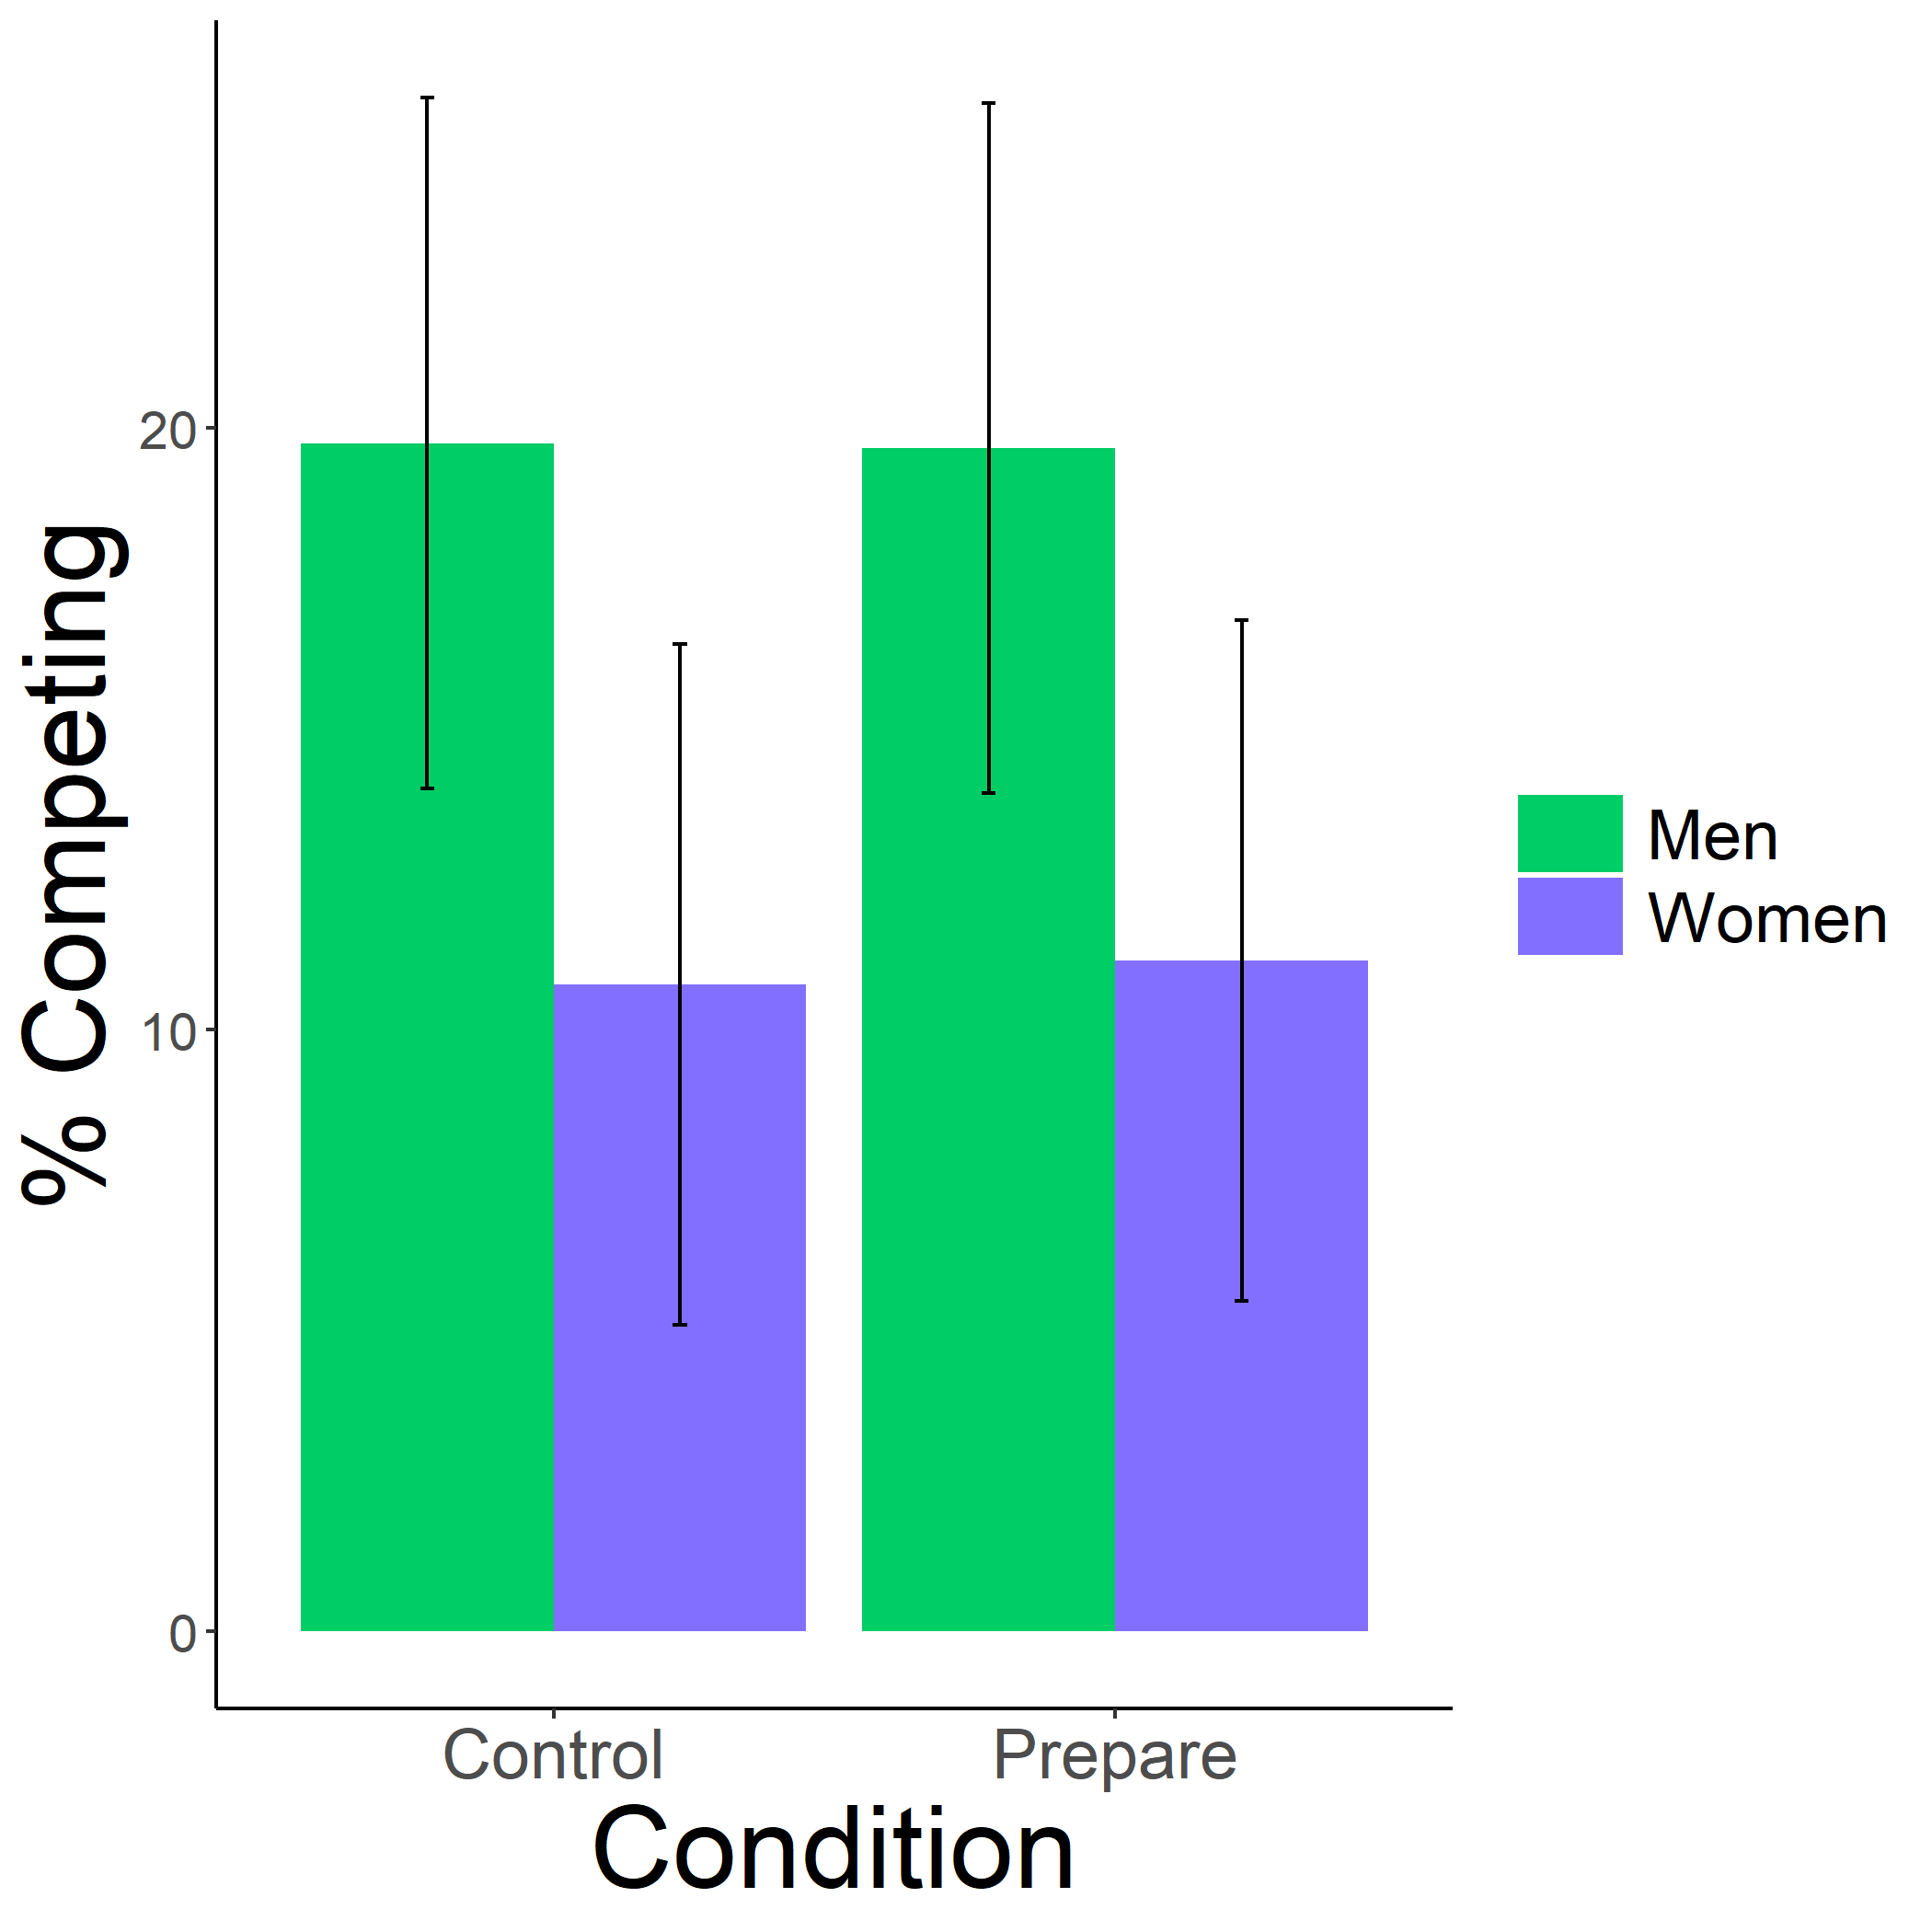
\includegraphics[width=29.17in]{C:/Users/keana/OneDrive - PennO365/Comp_transfer2018/Penn/practice_study/gender-practice/study1/figs/fig00_comp-choice-by-gender-and-cond-bar} \caption{Proportion of male and female participants who chose to compete by condition. We do not find evidence for the hypothesized interaction between gender and condition on the choice to compete, nor do we see a main effect of condition on the choice to compete. Error bars represent standard errors.}\label{fig:s100}
\end{figure}

\begin{figure}
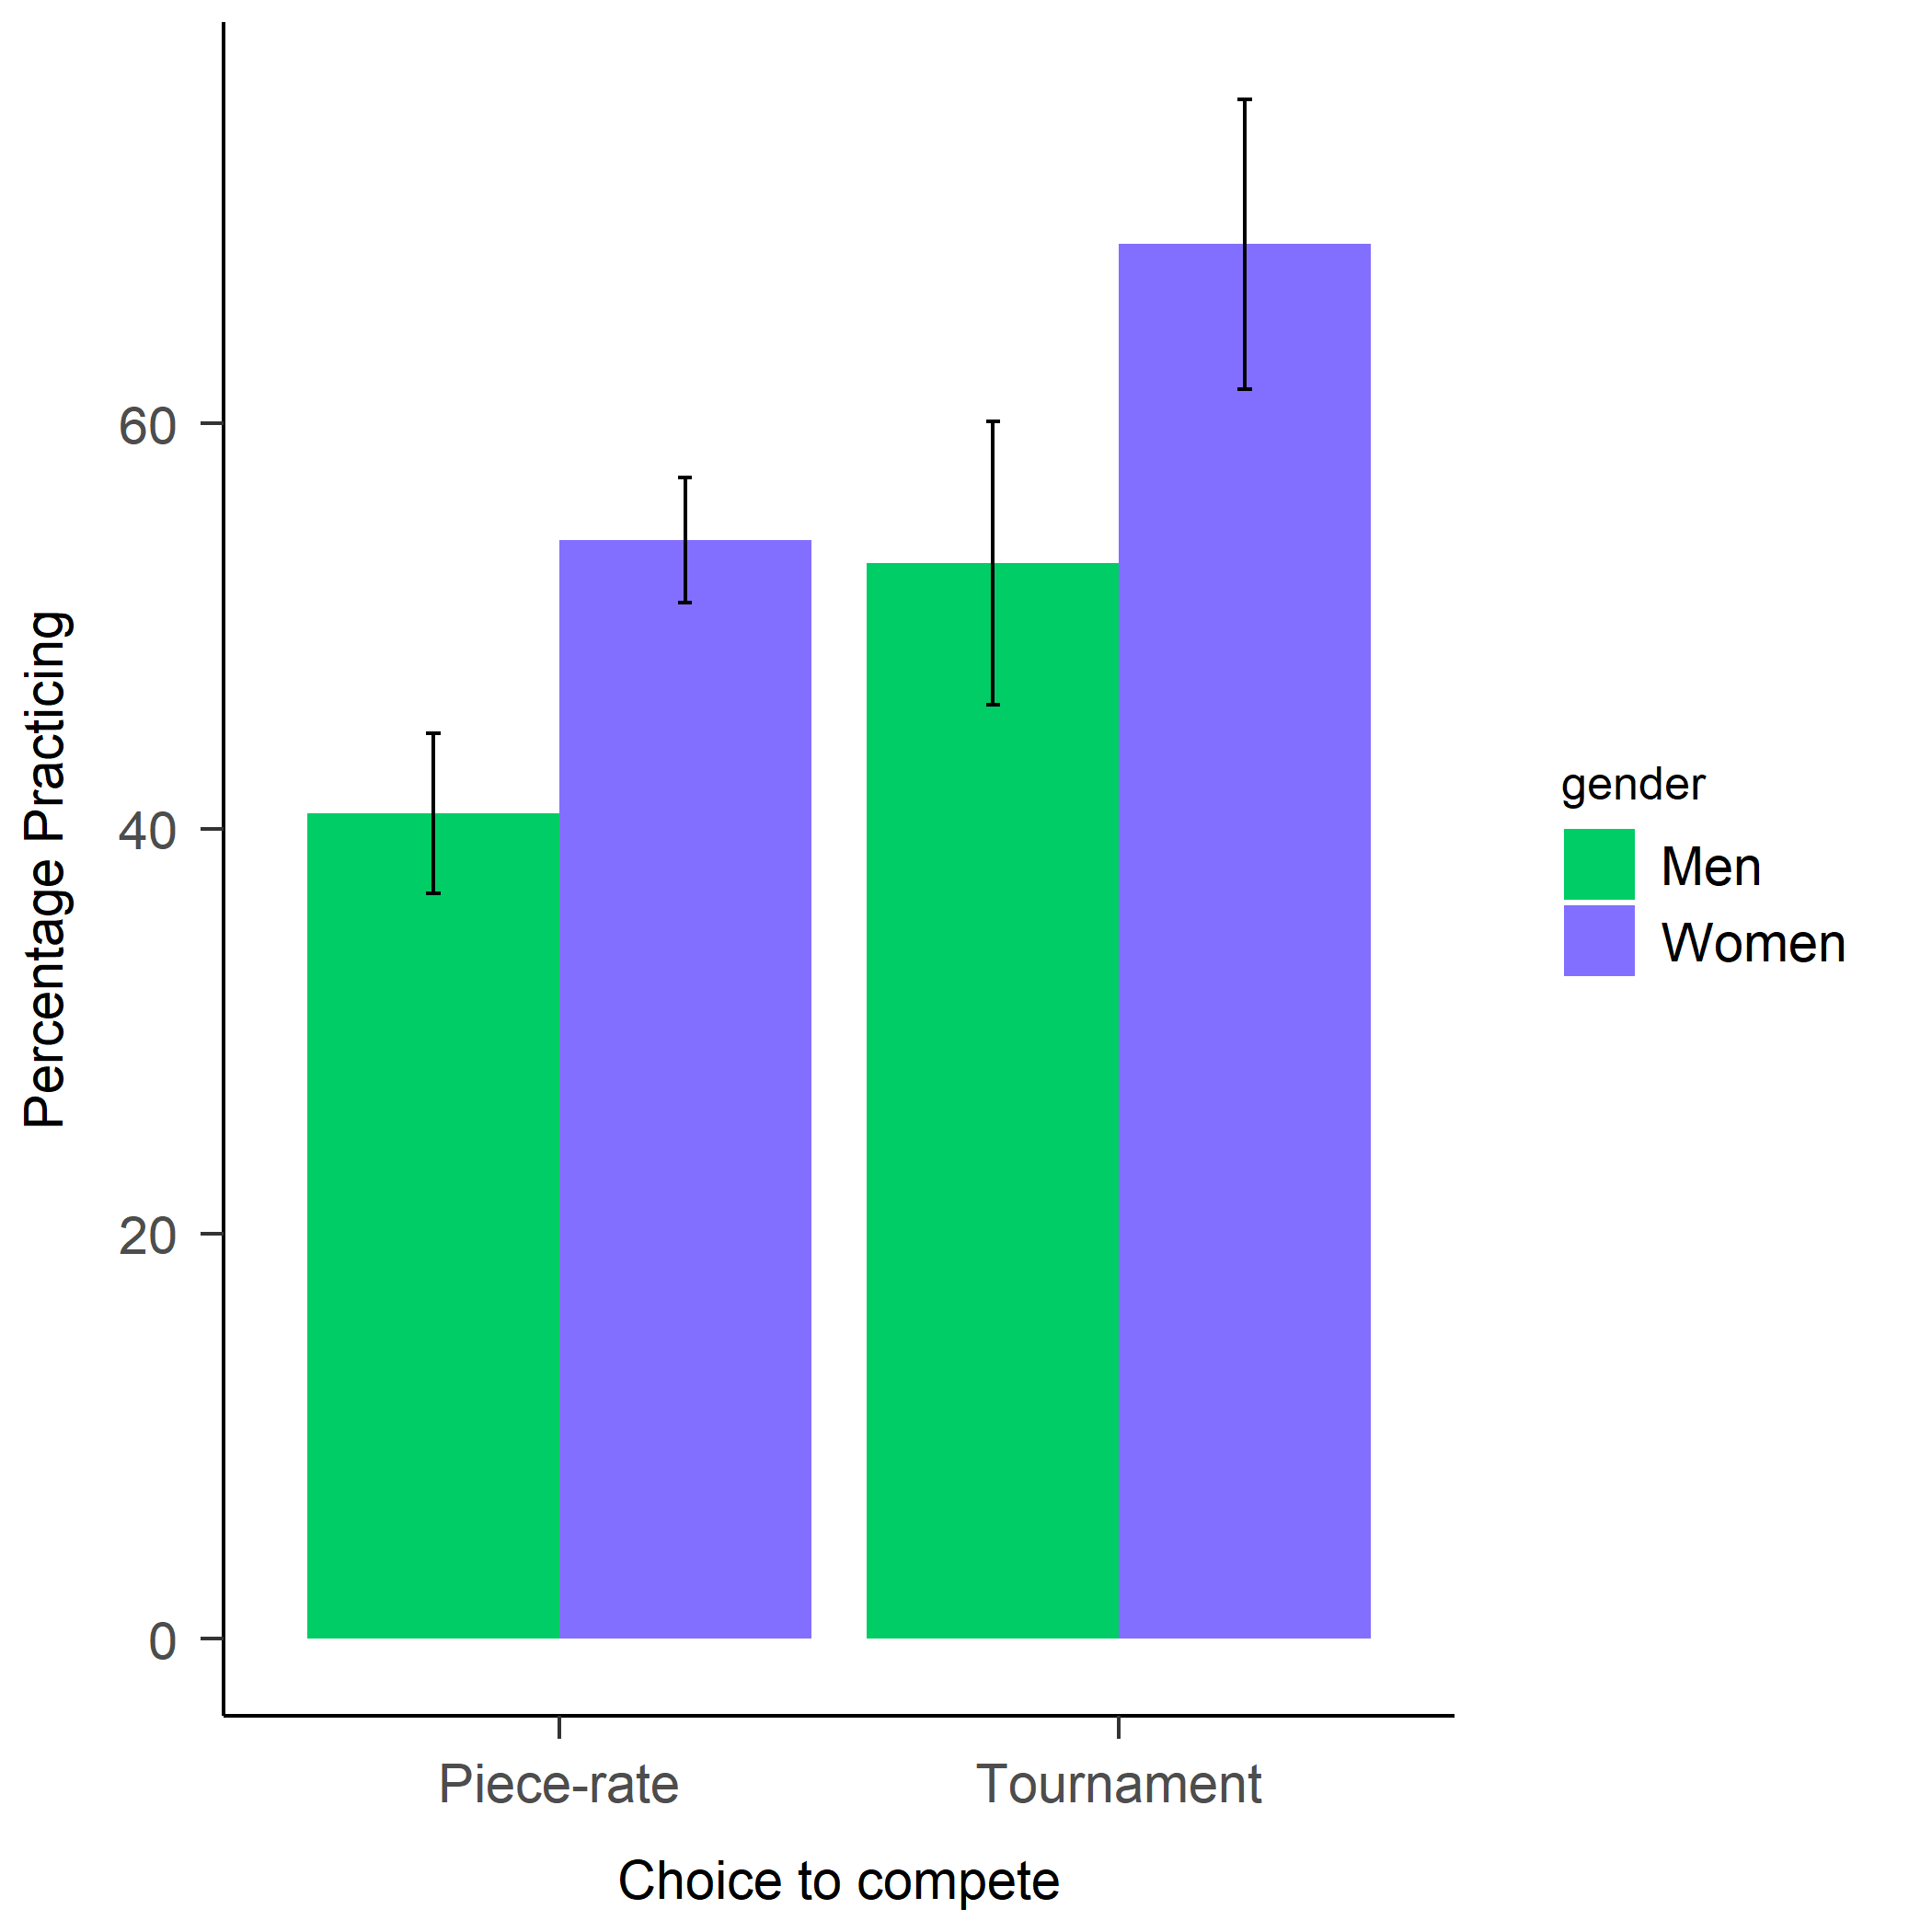
\includegraphics[width=29.17in]{C:/Users/keana/OneDrive - PennO365/Comp_transfer2018/Penn/practice_study/gender-practice/study1/figs/fig01_pract-choice-by-gender-and-comp-choice-bar} \caption{Proportion of male and female participants who chose to prepare by choice to compete. Women are significantly more willing to prepare, even before they know what the preparation involves. There is no interaction between gender and choice to compete on the decision to prepare. Error bars represent standard errors.}\label{fig:s101}
\end{figure}

\begin{figure}
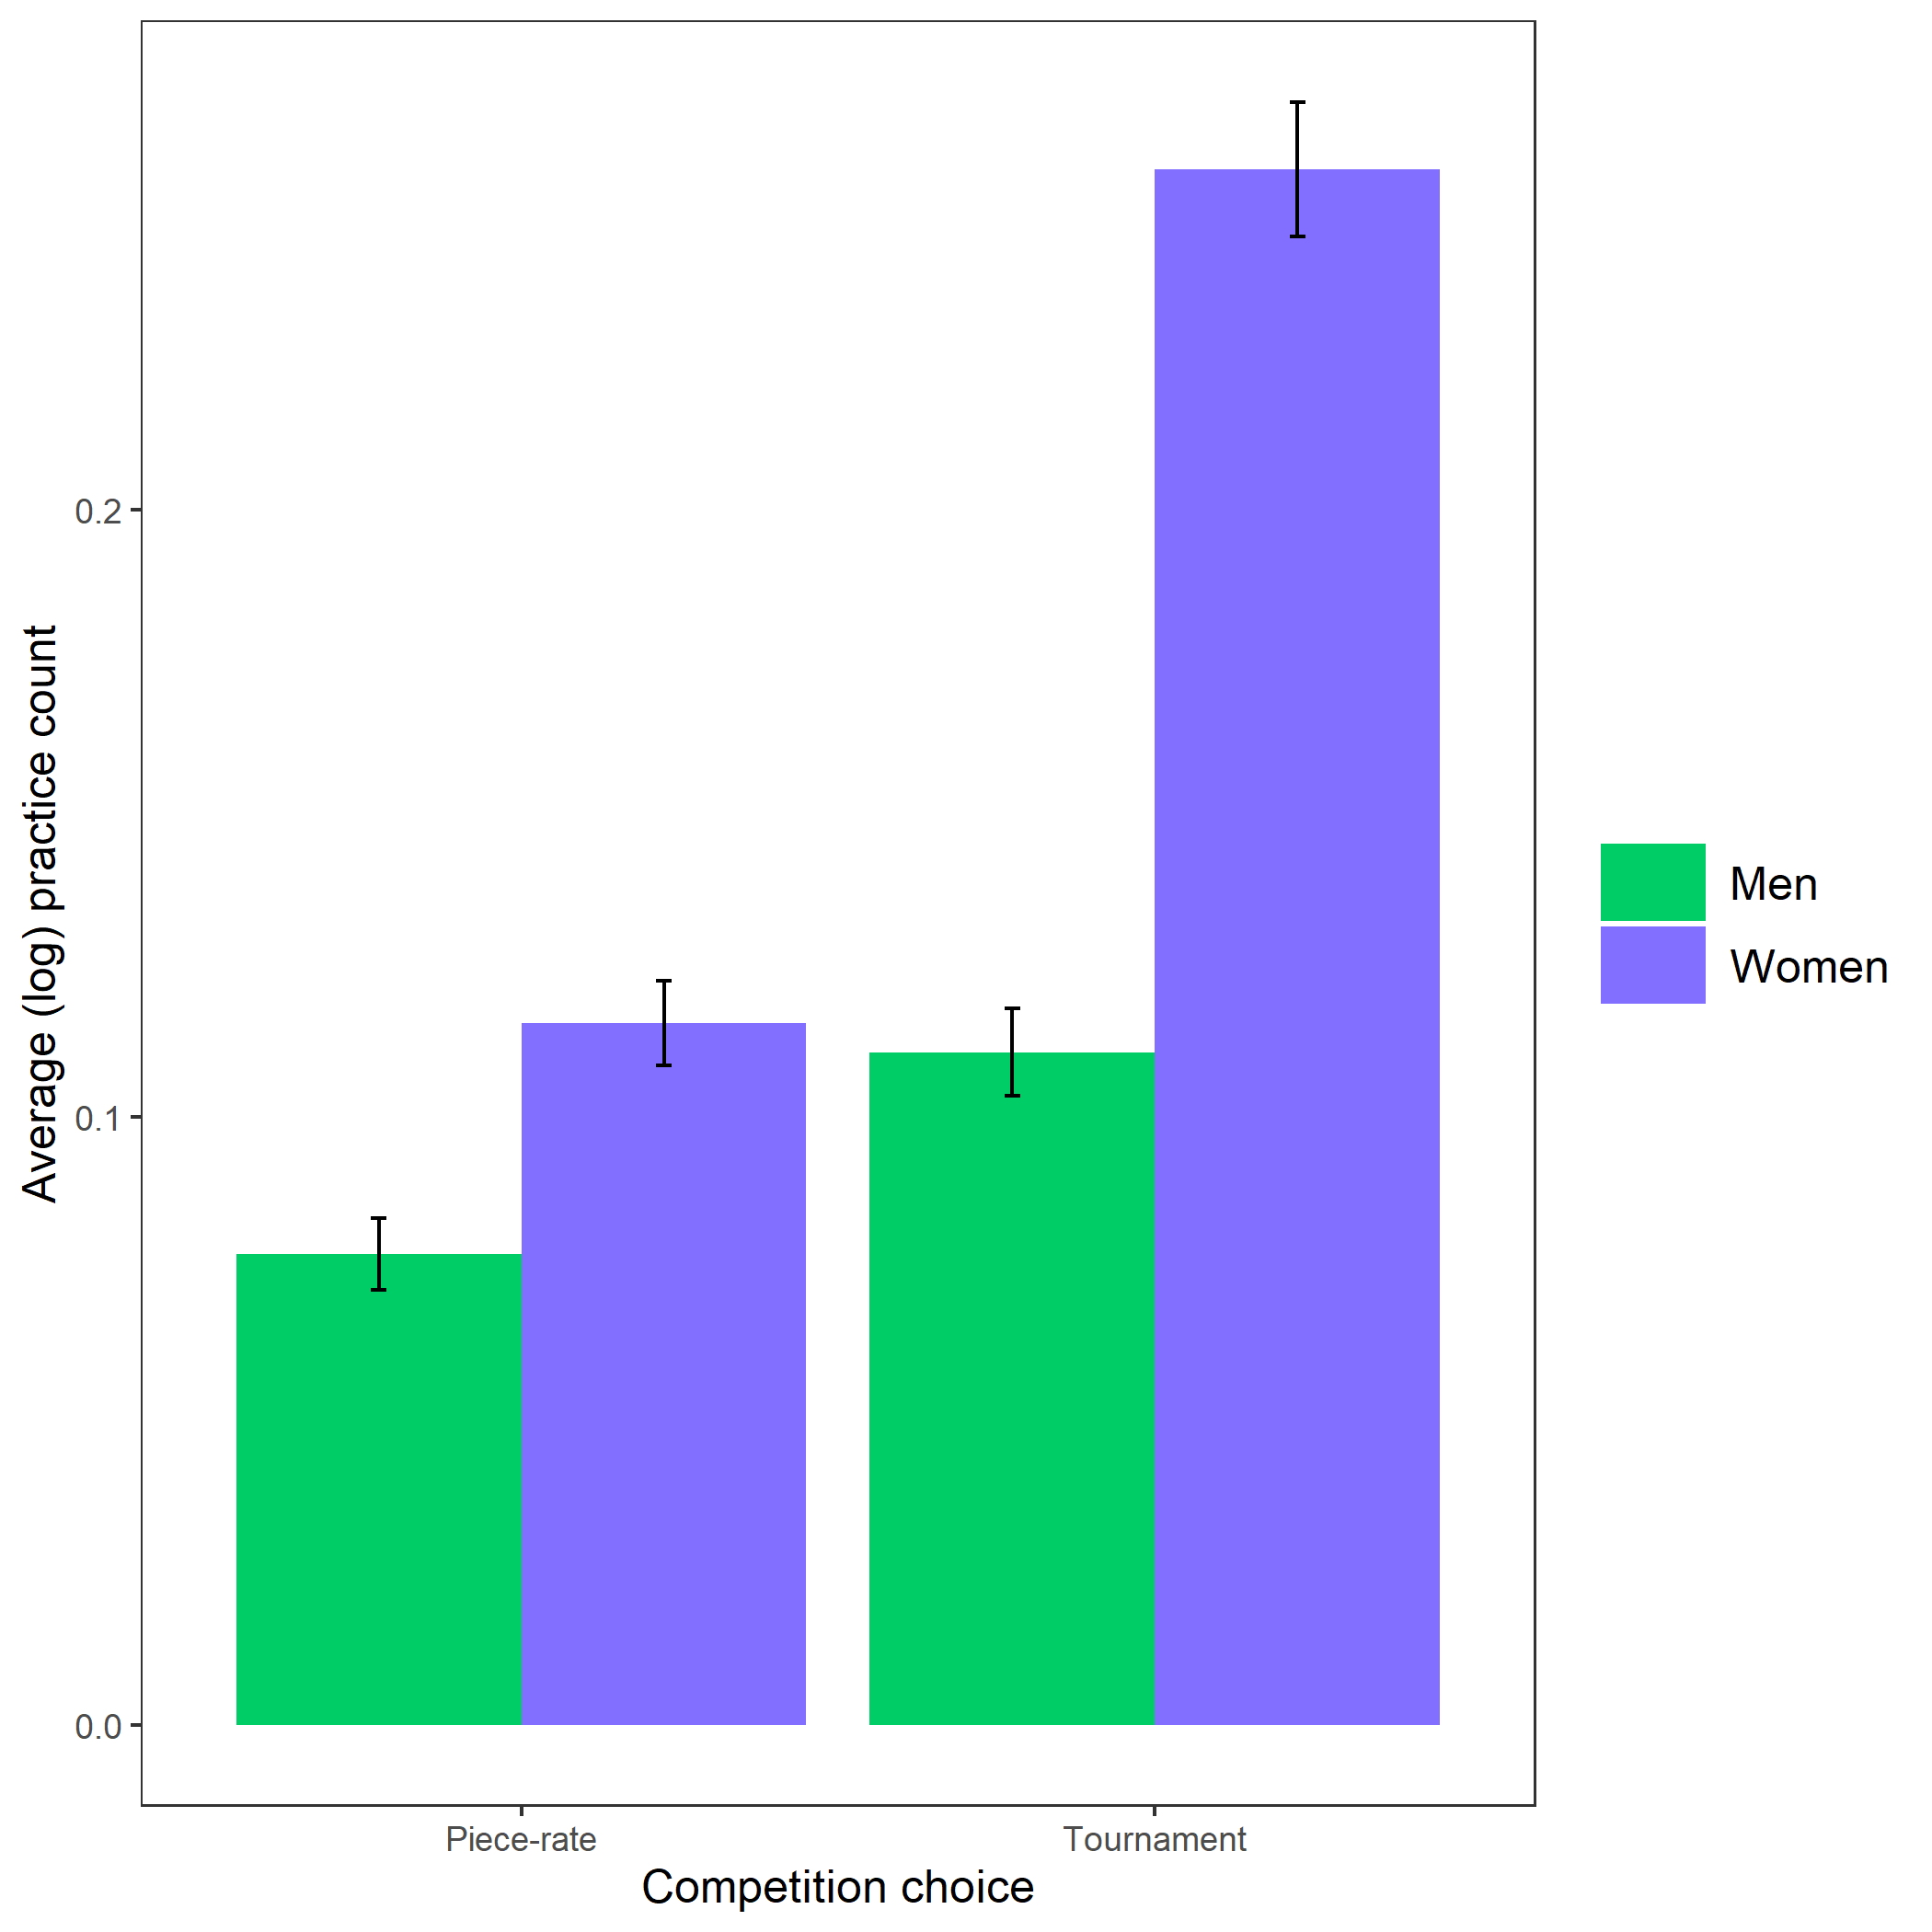
\includegraphics[width=29.17in]{C:/Users/keana/OneDrive - PennO365/Comp_transfer2018/Penn/practice_study/gender-practice/study1/figs/fig02_total-rev-count-by-gender-comp-choice} \caption{Average (log-transformed) practice count based on participant gender and competition choice. We find further evidence of a gender difference in the choice to prepare using a different metric of the choice to prepare: the number of times a participant chooses to persist in their practice effort by repeatedly practicing. Here, we find evidence of a significant interaction between gender and the choice to compete on the choice to practice, where women who chose to compete are significantly more likely to practice. However, the small size of this cell must be considered when interpreting this interaction. Future research is needed to ensure this effect replicates. Error bars represent standard errors.}\label{fig:s102}
\end{figure}

\begin{figure}
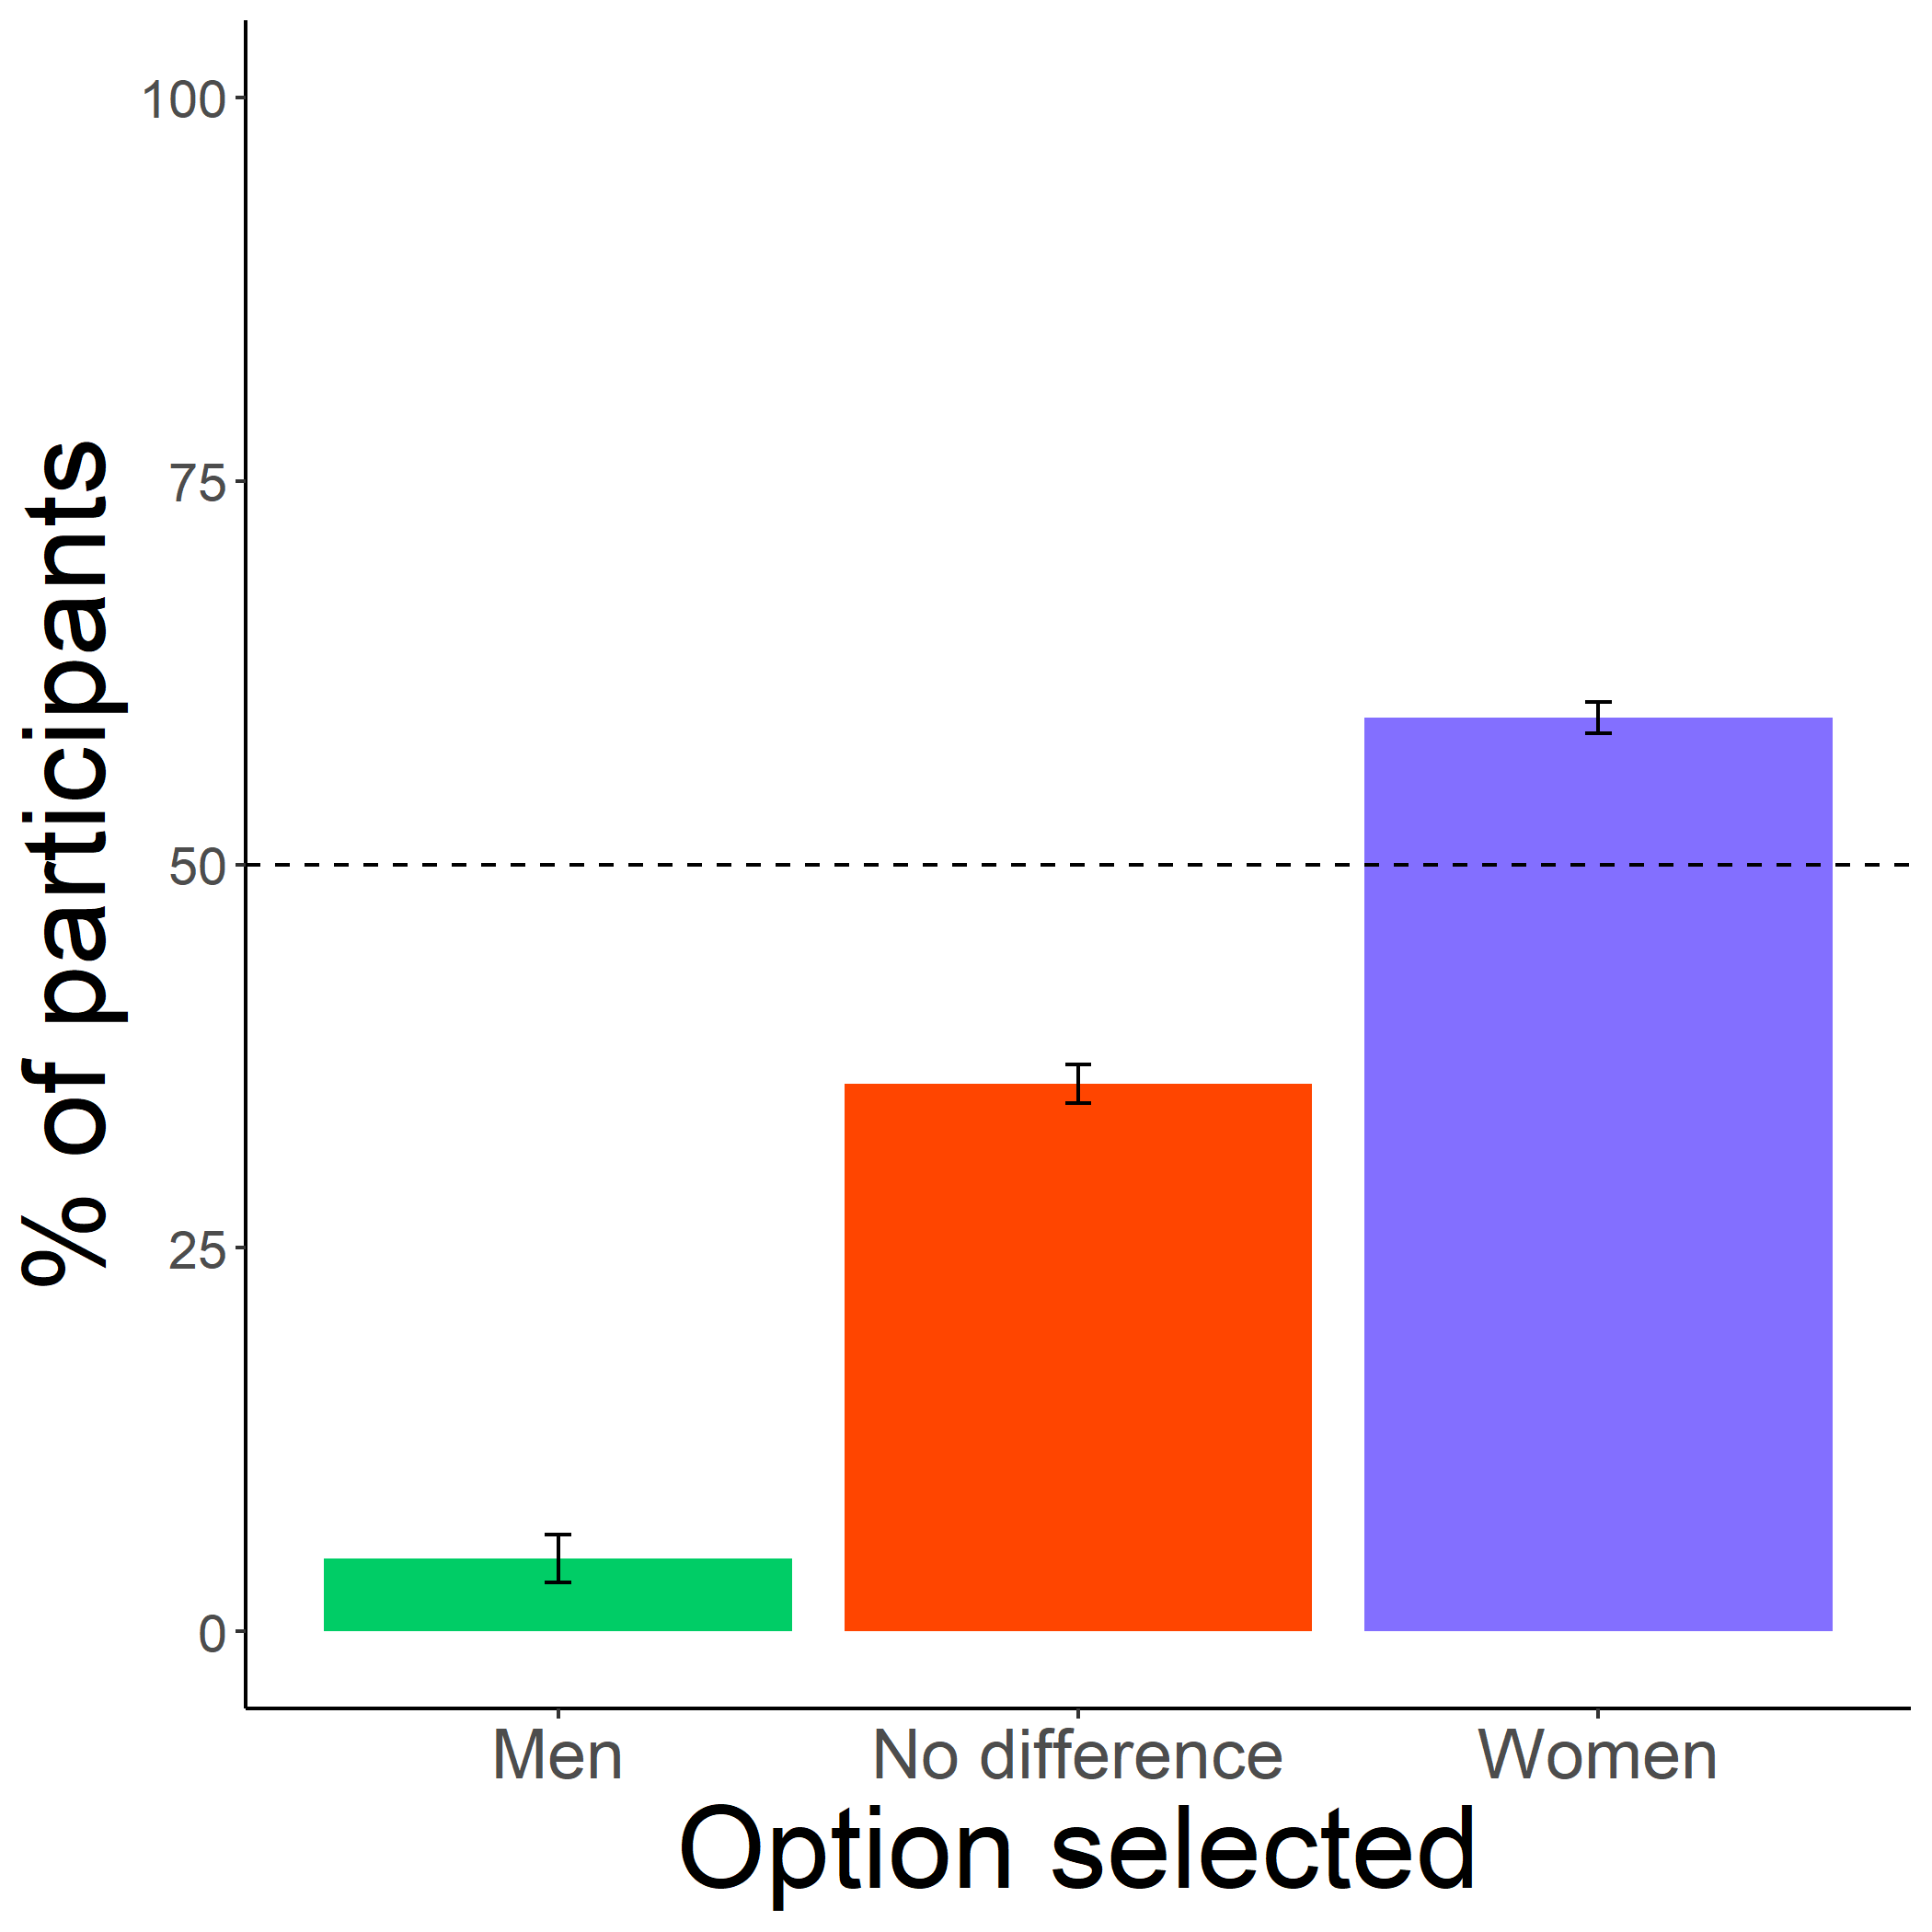
\includegraphics[width=29.17in]{C:/Users/keana/OneDrive - PennO365/Comp_transfer2018/Penn/practice_study/gender-practice/study1/figs/fig03_perc-task-gender-pract} \caption{Participants' perceptions of gender differences in the choice to practice on the task. Both men and women correctly anticipate that women will be more willing to practice before completing the multiplication task. Women are especially likely to state women will prepare more for the task. Error bars represent standard errors.}\label{fig:s103}
\end{figure}

\begin{figure}
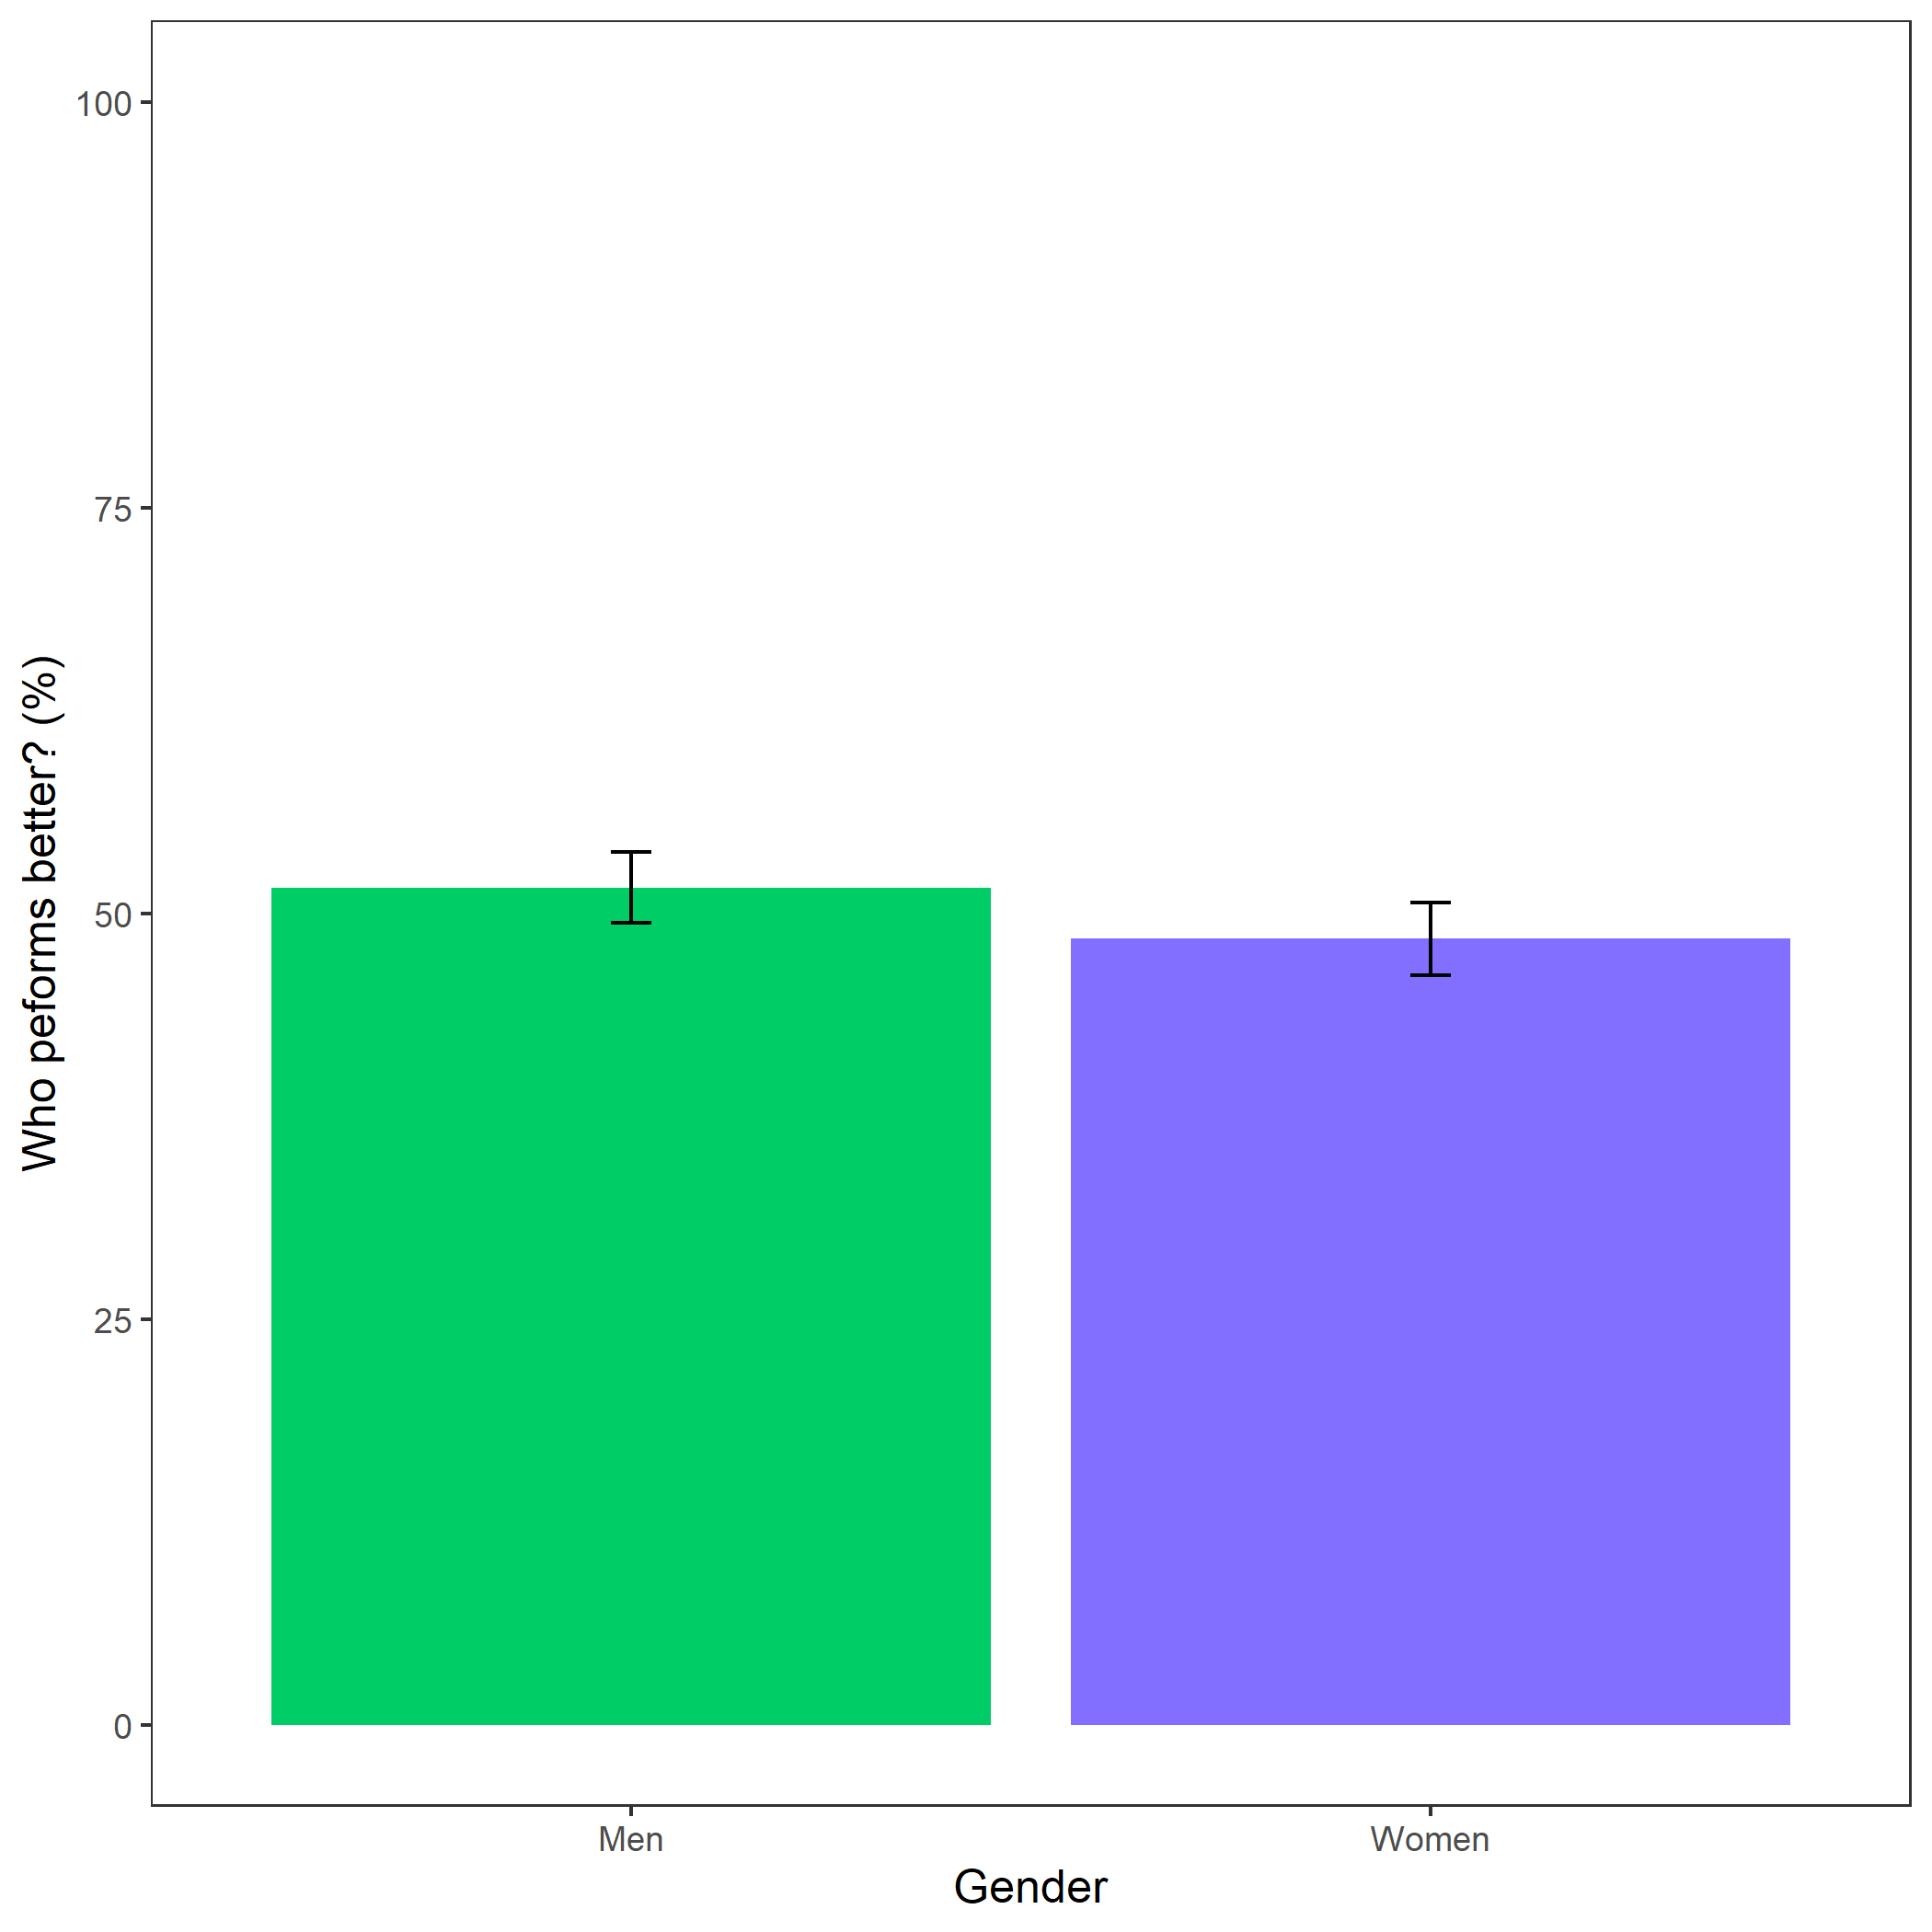
\includegraphics[width=29.17in]{C:/Users/keana/OneDrive - PennO365/Comp_transfer2018/Penn/practice_study/gender-practice/study1/figs/fig04_better-gender-guess} \caption{Participants' perceptions of gender differences in performance on the task. Participants were equally likely to predict that women (vs. men) would perform better on the task, suggesting that participants did not have strong stereotypes about gender differences in performance on the multiplication task. Error bars represent standard errors.}\label{fig:s104}
\end{figure}

\begin{figure}
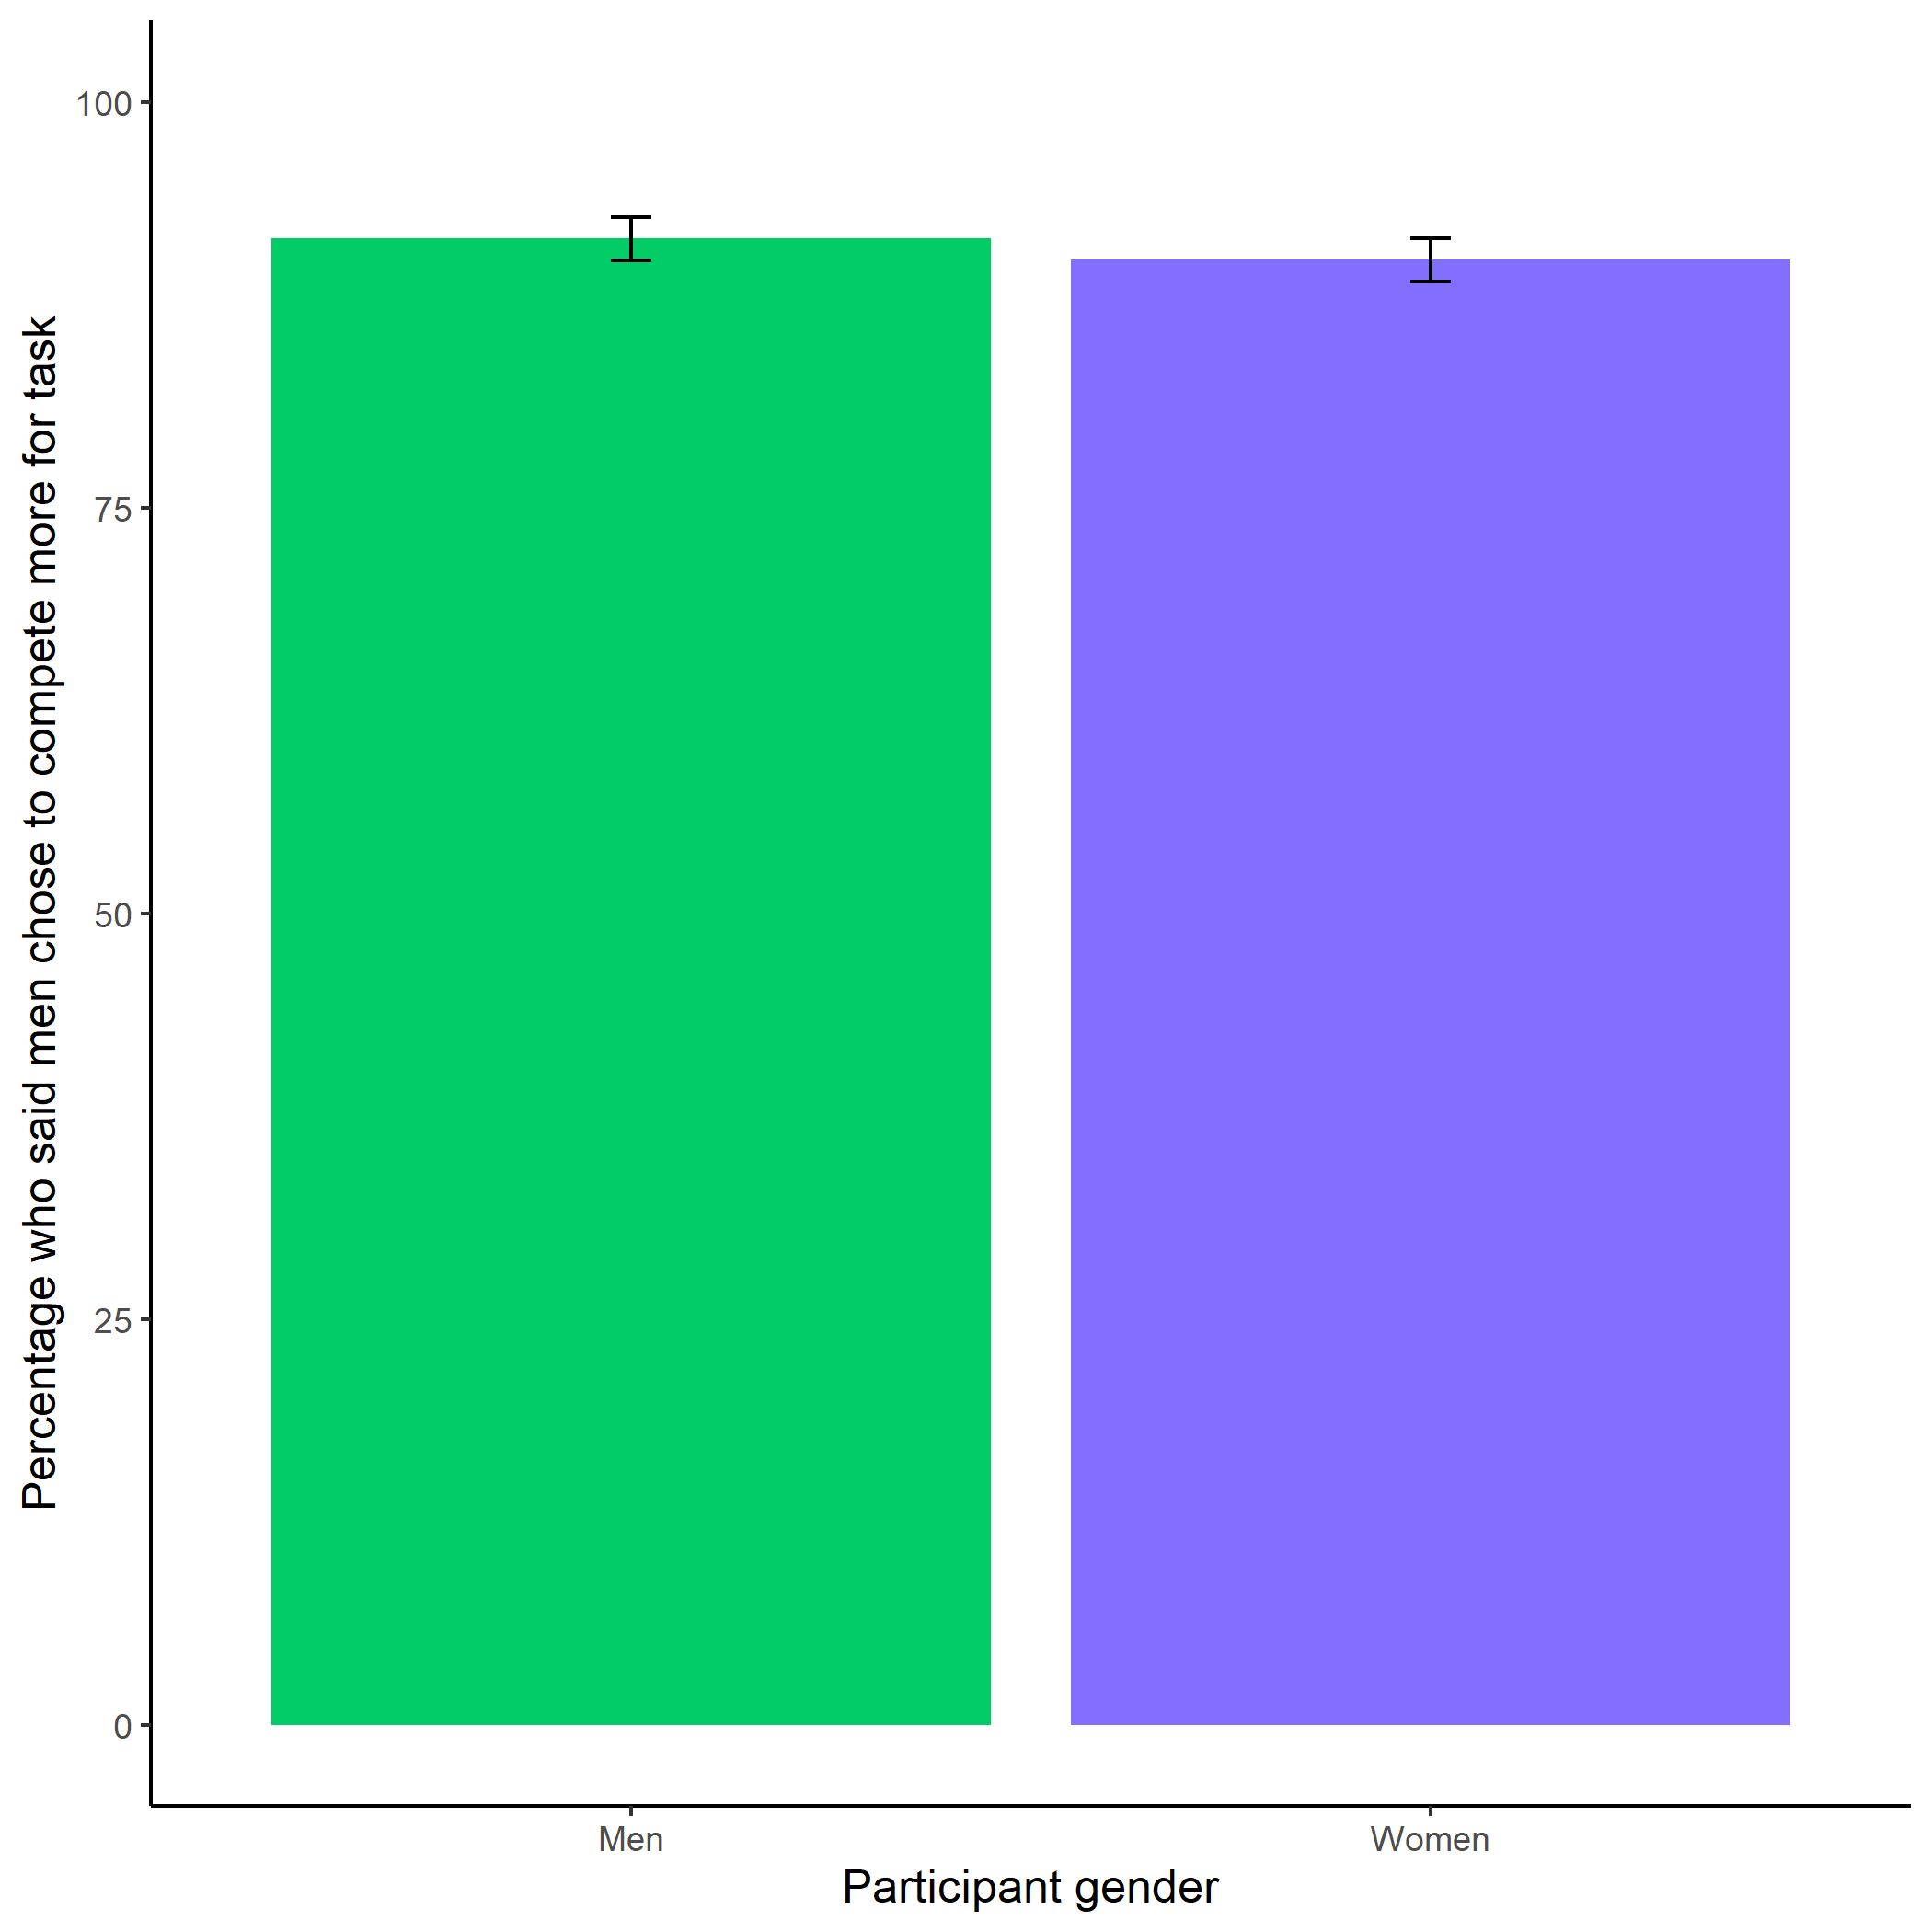
\includegraphics[width=29.17in]{C:/Users/keana/OneDrive - PennO365/Comp_transfer2018/Penn/practice_study/gender-practice/study1/figs/fig05_perc-gender-comp} \caption{Participants' perceptions of gender differences in choice to compete. Both men and women were significantly more likely than chance to correctly state that men would be more likely to choose to compete during the multiplication task, suggesting strong stereotypes about gender differences in competitiveness. Error bars represent standard errors.}\label{fig:s105}
\end{figure}

\begin{figure}
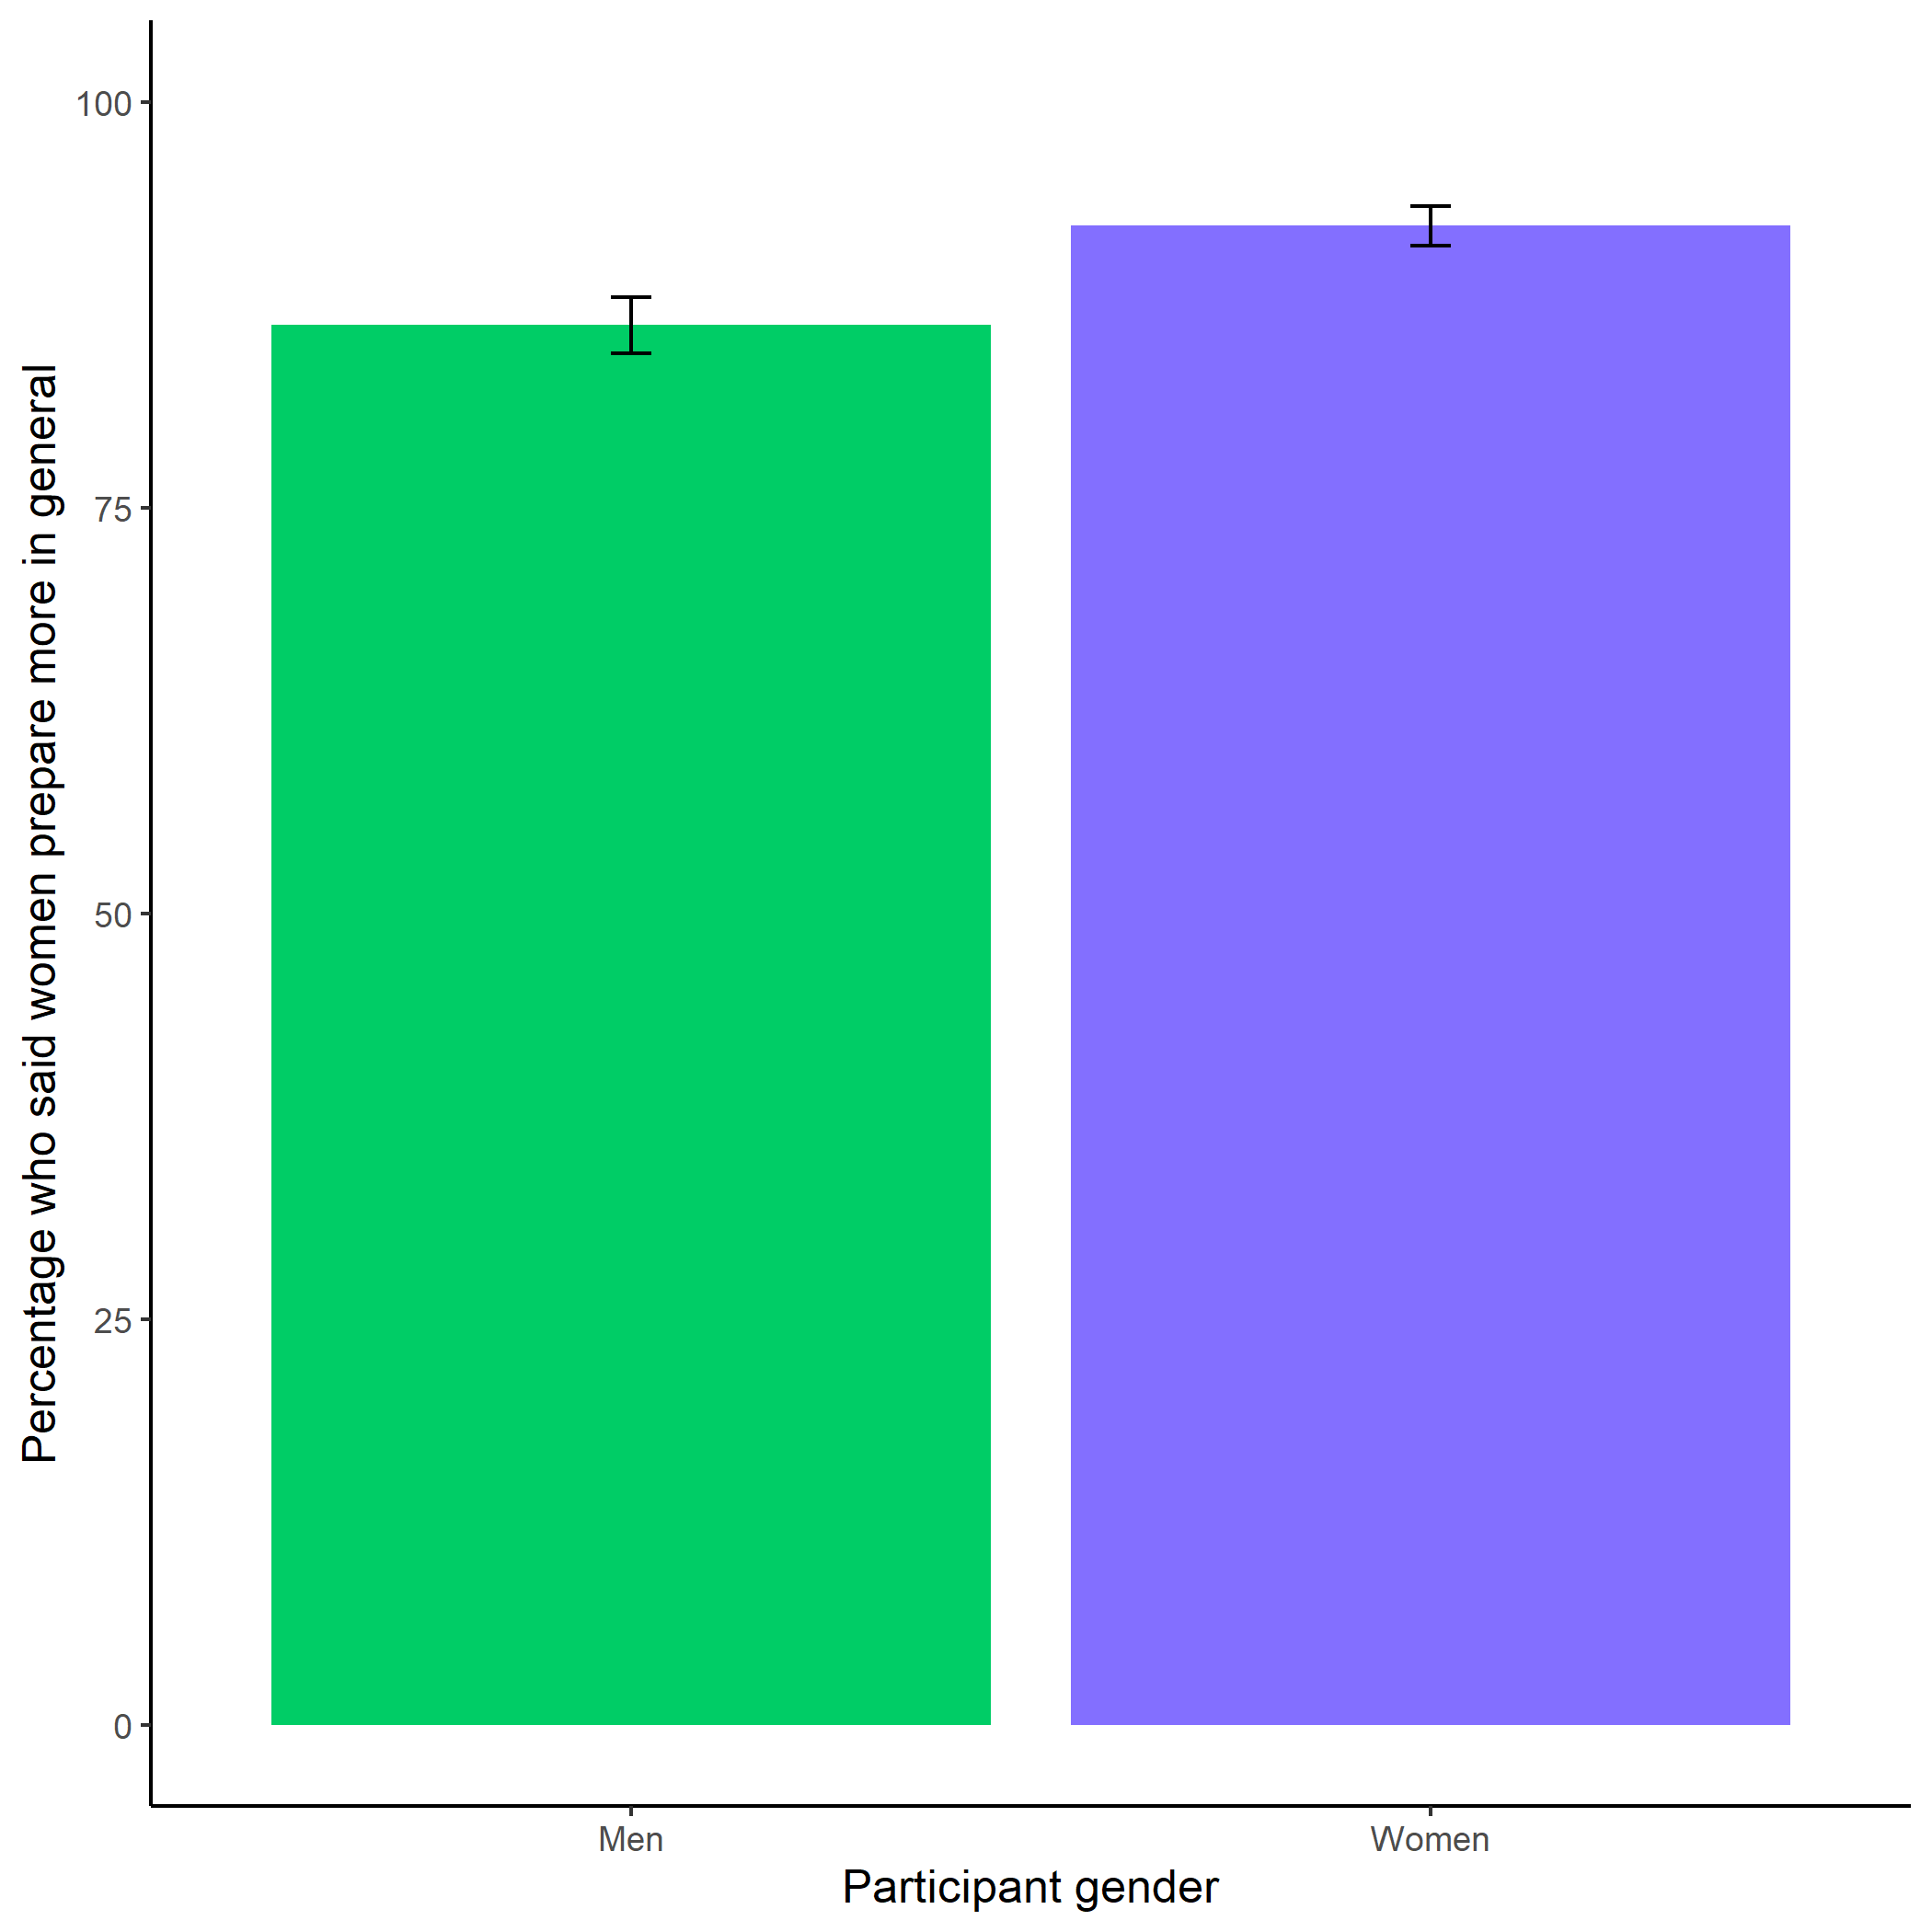
\includegraphics[width=29.17in]{C:/Users/keana/OneDrive - PennO365/Comp_transfer2018/Penn/practice_study/gender-practice/study1/figs/fig06_perc-gen-gender-pract} \caption{Participants' perceptions of general gender differences in choice to practice. Both men and women (but especially women) were significantly more likely than chance to say that women prepare more in general than men. Again, these findings suggest that participants observe these gender differences directly or are aware of stereotypes about gender differences in the choice to prepare. Error bars represent standard errors.}\label{fig:s106}
\end{figure}

\hypertarget{study-2-1}{%
\section{Study 2}\label{study-2-1}}

\begin{figure}
\includegraphics[width=29.17in]{C:/Users/keana/OneDrive - PennO365/Comp_transfer2018/Penn/practice_study/gender-practice/study2/figs/fig00_comp-choice-women-by-cond} \caption{Proportion of female participants who chose to compete by condition. We do not find evidence of the hypothesized effect of condition on the choice to compete, there were no significant differences in entry into competition between women in the control vs. prepare conditions. Error bars represent standard errors.}\label{fig:s200}
\end{figure}

\begin{figure}
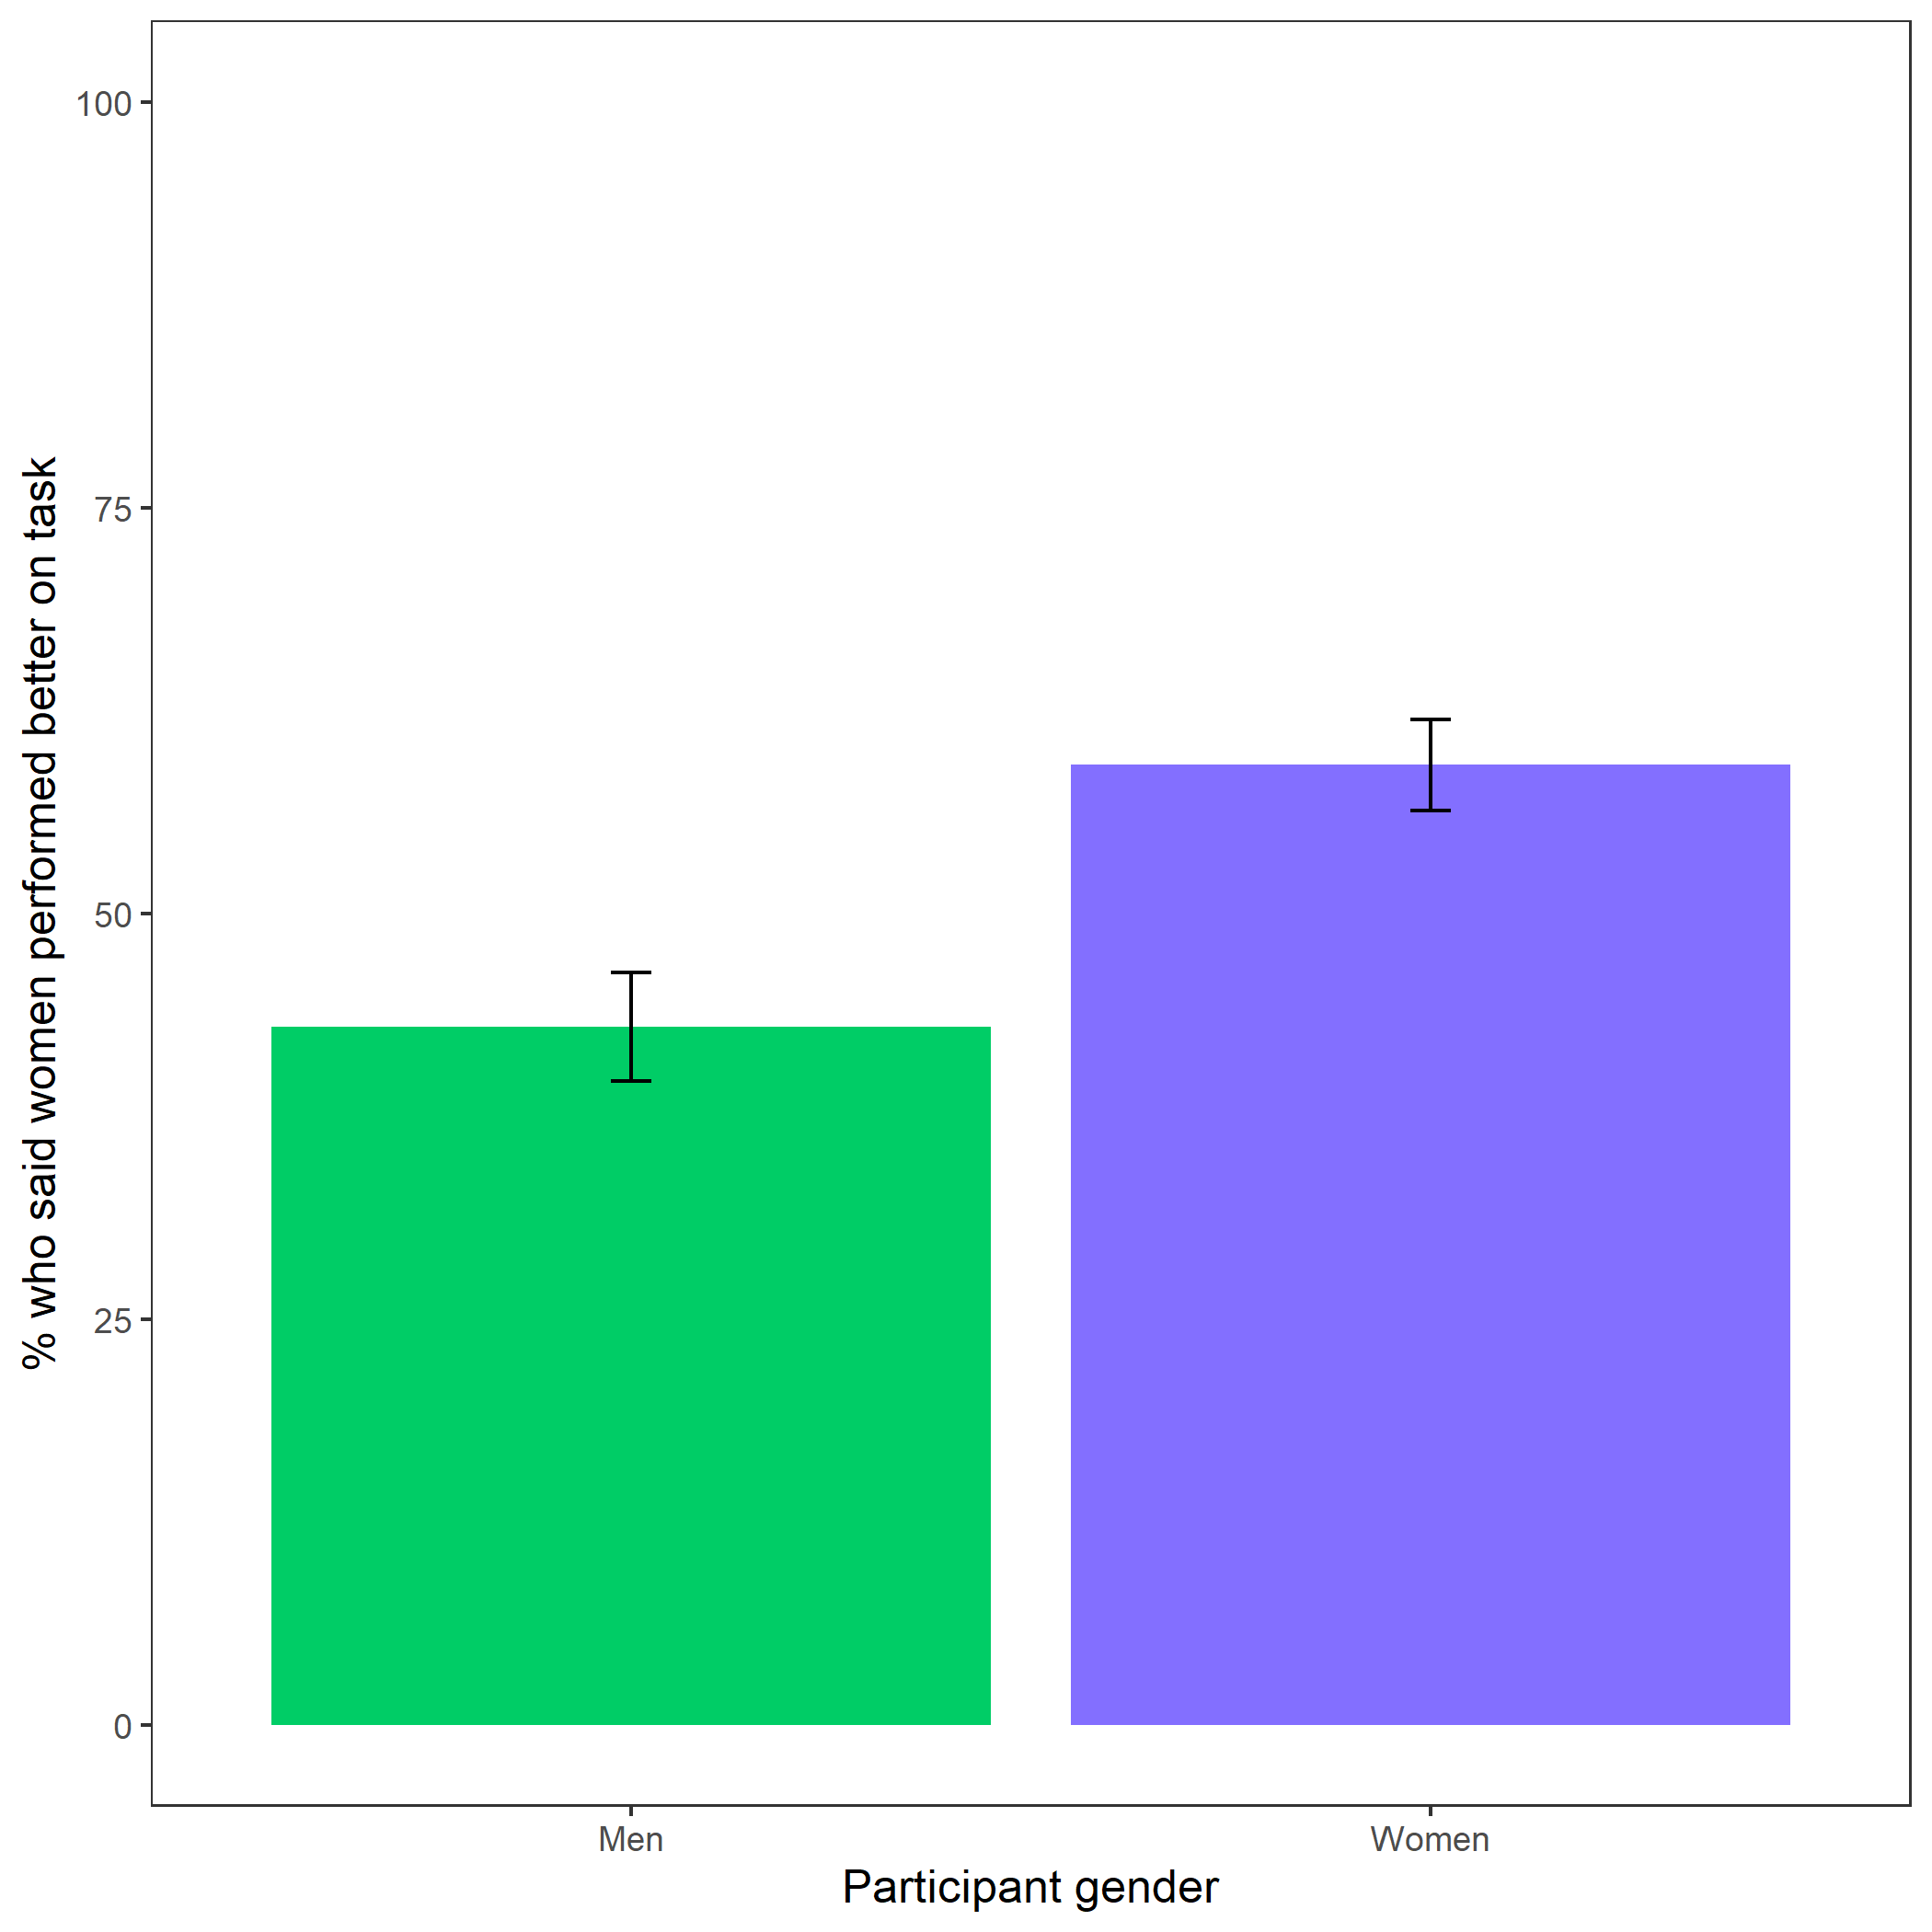
\includegraphics[width=29.17in]{C:/Users/keana/OneDrive - PennO365/Comp_transfer2018/Penn/practice_study/gender-practice/study2/figs/fig01_better-gender-guess} \caption{Participants' perceptions of gender differences in performance on the task. We replicate the effect from Study 1, where participants were not significantly more likely than chance to anticipate that one gender would perform better on the task. Error bars represent standard errors.}\label{fig:s201}
\end{figure}

\begin{figure}
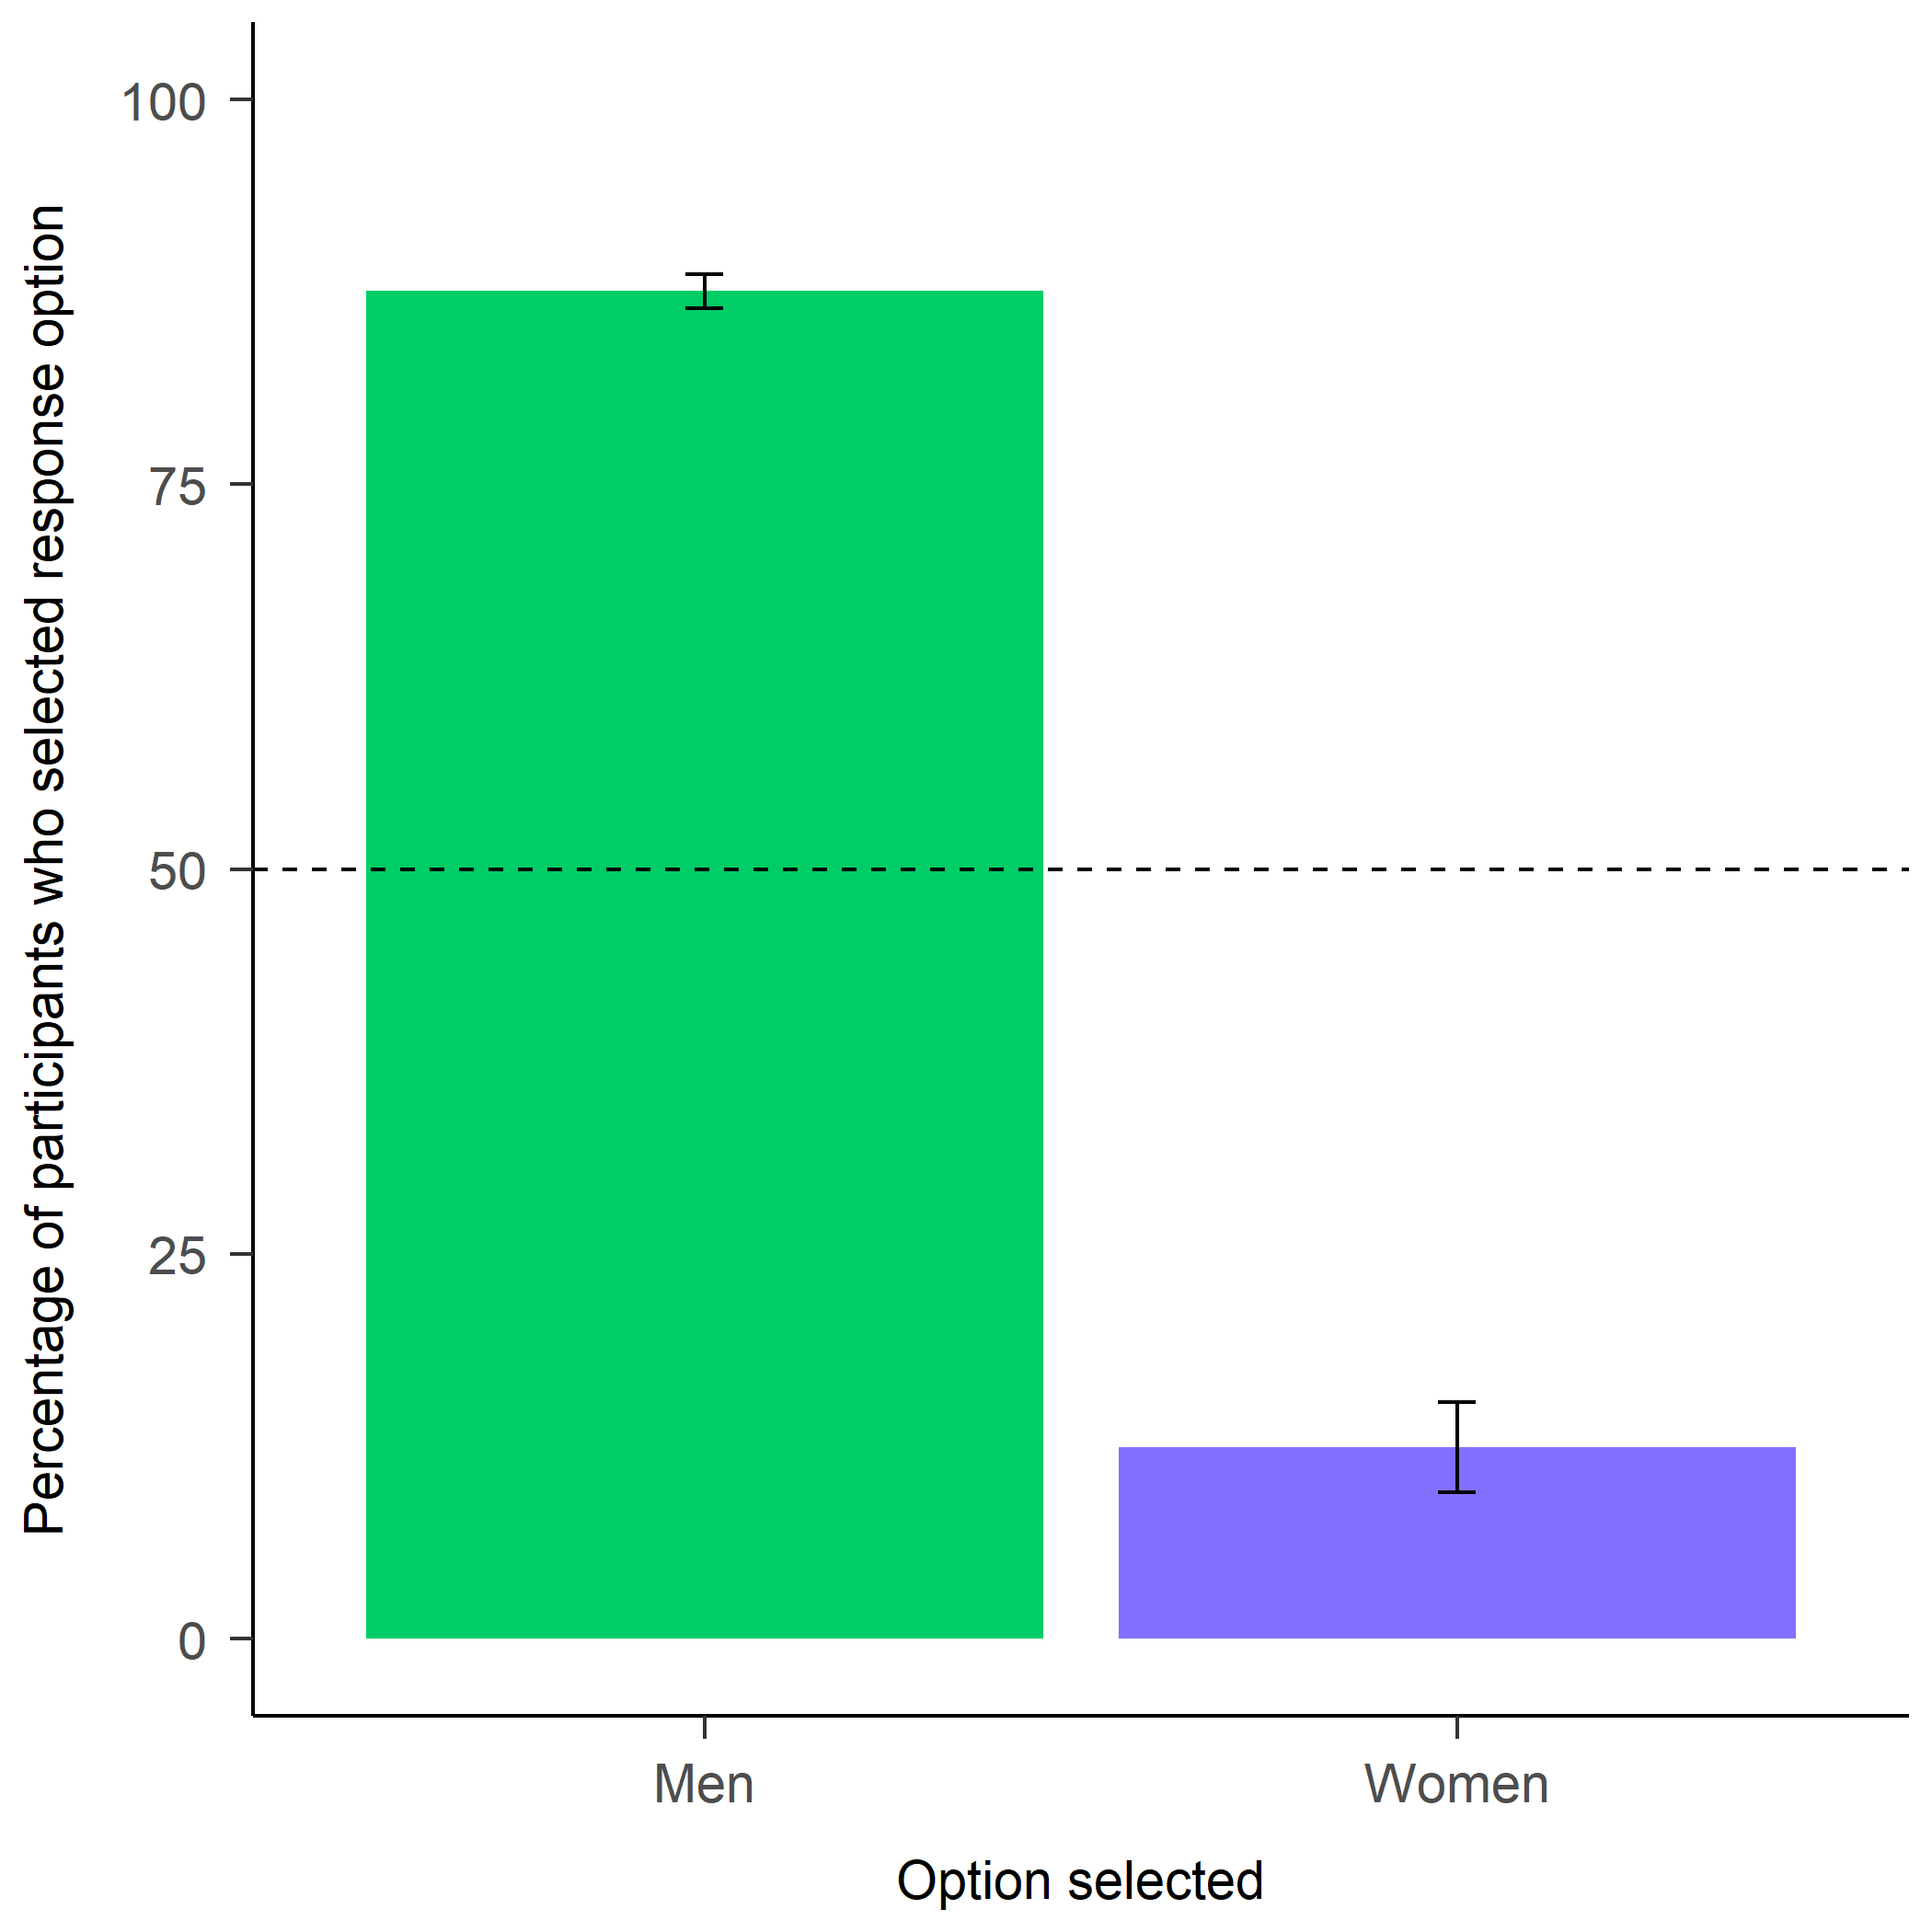
\includegraphics[width=29.17in]{C:/Users/keana/OneDrive - PennO365/Comp_transfer2018/Penn/practice_study/gender-practice/study2/figs/fig02_perc-gender-comp} \caption{Participants' perceptions of gender differences in choice to compete. Replicating the finding from Study 1, participants (especially men) in Study 2 are significantly more likely than chance to state that men chose the competitive payment scheme. Error bars represent standard errors.}\label{fig:s202}
\end{figure}

\begin{figure}
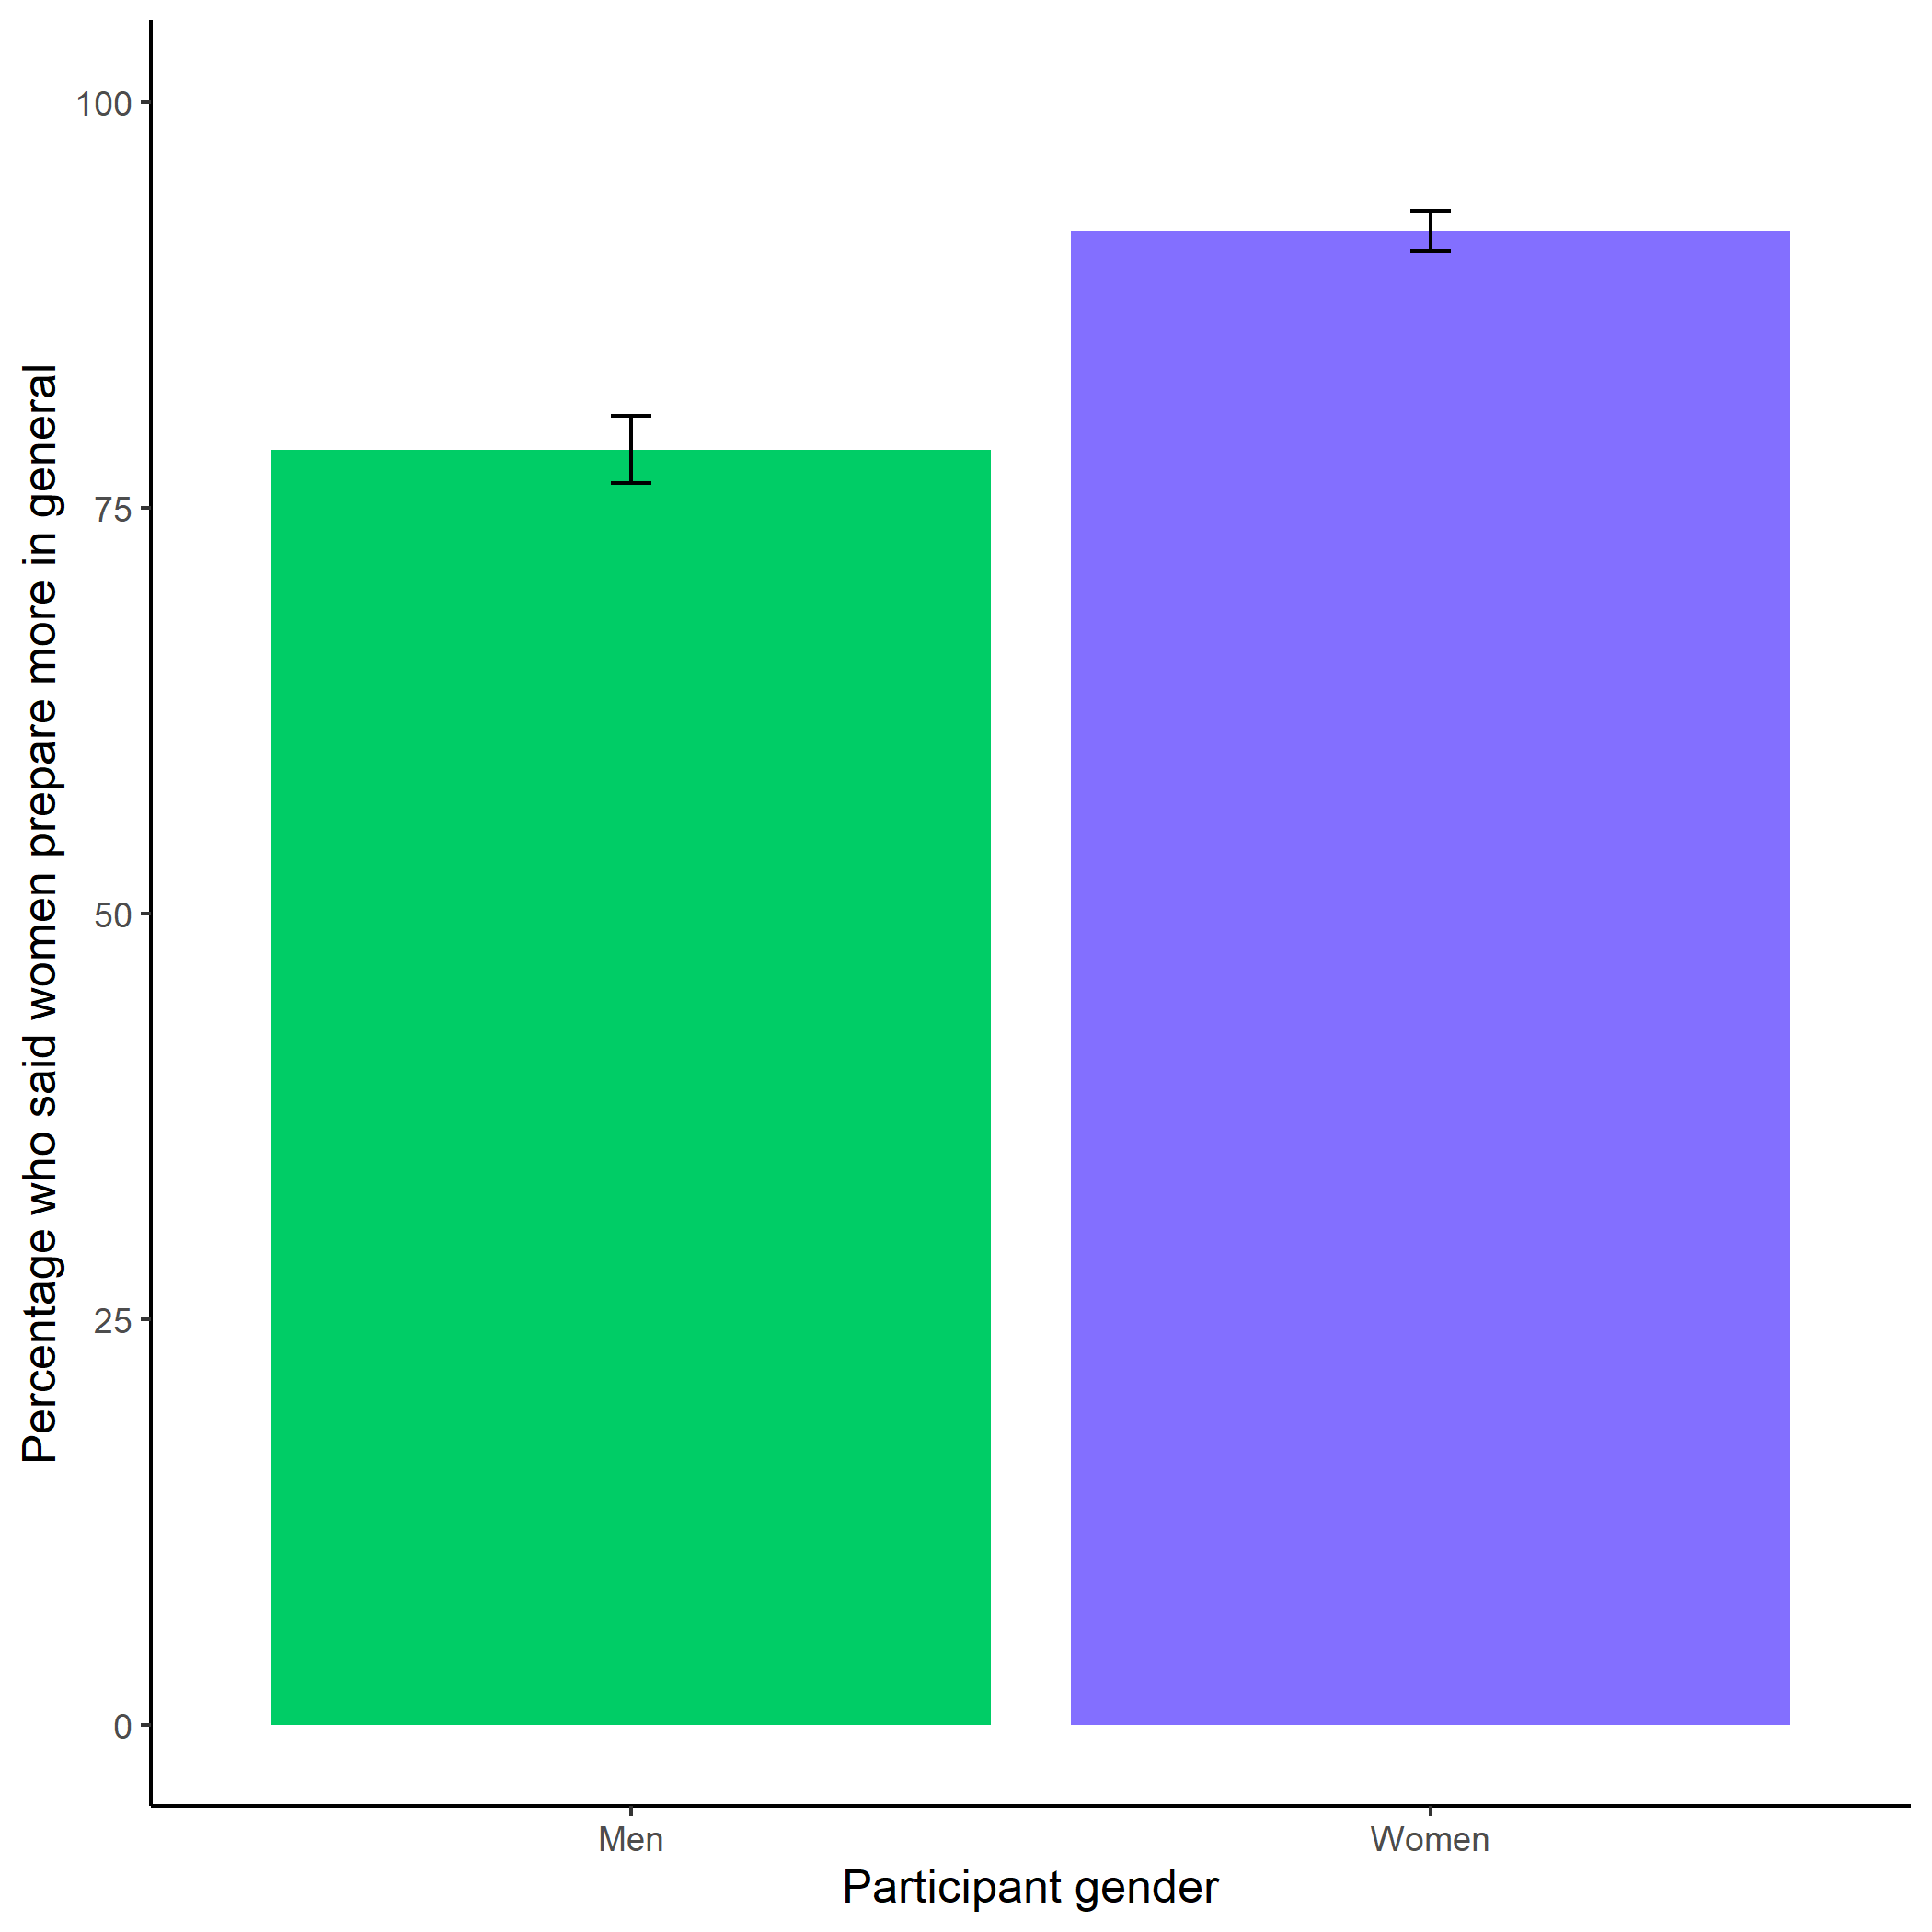
\includegraphics[width=29.17in]{C:/Users/keana/OneDrive - PennO365/Comp_transfer2018/Penn/practice_study/gender-practice/study2/figs/fig03_perc-gen-gender-pract} \caption{Participants' perceptions of general gender differences in choice to prepare. We replicate the findings from Study 1, where participants (especially women) are significantly more likely than chance to state that women prepare more in general than men. Error bars represent standard errors.}\label{fig:s203}
\end{figure}

\begin{figure}
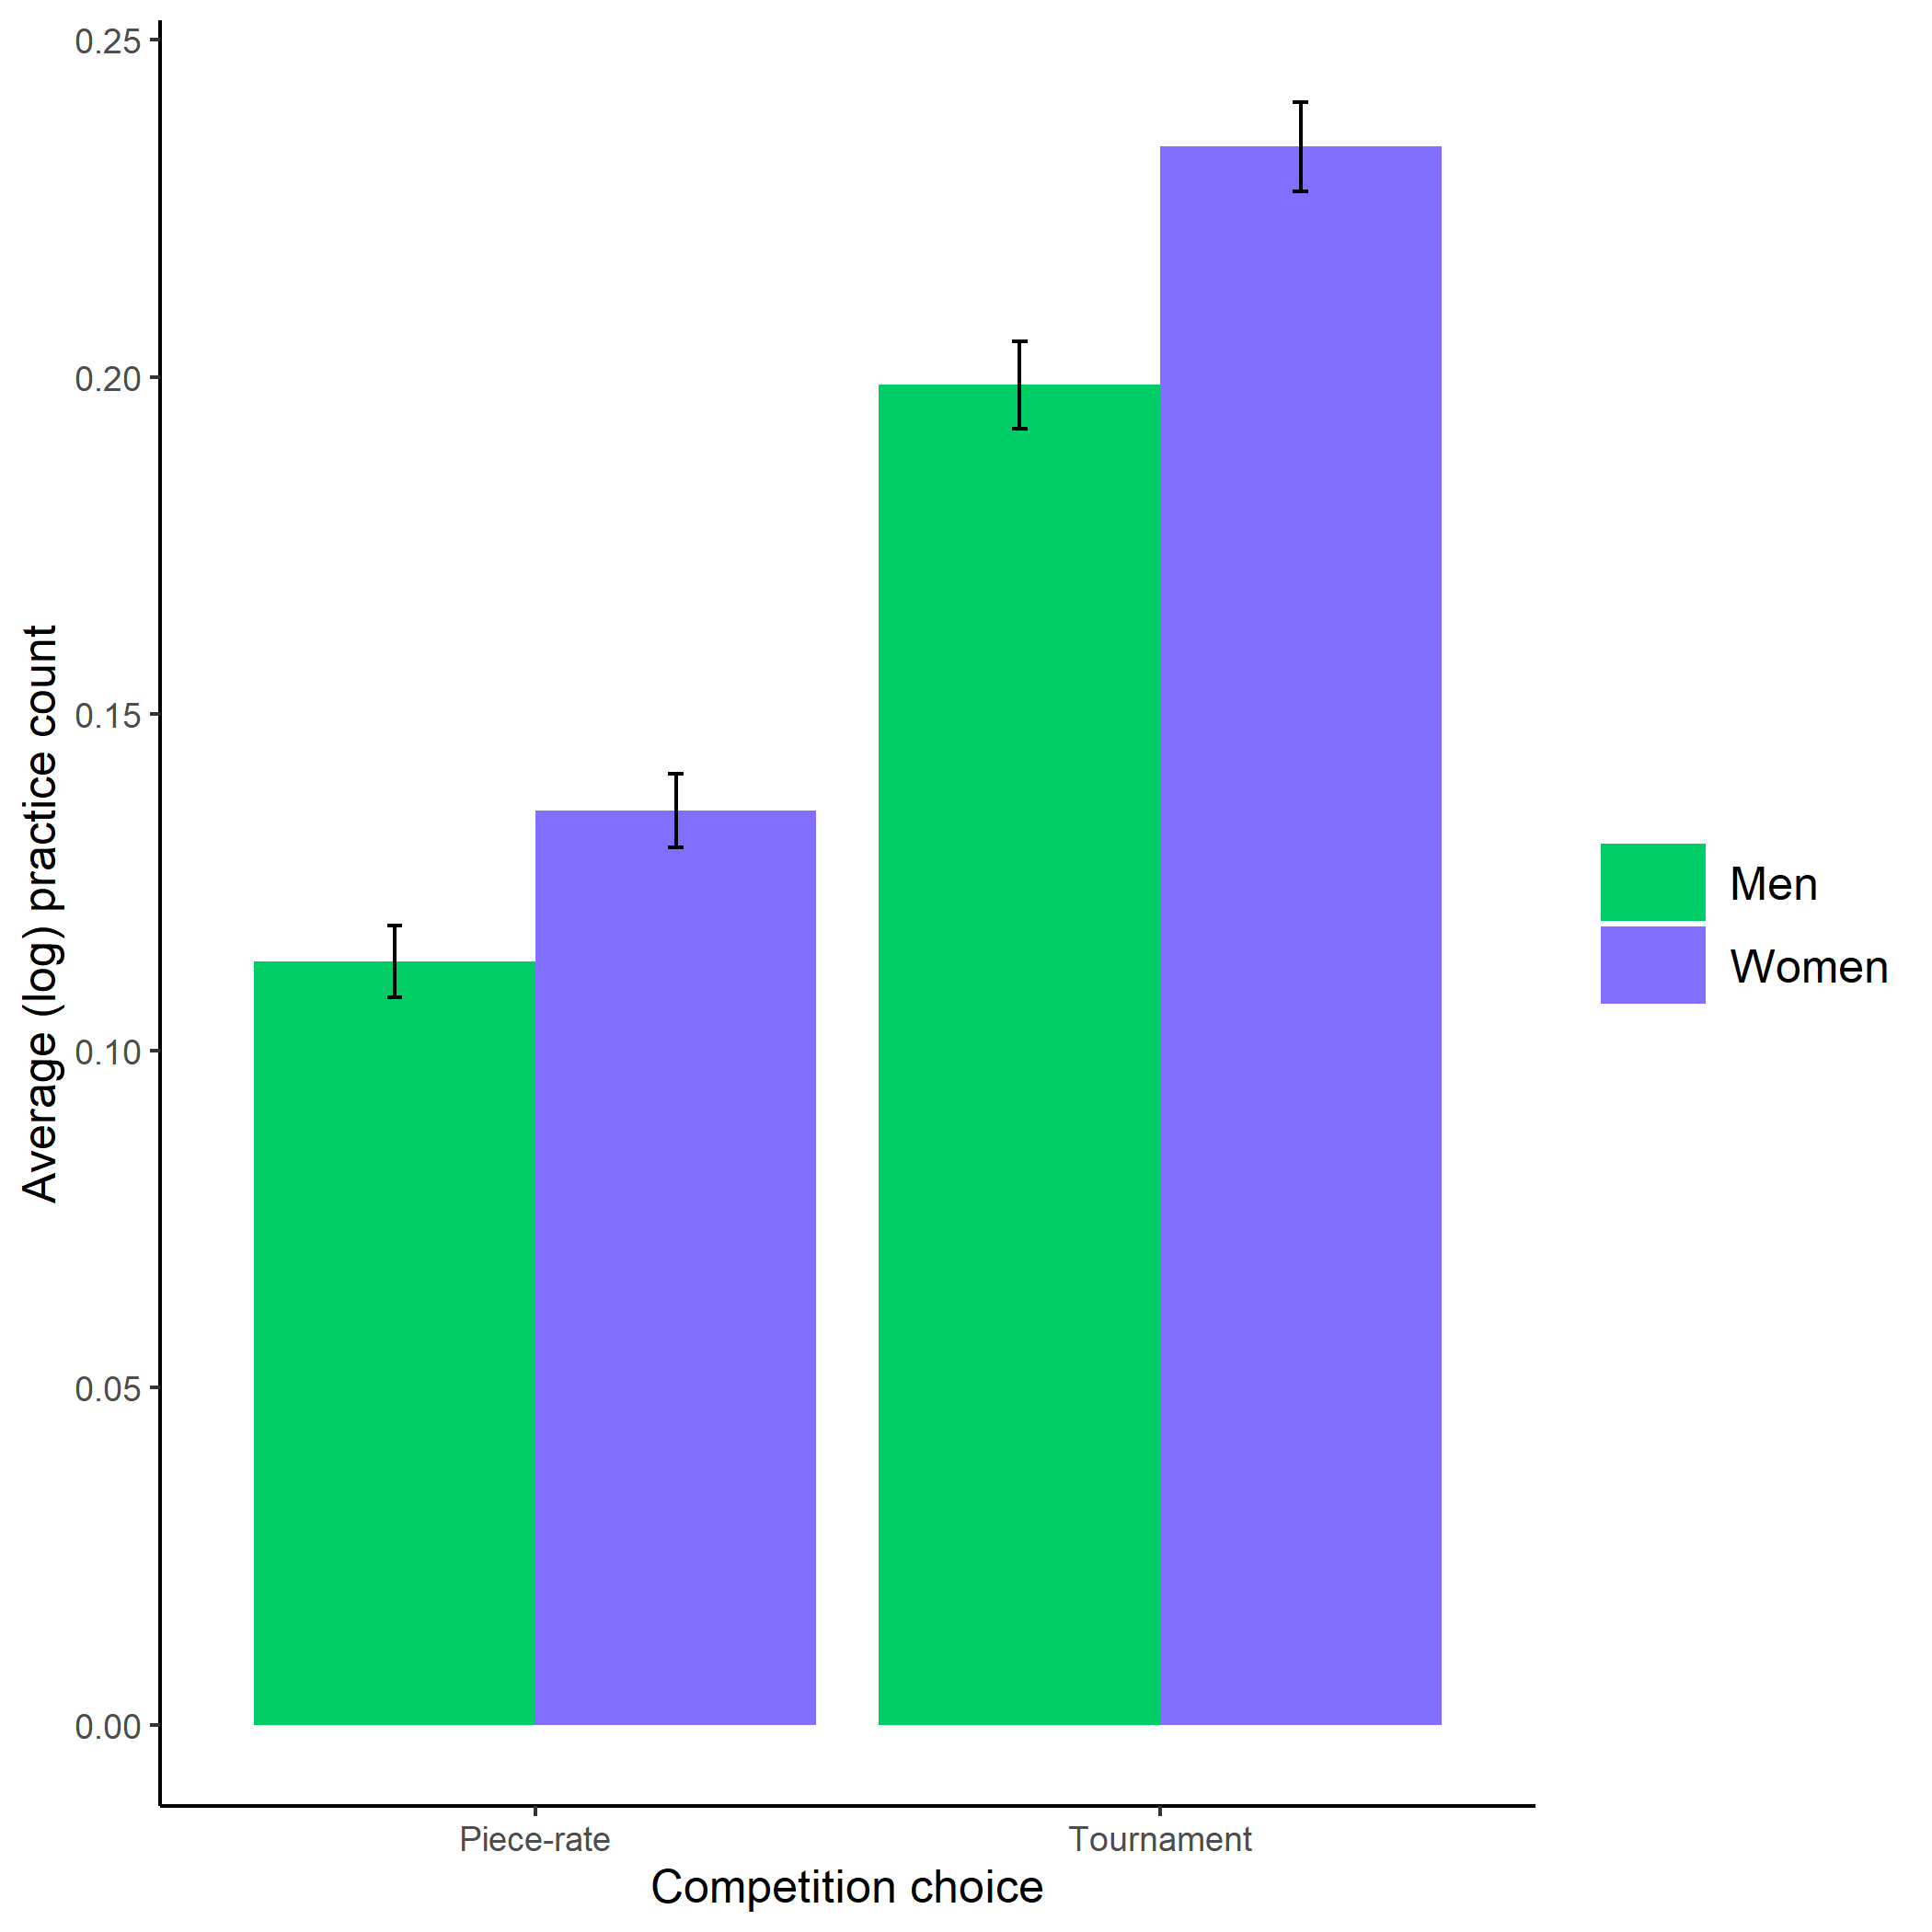
\includegraphics[width=29.17in]{C:/Users/keana/OneDrive - PennO365/Comp_transfer2018/Penn/practice_study/gender-practice/study2/figs/fig04_total-rev-count-by-gender-comp-choice} \caption{Gender differences in the number of extra preparation rounds chosen across participants' choice in a payment scheme. Here, we show that the gender gap in the choice to prepare is robust, even when half of the women are forced to prepare in the preparation condition. Error bars represent standard errors.}\label{fig:s204}
\end{figure}

\hypertarget{study-3-1}{%
\section{Study 3}\label{study-3-1}}

\begin{figure}
\includegraphics[width=29.17in]{C:/Users/keana/OneDrive - PennO365/Comp_transfer2018/Penn/practice_study/gender-practice/study4/figs/fig00_comp-choice-women-by-cond} \caption{Proportion of participants that identify as women who chose to compete by condition. We do not find evidence of the hypothesized effect of condition on the choice to compete. On the contrary, women in the control condition were significantly more likely to choose to compete than women in the preparation condition. Error bars represent standard errors.}\label{fig:s300}
\end{figure}

\begin{figure}
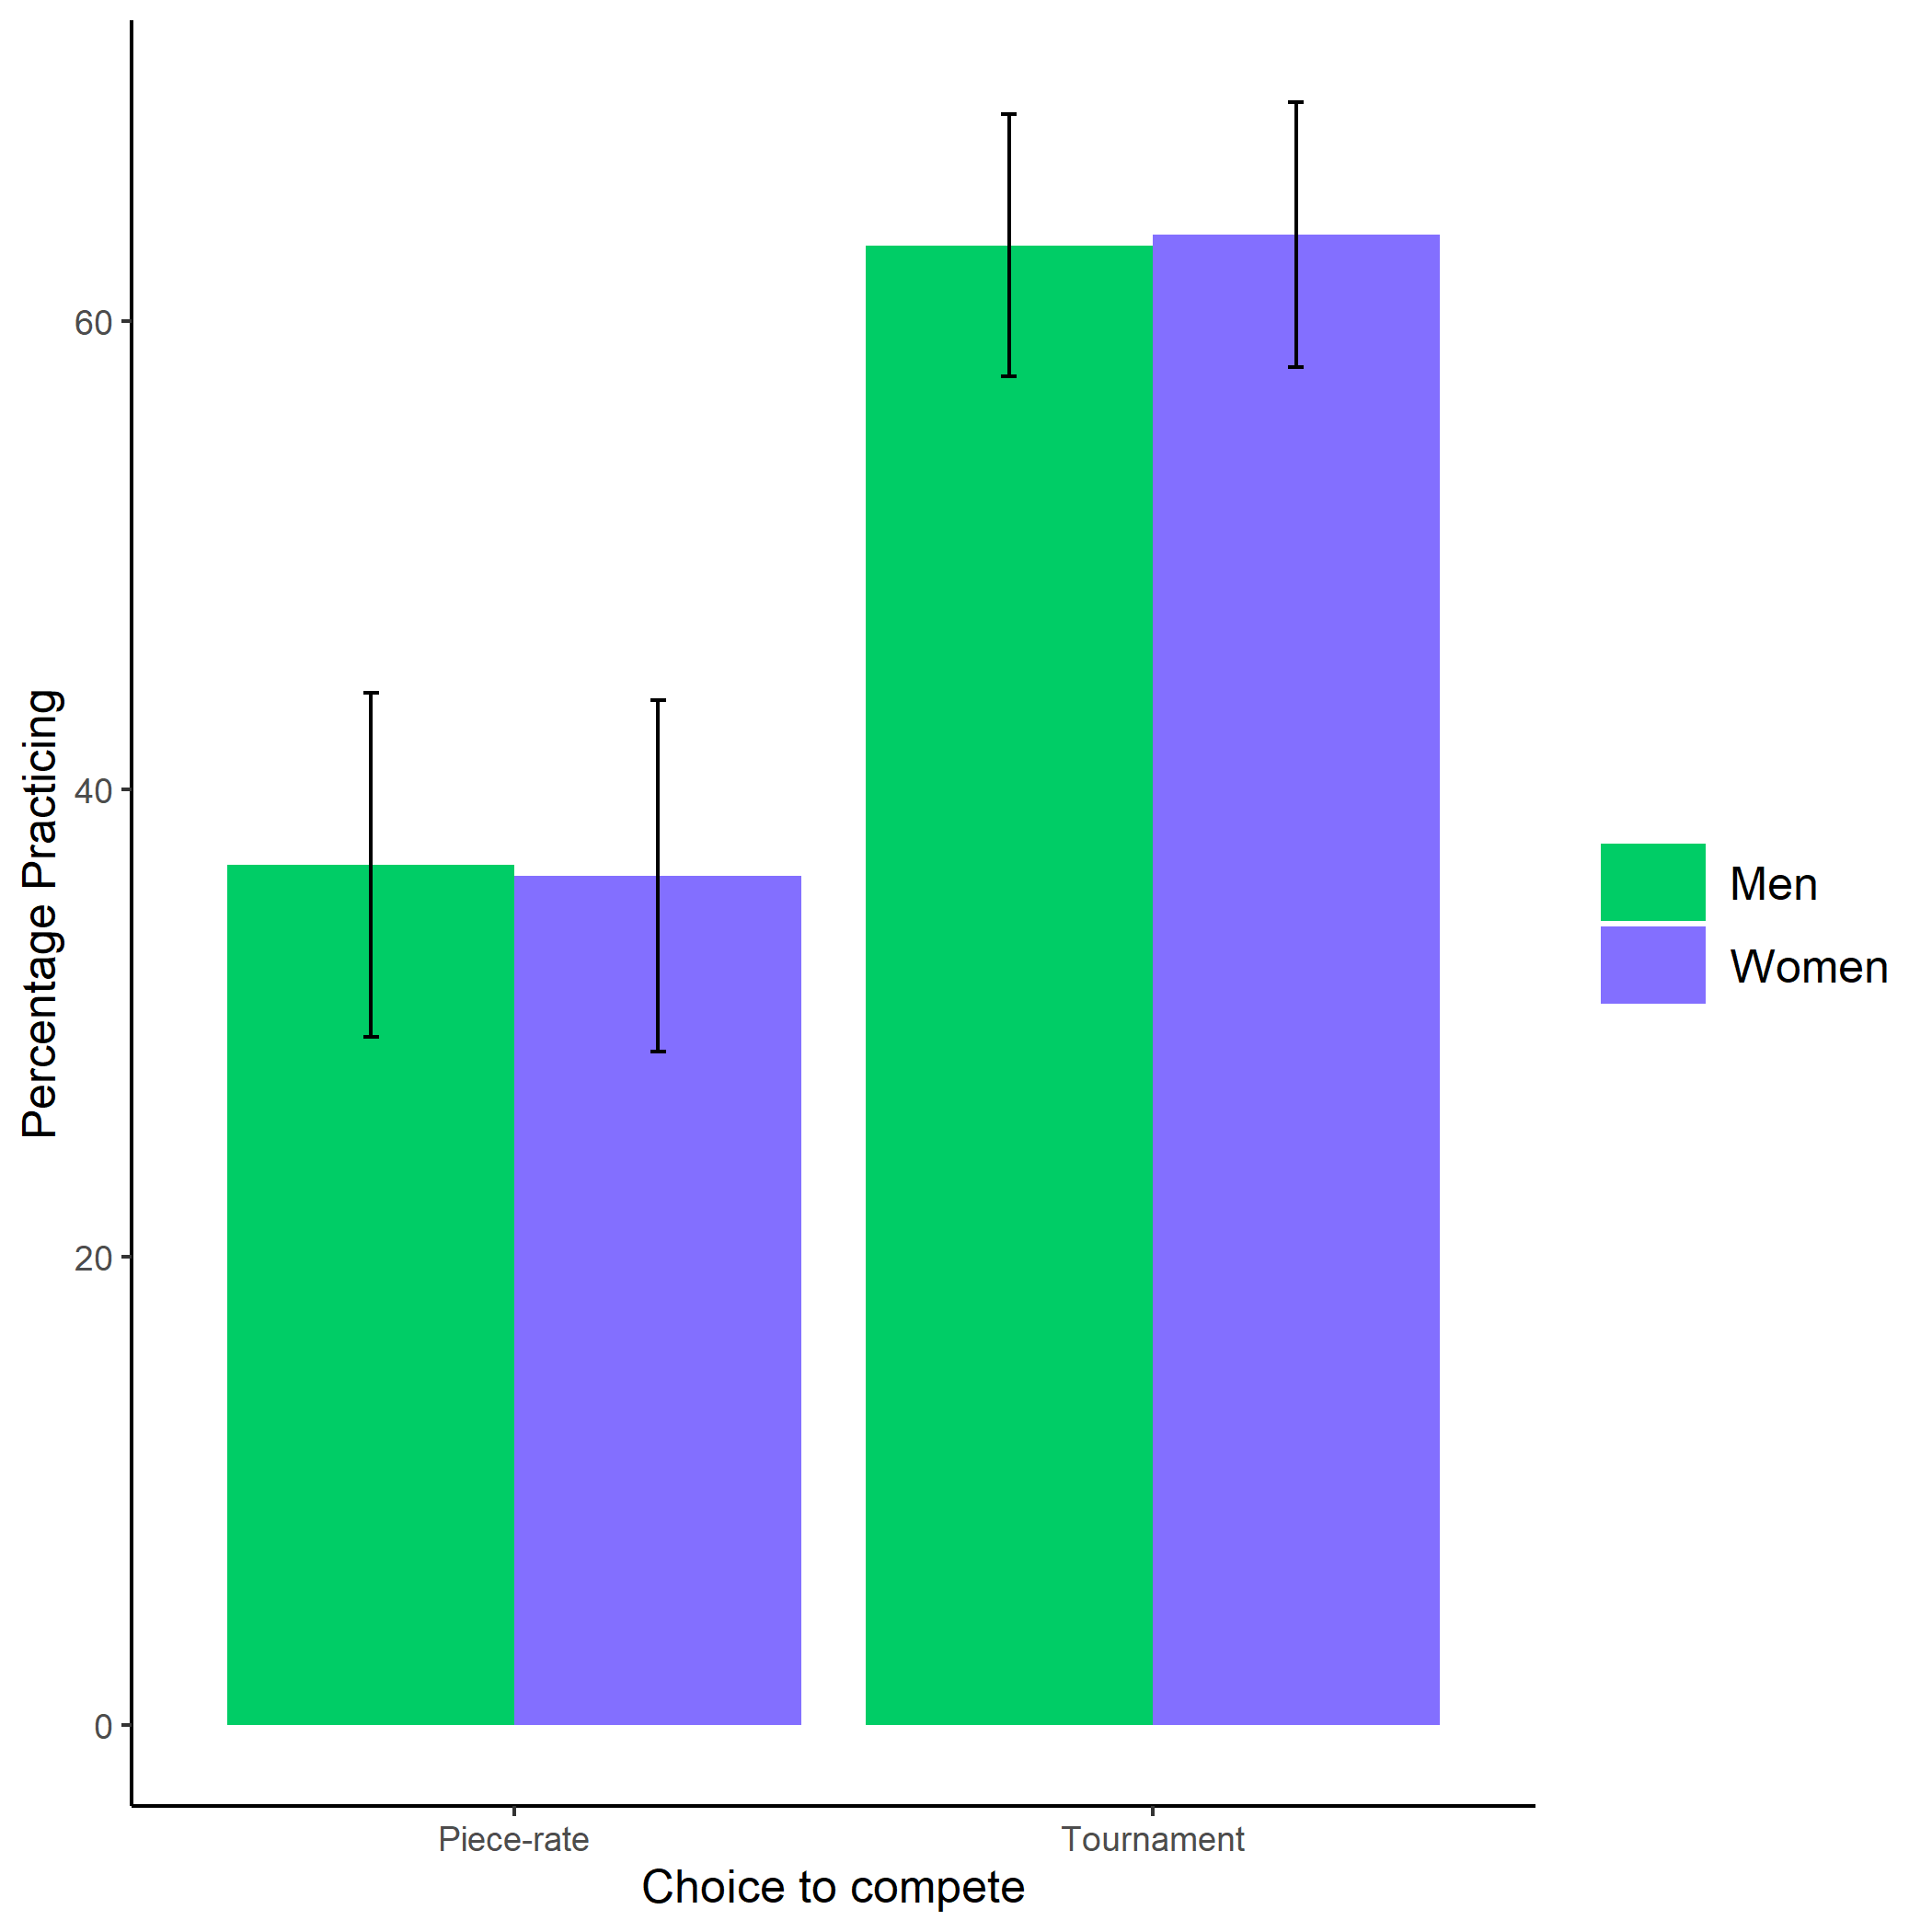
\includegraphics[width=29.17in]{C:/Users/keana/OneDrive - PennO365/Comp_transfer2018/Penn/practice_study/gender-practice/study4/figs/fig01_pract-choice-by-gender-and-cond-bar} \caption{Proportion of participants who chose to compete by condition and gender. We do not find evidence of the hypothesized interaction effect between condition and gender on the choice to compete. Error bars represent standard errors.}\label{fig:s301}
\end{figure}

\hypertarget{chapter-2-insert-title}{%
\chapter{Chapter 2: INSERT TITLE}\label{chapter-2-insert-title}}

\hypertarget{introduction-2}{%
\section{Introduction}\label{introduction-2}}

Possibly cut:

As the research on gender differences in performance during competition suggests \autocite{Gneezy2003,Gneezy2004,Gunther2010,Gill2014,Buser2019,Samak2013,Miller2019a}, it is important to consider potential downstream consequences of women's entry into competitions - before, during, and after a competition.

Another potential dimension of preparation that may manifest gender differences in preparation is the gender stereotypes about gender differences in preparation. talk about importance of stereotypes in driving behavior. and how people tend to feel good when they align with gender typical behavior (could draw from theory paper here). The most consistent finding in Chapter 1 of this dissertation is the beliefs about gender differences in preparation, both in terms of the multiplication task used across the studies and in general for most tasks.

\hypertarget{rising-use-of-performance-pay-especially-competitive-pay-over-time---and-how-it-may-contribute-to-the-gender-wage-gapother-gender-diff-in-labor-market-outcomes}{%
\section{Rising use of performance pay, especially competitive pay over time - and how it may contribute to the gender wage gap/other gender diff in labor market outcomes}\label{rising-use-of-performance-pay-especially-competitive-pay-over-time---and-how-it-may-contribute-to-the-gender-wage-gapother-gender-diff-in-labor-market-outcomes}}

Compensation packages based on performance pay, such as bonuses, commissions, and piece-rate payments, have risen in popularity relative to hourly/salaried pay, especially among workers in the highest tiers of occupations \autocite{Hall1998,Murphy1999,Cunat2005,Lemiuex2009}. There is evidence that the increasing use of performance pay lends itself to wage inequality. \textcite{Lemiuex2009} showed that an increased dependence on performance pay during the late 1970's and early 1990's accounted for 21\% of the observed growth in variance of male wages. Bonuses and commissions, arguably the most competitive compensation schemes, may be especially important in driving the large disparity between the highest and lowest percentile earners within organizations \autocite{Bell2010,Bell2014,Benabou2016}. Importantly, performance pay may contribute to the gender wage gap too. Using data from the National Longitudinal Surveys of Youth, \textcite{McGee2015} show that women are less likely to be employed in occupations that receive bonuses, and simultaneously are more likely to receive piece-rate pay -- the least competitive of all forms of performance pay, where workers are paid based on their absolute output.

\hypertarget{summary-of-literature-on-gender-differences-in-competitiveness}{%
\section{Summary of literature on gender differences in competitiveness}\label{summary-of-literature-on-gender-differences-in-competitiveness}}

Since competition is relevant to labor market outcomes, researchers began to focus on how a person's gender affects their competitiveness, both in terms of willingness to enter competitions and response when required to enter a competition. To date, most of the research on gender differences in competitiveness has focused on either i) explaining the sources of the gender difference \autocite[e.g.,][]{Veldhuizen2017} or ii) designing interventions to encourage women to compete more \autocite{Balafoutas2012,Sutter2016,Cassar2016,Brandts2015,Niederle2013,Brandts2015,Healy2011,Alan2018}. Less consideration has been paid to how competitions differentially, and negatively, impact women.

The introduction of Chapter 1 provides an overview of the literature on gender differences in willingness to compete, so we will only review the literature on gender differences in response to entering competitive environments here. There are three major time points at which competition may affect men and women differently: before, during, and after competition. The majority of previous studies in this space have examined gender differences in response to competition during and after performance, which we will briefly review here.

\hypertarget{gender-differences-in-response-to-competitive-environments}{%
\section{Gender differences in response to competitive environments}\label{gender-differences-in-response-to-competitive-environments}}

\hypertarget{during-competition}{%
\subsection{During competition}\label{during-competition}}

\hypertarget{gender-differences-in-performance-during-competition}{%
\subsubsection{Gender differences in performance during competition}\label{gender-differences-in-performance-during-competition}}

Although competitions are generally motivating and designed to improve performance through increased effort \autocite{Connelly2014a,Murayama2012,Miller2019a}, previous research suggests that men perform better under competitive payment schemes relative to non-competitive payment schemes, while women's performance does not respond to competitions \autocite{Gneezy2003,Gneezy2004,Gunther2010,Samak2013}. \textcite{Gneezy2003} show that there is no gender difference in performance when participants are solving mazes following a piece-rate payment scheme, but a significant gender difference in performance arises under a tournament payment scheme, with males performing better. \textcite{Gunther2010} replicate the effect of competition on gender differences in performance for a male-typed task, but find no gender differences in performance during competition for female-typed or gender-neutral tasks.

\hypertarget{after-competition}{%
\subsection{After competition}\label{after-competition}}

\hypertarget{gender-differences-in-response-to-losing}{%
\subsubsection{Gender differences in response to losing}\label{gender-differences-in-response-to-losing}}

Relatedly, during repeated competition, women tend to perform worse in subsequent performance rounds after losing, even if the monetary prize they lost was relatively meager, while men only perform worse in subsequent rounds if they lost the chance to win a large monetary prize \autocite{Gill2014}. Other research suggests women stop competing altogether after losing if given the choice. \textcite{Buser2019}, who examine the effects of losing while competing in the Dutch Math Olympiad on the choice to compete in subsequent years, show that men are just as likely to compete even if they lost the previous year, while women are less likely to compete again if they lost before. Overall, this body of literature suggests that competitions may differentially impact women and men, both during and after the competition.

\hypertarget{before-competition}{%
\subsection{Before competition}\label{before-competition}}

As mentioned previously, little research has examined how competitions may affect gender differences in behavior during arguably the most critical period: before an individual enters a competition, where they have the most control of their subsequent performance in the competition. For that reason, we provide a broad overview of how people generally respond before competitions based on the feelings they tend to elicit, which leads us to our hypotheses about gender differences in behavior before competition entry.

\hypertarget{what-feelings-does-competition-cause-before-entry-what-does-previous-research-suggest-about-how-people-feelrespond-before-they-compete-that-may-cause-them-to-use-coping-mechanisms-may-not-be-a-necessary-section}{%
\subsubsection{What feelings does competition cause before entry? What does previous research suggest about how people feel/respond before they compete that may cause them to use coping mechanisms? (May not be a necessary section)}\label{what-feelings-does-competition-cause-before-entry-what-does-previous-research-suggest-about-how-people-feelrespond-before-they-compete-that-may-cause-them-to-use-coping-mechanisms-may-not-be-a-necessary-section}}

\hypertarget{coping-strategies-people-may-use-before-entering-a-competition-may-not-be-necessary-to-include-others-just-prep}{%
\subsubsection{Coping strategies people may use before entering a competition (may not be necessary to include others, just prep)}\label{coping-strategies-people-may-use-before-entering-a-competition-may-not-be-necessary-to-include-others-just-prep}}

There are a number of strategies people may use to cope with entering a competition and how it may help with aforementioned feelings before competing

\begin{itemize}
\tightlist
\item
  INSERT list of possible strategies outside of preparation
\end{itemize}

Finally, preparing for a competition, through either practicing or studying, is another potential response to entering a competition. Describe how it may help (draw from intro of previous chapter)

explain why we are focusing on preparation instead of other possible coping mechanisms

\hypertarget{gender-differences-in-preparation-and-beliefs-about-relative-preparation---aka-current-study-hypotheses-what-we-think-is-driving-it.}{%
\subsubsection{Gender differences in preparation and beliefs about relative preparation - aka current study hypotheses \& what we think is driving it.}\label{gender-differences-in-preparation-and-beliefs-about-relative-preparation---aka-current-study-hypotheses-what-we-think-is-driving-it.}}

Given previous research suggesting that women and men may respond differently during and after competitions, we expect that they will also employ different behaviors and have different perceptions of themselves and others in advance of a competition.
Here, we focus on how women and men differentially respond to competition through preparation, expanding upon the studies in Chapter 1 by directly manipulating whether participants are competing.

My previous research provides evidence of this gender difference in preparation. but need to explain why it may not be reliable (repeating from Ch 1)

HYPOTHESIS I: Women will choose to practice problems at a higher rate than men, especially when assigned to the competitive tournament payment scheme (i.e., we anticipate a main effect of gender on practice, and an interaction between gender and condition, such that women will practice more than men in both conditions, but the difference-in-differences between practicing rates across genders will be greater in the competition condition).

We expect that this gender difference is driven by the aforementioned gender differences in risk attitudes and confidence

\begin{itemize}
\tightlist
\item
  could also be driven by both gender stereotypes and task stereotypes
\end{itemize}

\hypertarget{confidence-and-risk-attitudes-as-possible-explanations-for-gender-difference-in-preparation-especially-when-required-to-compete}{%
\paragraph{Confidence and risk attitudes as possible explanations for gender difference in preparation, especially when required to compete}\label{confidence-and-risk-attitudes-as-possible-explanations-for-gender-difference-in-preparation-especially-when-required-to-compete}}

Since competitions, by definition, compare the performance among two or more individuals, they naturally lead to self-evaluation and comparative judgments of self with others - processes that are intimately linked to confidence. To the extent that confidence influences how much individuals think they need to prepare in order to win, we may expect to see women preparing more than men, particularly in competitive contexts, which naturally invoke self-other assessments. Thus, less confident individuals may prepare more. Moreover, they may prepare more in order to reduce the negative feelings caused by low confidence independent of any ambitions to win, since mastery is an important driver of confidence \autocite{Gist1992,Usher2008}. There is no theoretical or empirical reason to suspect that women would be less concerned with mastery than men. In fact, research suggests that women are just as likely as men to compete when competing against their own past performance, suggesting, at minimum, an equal desire for self-improvement \autocite{Apicella2017a}. Similarly, given the inherent risk of competitive payment schemes relative to non-competitive payment schemes, it is possible that the aforementioned gender differences in risk attitudes may also lead women to be more likely to cope by preparing before performing in a competition relative to men.

Perceptions of relative preparation

\begin{itemize}
\tightlist
\item
  Even if risk and confidence do not affect actual preparation behavior,
\end{itemize}

Women may have a tendency to feel as though they are not preparing enough before performance, regardless of how much they actually practice (aka exploratory analysis looking at how much women prepare) - arguably driven by same possible explanations for gender differences in risk and confidence. - although we do not find strong evidence that confidence or risk are strongly related to practicing (2X check)(however, it was not a main hypothesis so the effect would need to be explored further in future studies)

HYPOTHESIS II: Women will be more likely to assume they practice less than others compared to men (that is, the effect of gender on perceived practice deviation will be negative), especially when assigned to the competitive tournament payment scheme (such that women in general will think that they practice less than other participants than men, but this difference will be exacerbated in the competition condition).

Possible explanations:
- could be driven by gender stereotypes (which we find evidence for in previous Chapter - 2X check)
- driven by risk \& confidence

Thus, we expect to see both gender differences in actual preparation behavior, along with gender differences in perceptions of relative preparation.

INTEGRATE:

Overall, women may engage in more coping strategies, such as preparation, before entering competitions because they tend to be more risk-averse \autocite{Croson2009,Dohmen2011b,Eckel2008,Bertrand2010a}, less confident \autocite{Bertrand2010,Lundeberg1994,Mobius2011,Barber2001,Croson2009} and prefer to opt out of competitions \autocite{Niederle2011}. In fact, in Chapter 1 of this dissertation, we find evidence of a sizable gender difference in effort, where women were more likely than men to choose to prepare before completing a multiplication task. To be clear, there was no interaction between gender and choice to compete on the choice to prepare in any of the previous studies. That is, women prepared more than men regardless of which payment scheme they had chosen. However, it is not possible to draw conclusions from this because i) we did not manipulate the payment scheme, so there could have been selection effects on one's choice to prepare across payment schemes, such that those who were more likely to choose to compete may have been less likely to prepare, and ii) there was little power to detect any possible interaction effects. For instance, in the first study, only 11\% {[}DOUBLE CHECK{]} of women chose to compete, and in the second, INSERT\% of women made this decision. Through the proposed experiments, we intend to address these limitations by directly manipulating participants' payment scheme and recruiting a large sample to provide power to detect small effects.

Chapter 2 of this dissertation builds on prior research by examining how competitions affect gender differences in the amount of time spent preparing for competitions. We hypothesize that women will spend more time preparing than men, especially before competitions, in part because they are, on average, less risk-seeking \autocite{Croson2009,Dohmen2011b,Eckel2008,Bertrand2010a} and confident \autocite{Bertrand2010,Lundeberg1994,Mobius2011,Barber2001,Croson2009} than men. Indeed, both confidence and risk attitude have been implicated in driving the gender gap in willingness to compete \autocite{Niederle2011,Veldhuizen2017} (see Chapter 1 introduction for a more detailed review of the previous literature on gender differences in risk and confidence).

In the study included in this chapter, we tested whether competition exacerbates previously established gender differences in preparation by manipulating participants' assigned payment scheme (i.e., competitive or non-competitive). We also explored whether gender predicts participants' perceptions of their relative amount of preparation, given our hypothesis based on Study 3 of Chapter 1 that women may be especially susceptible to feelings of underpreparation relative to others when they have unlimited time to prepare. The research design, hypotheses, measures and analyses for this chapter were pre-registered on \href{INSERT\%20LINK}{OSF} and all analyses were conducted in R statistical software (version 4.0.4).

\hypertarget{discussion-4}{%
\section{Discussion}\label{discussion-4}}

idea from Coren to integrate:

One thing we should consider, based on Emily's question in the last email, is that perhaps women, compared to men, ``take time'' before the competition. That is, they might not be studying, but rather are delaying the competition (i.e., taking a breather, prepping emotionally, etc) by looking at their phones, taking a bathroom break etc. In other words, if men are more eager to compete then any differences in time spent in practicing could reflect a gender difference in ``eagerness'' to get to the competition. I don't want to change anything, of course, but I think we should just be aware of it and perhaps address it in the write-up. Hopefully, we will see a decent relationship between time and \#of problems practiced. :)

note to self: pulled from nsf app 01\_project-description.Rmd

\hypertarget{broader-impacts}{%
\chapter{Broader impacts}\label{broader-impacts}}

Much of the research on gender differences in competitiveness has focused on designing interventions that increase women's willingness to compete. Less work has paid attention to the downstream consequences of said interventions. If we find that women spend more time preparing on average than men, and possibly overprepare, this would challenge prevailing views that gender differences in labor market outcomes could be reduced or eliminated by simple interventions. Indeed, there are opportunity costs to (over)preparing, including both economic and social costs, such as lost time with family and friends and missed advancement opportunities.

Relatedly, if women \emph{expect} that they will prepare more in competitive environments, this may, in turn, impact whether they even enter competitive environments. Thus, while our prior work suggests that merely giving women more time to prepare does not make them more willing to compete (Richards et al., in prep), anticipated effort could still influence labor market outcomes by affecting women's decisions to enter certain fields or compete for promotions, for instance. In our studies, we use relatively unimportant tasks that are unlikely to greatly impact one's earnings. Yet, our previous work shows a striking gender difference in preparation, suggesting that our study likely \emph{underestimates} gender differences in choices to prepare for tasks that are more important for one's career and economic prospects. In this way, our study is providing a conservative test of the gender differences in effort and preparation in the real world.

\hypertarget{future-directions}{%
\chapter{Future directions}\label{future-directions}}

There are a number of avenues for future research in this area. First, we would like to test the robustness of gender differences in preparation outside of online and laboratory settings. Do these findings translate to real-world settings? Exploring the gender difference in preparation cross-culturally would also shed light on the universality of the finding and help to identify cultural, ecological and social factors that exacerbate it. Given Dr.~Apicella's expertise on cross-cultural research, including work with hunter-gatherers \autocite{Apicella2014a,Apicella2012,Apicella2017,Apicella2015,Apicella2009,Apicella2015a,Apicella2018,Apicella2007,Apicella2014,Apicella2016,Apicella2018a,Apicella2007a}, exploring the generalizability of these findings across cultures is a real possibility.

A second important extension of the work would be to examine how anticipated preparation or workload influences women's decisions to enter competitive environments. While we did not find that giving women time to prepare makes them more likely to compete, it is still possible that women know that they will end up preparing more in competitive situations and thus, select out of them. As mentioned earlier, there are opportunity costs to preparing.

A third extension of the current work would be to examine whether women are overpreparing. Does preparation negatively impact women? Does it help women? To determine whether men or women are preparing more (or less) than needed, future research should test whether gender and time chosen to prepare interact to affect a participants' probability of winning a competition \autocite[see][]{Niederle2007}. Another follow-up study could manipulate whether there is a monetary cost for preparing to explore whether gender differences in the choice to prepare persist despite a clear cost, and whether this leads to gender differences in earnings within the study.

-- IMPORTANT: based on the results from these set of studies, we recommend future research explore the concept of changing the systmem, rather than changing women (see \url{https://www.nber.org/system/files/working_papers/w26345/w26345.pdf} conclusion section for more cites on changing the system approaches)

While we build off an extensive and laudable literature on gender differences in competitiveness, we have unearthed a gender difference in preparation. As this is a new area of research, there are many promising and exciting avenues for future exploration, all of which have the potential to inform policies that mitigate gender disparities in the labor market.

\hypertarget{figures-1}{%
\section{Figures}\label{figures-1}}

\hypertarget{discussion-5}{%
\chapter*{Discussion}\label{discussion-5}}
\addcontentsline{toc}{chapter}{Discussion}

\adjustmtc
\markboth{Introduction}{}

Welcome to \texttt{oxforddown} \autocite{lyngsOxforddown2019}, a thesis template for R Markdown that I created when writing \href{https://ulyngs.github.io/phd-thesis/}{my own PhD thesis} at the University of Oxford.
This template allows you to write in R Markdown, while formatting the PDF output with the beautiful and time-tested \href{https://github.com/mcmanigle/OxThesis}{OxThesis LaTeX template}.
The sample content is partly adapted from \href{https://github.com/ismayc/thesisdown}{\texttt{thesisdown}}

\startappendices

\hypertarget{chapter-1}{%
\section{Chapter 1}\label{chapter-1}}

\hypertarget{study-3-comparing-results-with-vs.-without-fradulent-responses}{%
\subsection{Study 3: Comparing results with vs.~without fradulent responses}\label{study-3-comparing-results-with-vs.-without-fradulent-responses}}

\begin{itemize}
\tightlist
\item
  In Keana's last study, she used this software to detect fraudulent responses (n=67). For her dissertation, she planned to run the analyses using the full data set and then again with the fraudulent responses removed. I suggested that for this prior study, she remove the ``fraudulent responses'' from her main analyses, noting this departure from her preregistration. I also suggested that she include the analyses for the full sample in her appendix, but that she should note in her dissertation that the results remain largely unchanged (I assume they do). Does this approach sound ok to everyone?
\end{itemize}

\hypertarget{chapter-2}{%
\section{Chapter 2}\label{chapter-2}}

\hypertarget{comparing-results-with-vs.-without-fradulent-responses}{%
\subsection{Comparing results with vs.~without fradulent responses}\label{comparing-results-with-vs.-without-fradulent-responses}}

\begin{itemize}
\tightlist
\item
  See Chapter 1 appendix section
\end{itemize}


%%%%% REFERENCES
\setlength{\baselineskip}{0pt} % JEM: Single-space References

{\renewcommand*\MakeUppercase[1]{#1}%
\printbibliography[heading=bibintoc,title={\bibtitle}]}


\end{document}
